\documentclass[12pt twoside]{report}
% \documentclass{book}

\def\blankpage{%
      \clearpage%
      \thispagestyle{empty}%
      \addtocounter{page}{-1}%
      \null%
      \clearpage} 


% includes
\usepackage{geometry}           % page size
\usepackage[utf8]{inputenc}     % encoding
\usepackage{palatino}           % font
\usepackage[english]{babel}     % language
\usepackage{graphicx}           % images
\usepackage{indentfirst}        % indentation
\usepackage[nottoc]{tocbibind}  % table of contents style
\usepackage[unicode]{hyperref}  % references from the table of contents
\usepackage{wrapfig}            % for the small images that have text around
\usepackage[rightcaption]{sidecap}
\usepackage{amsmath}            % for math cases in functions
\usepackage{xcolor}
\usepackage{fancyhdr}
% Set the page style to "fancy"...
\pagestyle{fancy}


% %... then configure it.
% \fancyhead{} % clear all header fields
% \fancyhead[RO,LE]{\textbf{The performance of new graduates}}
% \fancyfoot{} % clear all footer fields
% \fancyfoot[LE,RO]{\thepage}
% \fancyfoot[LO,CE]{From: K. Grant}
% \fancyfoot[CO,RE]{To: Dean A. Smith}


\usepackage{tikz}
\usepackage{pgfplots}



% includes options
\geometry{  a4paper,            % scientific thesis standard
            left=3cm,
            right=2cm,
            top=2cm,
            bottom=2cm,
 }
\graphicspath{{src/img/}}        % path where the images are located
\setlength{\parindent}{1cm}     % paragraph indentation

% other options
\linespread{1.5}                % space between lines
\renewcommand*\contentsname{Table of contents}    % table of contents name




% FOR PROGRAMMING SNIPPETS


\usepackage{listings} % For code listings
\usepackage{xcolor}   % For coloring code

% Define colors for code highlighting
\definecolor{codegreen}{rgb}{0,0.6,0}
\definecolor{codegray}{rgb}{0.5,0.5,0.5}
\definecolor{codepurple}{rgb}{0.58,0,0.82}
\definecolor{backcolour}{rgb}{0.95,0.95,0.92}

% Define C++ code style
\lstset{
    language=C++,
    backgroundcolor=\color{backcolour},   
    commentstyle=\color{codegreen},
    keywordstyle=\color{blue},
    numberstyle=\tiny\color{codegray},
    stringstyle=\color{codepurple},
    basicstyle=\footnotesize\ttfamily,
    breakatwhitespace=false,
    breaklines=true,
    captionpos=b,
    keepspaces=true,
    numbers=left,
    numbersep=5pt,
    showspaces=false,
    showstringspaces=false,
    showtabs=false,
    tabsize=2,
    frame=single
}





% the document content
\begin{document}
    % macros (global)
    \newcommand{\university}    {"Alexandru-Ioan Cuza" University}
\newcommand{\universityg}   {Universității "Alexandru-Ioan Cuza" din Iași} % genitive
\newcommand{\faculty}       {Computer Science}
\newcommand{\facultyg}      {Facultății de informatică} % genitive
\newcommand{\speciality}    {Computer Science}
\newcommand{\promotion}     {2024}                                  %<---------

\newcommand{\thesistype}    {Thesis Paper}
\newcommand{\thesistitle}   {Machine Learning Compatible Game Engine}    %<---------

\newcommand{\authorlast}    {Bobu}                               %<---------
\newcommand{\authorfirst}   {Dragoş-Andrei}
\newcommand{\authornamefl}  {\authorfirst \space \authorlast} % first name first
\newcommand{\authornamelf}  {\authorlast \space \authorfirst} % last name first
\newcommand{\authorbirth}   {06 iulie 2001}                      %<---------
\newcommand{\authoraddress} {România, jud. Iași, mun. Iași, Valea lupului, str. Nufarului, nr 18} %<---------
\newcommand{\authorcnp}     {5010607374511}                         %<---------

\newcommand{\session}       {July, 2024}                       %<---------
\newcommand{\coordinator}   {Dr. Cosmin Varlan, Lecturer}               %<---------

\newcommand{\dottedline}    {............................}

    
    % front-matter
    \pagenumbering{gobble}








    \blankpage
    % define the cover page
\begin{titlepage}
    \begin{center}
        % the university and faculty
        \large
        \MakeUppercase{\university}
        
        \LARGE
        \textbf{\MakeUppercase{\faculty}}
        
        % the faculty logo
        \vspace{1cm}
        
\includegraphics[width=0.3\textwidth]{logoFii.png}
        
        % thesis title
        \vspace{1cm}
        \Large
        \MakeUppercase{\thesistype}
        
        \vspace{0.5cm}
        \LARGE
        \textbf{\thesistitle}
        
        % author
        \vspace{2cm}
        \Large
        author
        
        \vspace{0.5cm}
        \LARGE
        \textbf{\authornamefl}
        
        % session
        \vfill
        \Large
        \textbf{session:} \session
        
        % scientific coordinator
        \vspace{2cm}
        \Large
        scientific coordinator
        
        \vspace{0.5cm}
        \LARGE
        \textbf{\coordinator}
    \end{center}
\end{titlepage}
    \blankpage
    % define the title page
\begin{titlepage}
    \begin{center}
        % the university and faculty
        \large
        \MakeUppercase{\university}
        
        \LARGE
        \textbf{\MakeUppercase{\faculty}}
        
        % thesis title
        \vspace{8cm}
        \huge
        \textbf{\thesistitle}
        
        % author
        \vspace{2cm}
        \LARGE
        \textbf{\authornamefl}
        
        % session
        \vfill
        \Large
        \textbf{Session} \session
        
        % scientific coordinator
        \vspace{4cm}
        \Large
        Scientific Coordinator
        
        \vspace{0.5cm}
        \LARGE
        \textbf{\coordinator}
    \end{center}
\end{titlepage}

    \blankpage

    \setcounter{page}{1}
    \pagenumbering{arabic}
    






    % \blankpage



    % \part*{Abstract}
    

Computer Software is just a bunch of tools orchestrated in just the right manner.


Similarly to this, a game engine is just a software framework of computer graphics components.


The Game Editor is what allows users to custom build new tools that work seemingly with the already existing SOLID engines.



    % \fancyhead{} % clear all header fields




    % table of contents
    \tableofcontents






    \part{Introduction}
      \section*{Motivation}
          




% This project aims to develop into a robust service featuring numerous endpoints, enabling users to leverage its unique set of components to create graphical experiences.

% This edition's update journal will review the implementation status of the initial building blocks in the toolkit.


% This project wished to evolve into a solid service with many endpoints that users can benefit from it's unique collection of components in order to build graphical experiences.



% This edition's update journal will iterate over the implementation status of the first building blocks in the toolkit. 

The immersiveness of games could be significantly enhanced by integrating machine learning (ML) with the existing dialogue tree frameworks. Such integration has the potential to create more dynamic and responsive NPC interactions.













      \section*{Introduction}
          









\fancyhead{} % clear all footer fields

\fancyhead[L]{INTRODUCTION}
\fancyhead[C]{}
\fancyhead[R]{MOTIVATION}
Non-Player Characters (NPCs) serve as guides for players and act as extensions of the game designers within the game world. Consequently, it is crucial for NPCs to have fluid dialogue that maintains the illusion of choice without easily breaking it.

Currently, dialogue trees are the predominant solution for managing NPC interactions. While effective, dialogue trees can still feel somewhat rigid and may disrupt the immersion when players are limited to selecting from a set of predefined responses.





















          




\begin{wrapfigure}{r}{0.25\textwidth} %this figure will be at the right
    \centering
    % \includegraphics[width=0.35\textwidth]{game_engine}
\end{wrapfigure}

This implementation required extensive study across multiple fields of computer science, including:

\begin{itemize}
\item Computer Graphics
\item Game Development
\item Machine Learning
\end{itemize}


Additionally, the following courses have provided essential tools and skills that have significantly contributed to the success of this project:

% Additionally, courses such as the following have equipped me with the skills to be an agile and resourceful developer:

\begin{itemize}
\item Object-Oriented Programming, Data Structures, and Software Engineering
\item Python Programming, Programming Language Principles, and Logics
\end{itemize}










% This implementation required extensive study of multiple computer science fields. 
% Out of which i will name a few: 

% \begin{itemize}
%   \item Computer Graphics
%   \item Game     Development
%   \item Machine  Learning
% \end{itemize}


% % \includegraphics[width=0.8\textwidth]{courses.png}



% Beside those, courses such as the following had made me an agile handyman that has his toolbox in order:
% \begin{itemize}
%   \item oop, data structures and Software Engineering
%   \item python programming, plp and Logics
% \end{itemize}

% % \includegraphics[width=0.8\textwidth]{courses2.png}



















          % \begin{center}
          % \includegraphics[width=0.9 \textwidth]{game_engine_overview.png}
          % \end{center}

          
  % \fancyfoot[C]{* = More information about game engines will follow in the \hyperlink{GameEngines}{Field Study} chapter}





\begin{center}
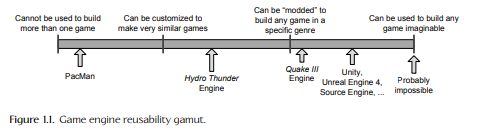
\includegraphics[width=0.9 \textwidth]{game_engine_process.png}
\end{center}



\begin{center}
  \underline{\textbf{Game Engines are essential not only for games but also for other diverse applications.}}

  \emph{Each Game Engine defines its functionality through its implemented components.}
\end{center}





%% TODO TODO IMAGES




% \begin{center}
% 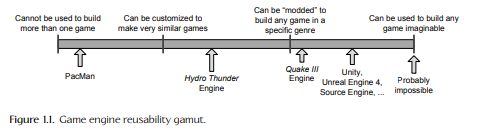
\includegraphics[width=0.9 \textwidth]{game_engine_process.png}
% \end{center}






% 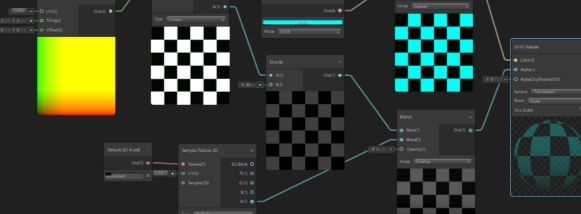
\includegraphics[width=10cm]{unity_shader}

% \begin{figure}[h]
% 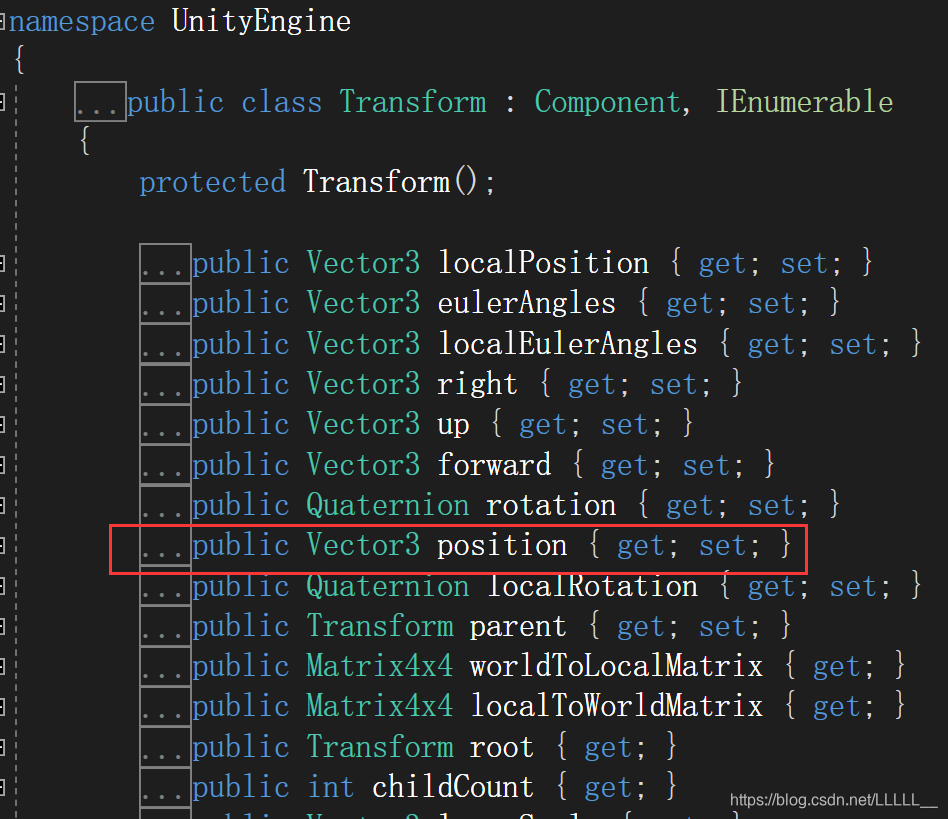
\includegraphics[height=5cm]{unity_transform}
% 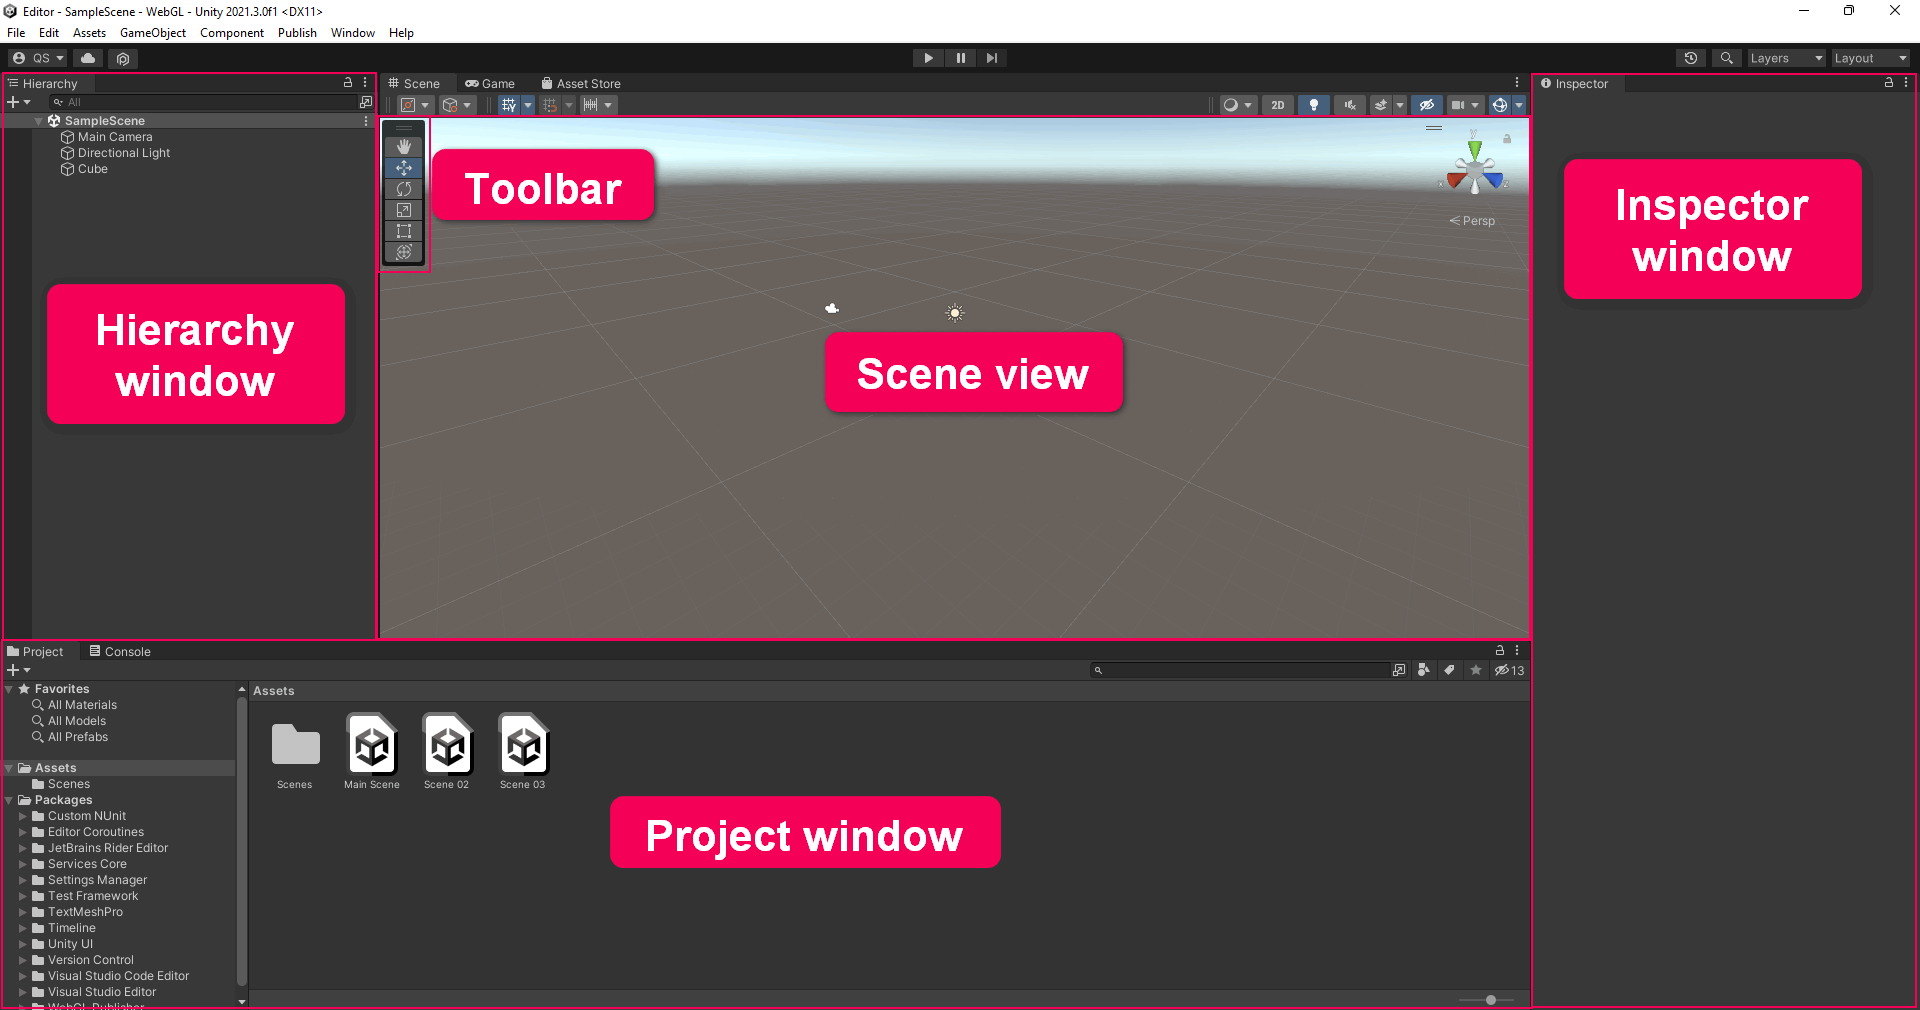
\includegraphics[height=5cm]{unity_editor}
% \end{figure}



          \pagebreak

          \fancyhead[L]{}
          \fancyhead[C]{Problem Statement}
          \fancyhead[R]{}
          








\section*{Problem Statement}

\textbf{Definition Setup:}

Let \( S \) denote a software entity. The function \( \text{isGameEngine}(S) \) outputs true if \( S \) qualifies as a game engine based on the following criteria:

\[
\text{isGameEngine}(S) \equiv \text{isFramework}(S) \land (\{ S.\text{components} \} \subseteq \text{GE::E})
\]

Where:
\begin{itemize}
    \item \( \text{isFramework}(S) \) indicates that \( S \) is classified as a software framework.
    \item \( \text{GE::E} \) represents the set of components common to various game engines, defined as:
    \[
    \text{GE::E} = \bigcup_{G_i \in \text{GameEngines}} \{ (G_i, C_j) \mid C_j \in \{ G_i.\text{components} \} \}
    \]
\end{itemize}

\textbf{Scenario:}

Assume a scenario where a company is developing a new game engine, \( GG \), which includes the following components: MathEngine (M), RendererEngine (R), GUI Editor (E), and File Manager (FM).

1. Define \( GG \) as:
\[
GG = \{ M, R, E, FM \}
\]

\textbf{Tasks:}

a) \textbf{Verification of Game Engine Status:}

Verify whether \( GG \) qualifies as a game engine based on the formal definition.


\section*{Solutions}

\textbf{Solution to Task (a):}

To verify if \( GG \) is a game engine:
\[
\text{isGameEngine}(GG) \equiv \text{isFramework}(GG) \land (\{ GG.\text{components} \} \subseteq \text{GE::E})
\]

Given \( GG = \{ M, R, E, FM \} \):

\[
\text{isGameEngine}(GG) \equiv \text{isFramework}(GG) \land (\{ M, R, E, FM \} \subseteq \text{GE::E})
\]

Since \( GG \) includes components that are standard across various game engines (MathEngine, RendererEngine, GUI Editor, File Manager), and assuming \( \text{isFramework}(GG) \) is true (given the context), \( GG \) satisfies the criteria and is classified as a game engine.

\pagebreak



\subsection*{Problem 2: Enhancing Game Engine with Machine Learning Capabilities}

\subsubsection*{Formal Definition}
Let \( \text{GE} \) denote a game engine with components \( \{ \text{Probabilities Engine}, \text{ID3 Generation}, \text{Modular Architecture} \} \).

\subsubsection*{Natural Language Understanding}
Integrating machine learning capabilities into \( \text{GE} \) enhances its ability to predict outcomes, analyze data patterns, and support decision-making processes within games.

\subsubsection*{Machine Learning Integration}
To enhance \( \text{GE} \) with machine learning capabilities:
\begin{itemize}
    \item \textbf{Probabilities Engine}: Implement algorithms to calculate probabilities for in-game events and decisions.
    \item \textbf{ID3 Generation}: Develop decision tree algorithms for automated decision-making based on game state and player interactions.
    \item \textbf{Modularity}: Leverage \( \text{GE} \)'s modular architecture to integrate popular Python solutions for machine learning, such as scikit-learn, TensorFlow, or PyTorch.
    \item \textbf{Adaptation}: Customize and adapt existing Python libraries to work seamlessly within \( \text{GE} \)'s framework, ensuring compatibility and performance optimization.
\end{itemize}

\subsubsection*{Formal Proof}
Define \( \text{ML}(GE) \) as the machine learning enhanced version of \( \text{GE} \):
\[
\text{ML}(GE) = \text{GE} + \text{ML\_Components}
\]
Where \( \text{ML\_Components} \) includes modules and functionalities for machine learning integration tailored to \( \text{GE} \)'s requirements.



\pagebreak


\section*{Scope}

The project aimed to develop a foundational game engine and enhance it with adaptable machine learning functionalities. Key components included the rendering engine, math engine, editor, and file manager, pivotal for shaping the engine's capabilities.

\subsection*{Engine Components}

\subsubsection*{Rendering Engine}
Central to visualizing game worlds, our rendering engine efficiently handles complex graphics tasks with modern techniques, ensuring immersive and smooth gameplay experiences.

\subsubsection*{Math Engine}
As the computational powerhouse, the math engine supports physics simulations, AI behaviors, and real-time interactions, enhancing realism and interactivity through robust algorithms.

\subsubsection*{Editor}
The versatile editor streamlines game content creation and modification with an intuitive interface and extensive customization, fostering creativity and productivity among developers.

\subsubsection*{File Manager}
Critical for efficient data management, the file manager organizes game assets and supports version control, ensuring seamless deployment across platforms.

\subsection*{Integration of Machine Learning}

Integrating machine learning capabilities extends the engine's functionalities, enabling seamless adaptation of ML models and algorithms. This enhances gameplay dynamics, AI behaviors, and player interaction, driving innovation in interactive entertainment.


\pagebreak


          \fancyhead[L]{}
          \fancyhead[C]{Field Study}
          \fancyhead[R]{}

          
\subsection*{From RGB LEDs to VGA}
\begin{itemize}
    \item \textbf{RGB LED:} Basic color representation with \( R, G, B \) channels.
    \item \textbf{VGA Protocol:} Standard for analog video output from computers.
\end{itemize}

\subsection*{Communicating with VGA Protocol}

The VGA protocol is implemented using various pins on a connector. It supports several analog signals for color and synchronization. Here's a simplified overview:

\begin{minipage}[t]{0.5\textwidth}
    \textbf{Pinout Diagram:}
    \begin{center}
        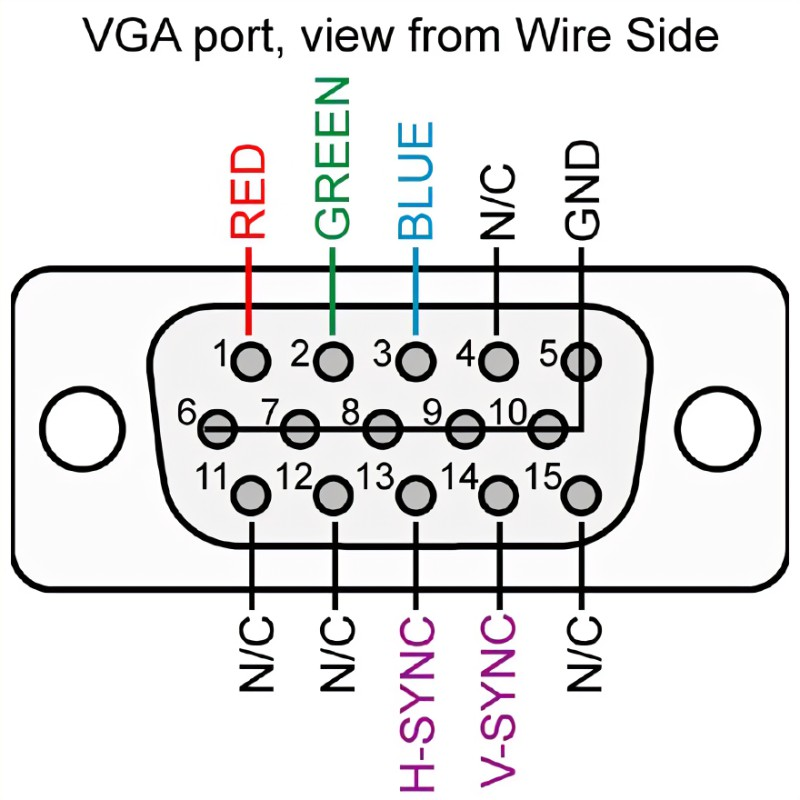
\includegraphics[width=\linewidth]{vga}
    \end{center}
\end{minipage}%
\begin{minipage}[t]{0.5\textwidth}
    \textbf{Signal Overview:}
    \begin{itemize}
        \item \textbf{Red, Green, Blue (RGB):} Analog signals for color intensity.
        \item \textbf{Horizontal Sync (HSYNC):} Synchronizes horizontal lines.
        \item \textbf{Vertical Sync (VSYNC):} Synchronizes vertical frames.
        \item \textbf{Analog Grounds:} Reference points for signals.
    \end{itemize}
\end{minipage}


\subsection*{Algorithm for Displaying an Image using VGA}

To display an image using the VGA protocol, the following steps are typically involved:

\begin{enumerate}
    \item \textbf{Initialize VGA Controller:} Set up registers for resolution, color depth, and synchronization timings.
    
    \item \textbf{Generate Horizontal Sync Signal (HSYNC):} Send pulses to synchronize the start of each line.
    
    \item \textbf{Generate Vertical Sync Signal (VSYNC):} Send pulses to synchronize the start of each frame.
    
    \item \textbf{Output RGB Signals:} For each pixel in the image:
    \begin{itemize}
        \item Calculate appropriate RGB voltages based on the color information of the pixel.
        \item Output analog signals through the corresponding RGB pins.
    \end{itemize}
    
    \item \textbf{Repeat for Each Frame:} Continuously update the screen by repeating the above steps for each frame.
\end{enumerate}


\pagebreak  

\subsection*{OpenGL: Revolutionizing Graphics Rendering}

% \noindent
% \begin{minipage}[t]{0.6\textwidth}
% The development of OpenGL (Open Graphics Library) transformed computer graphics by providing a standardized, cross-platform API for rendering 2D and 3D graphics. Initially developed by Silicon Graphics Inc. (SGI), OpenGL adopted a streamlined pipeline architecture for processing graphical data. The pipeline includes stages for vertex processing, primitive assembly, rasterization, and fragment processing. Each stage optimizes rendering tasks, leveraging hardware acceleration to achieve real-time visual output. OpenGL's versatility and efficiency have made it a cornerstone for interactive applications, ranging from video games to scientific simulations.
% \end{minipage}%
% \begin{minipage}[t]{0.25 \textwidth}
%     \vspace{2pt} % Ensure baseline alignment
%     % \centering
%     \begin{center}
%       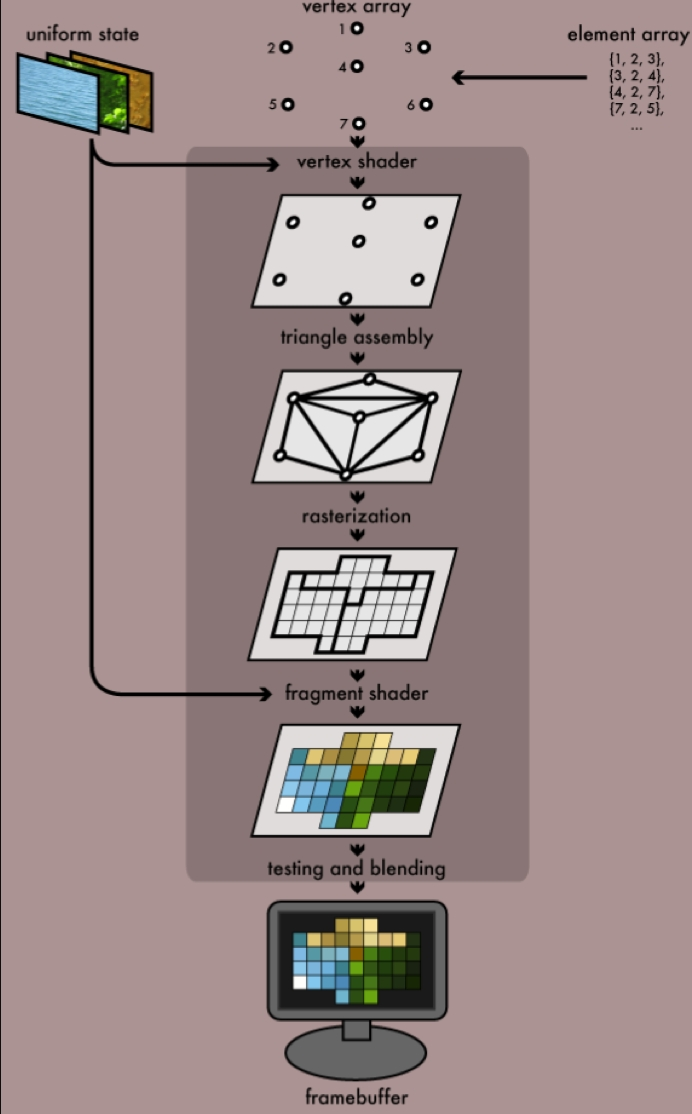
\includegraphics[width=\linewidth]{opengl_pipeline}
%     \end{center}
% \end{minipage}






% \subsection*{Hardware Acceleration and GPU Evolution}
% As demands for graphical complexity grew, dedicated Graphics Processing Units (GPUs) emerged to offload intensive rendering tasks from the CPU. GPUs specialize in parallel processing and include dedicated memory and computational units optimized for graphics operations. This shift enabled real-time rendering of complex scenes with dynamic lighting, textures, and effects. Modern GPUs continue to advance, incorporating technologies like ray tracing and tensor cores for enhanced realism and machine learning applications.


          





\begin{quote}
The rendering engine is built on top of OpenGL, which adheres to the PHIGS standard. In the following, we will explore what PHIGS represents.
\end{quote}

\subsection*{PHIGS}

\textbf{Structure Definition}
\[
\text{Structure } S = \{e_1, e_2, \ldots, e_n \}
\]
\[
\text{where } e_i \in \{\text{Primitive}, \text{Attribute}, \text{Reference to another structure} \}
\]

\textbf{Structure Store Definition}
\[
\text{Structure Store } SS = \{(ID_1, S_1), (ID_2, S_2), \ldots, (ID_m, S_m)\}
\]
\[
\text{where } ID_i \text{ is the identifier of structure } S_i
\]

\textbf{Workstation Definition}
\[
\text{Workstation } W : SS \rightarrow \text{Rendered Image}
\]

\textbf{Output Primitives Definitions}
\[
\text{Point } P = (x, y)
\]
\[
\text{Line } L = \{P_1, P_2\} = \{(x_1, y_1), (x_2, y_2)\}
\]
\[
\text{Polygon } G = \{P_1, P_2, \ldots, P_k\} = \{(x_1, y_1), (x_2, y_2), \ldots, (x_k, y_k)\}
\]
\[
\text{Text } T = (P, \text{string}) = ((x, y), \text{string})
\]

\textbf{Interaction Example}
% \[
% \text{User Input} \rightarrow S_i
% \]
% \[
% SS \cup \{(ID_i, S_i)\} \rightarrow SS'
% \]
% \[
% W(SS') \rightarrow \text{Rendered Image}
% \]
\begin{lstlisting}
// Define a structure with primitives
structure_id = 1;
open_structure(structure_id);
add_primitive(POINT, {x: 10, y: 20});
add_primitive(LINE, {start: {x: 0, y: 0}, end: {x: 100, y: 100}});
close_structure(structure_id);

// Update structure store
structure_store.add({id: structure_id, structure: structure});

// Render on workstation
workstation.render(structure_store);
\end{lstlisting}










          \pagebreak


      \section*{Game Engines}
\addcontentsline{toc}{section}{Game Engines}
          








% \subsection*{Formal Definition}
%   

% \begin{center}
% \begin{math}
%   Let \qquad \qquad S \qquad \qquad \in \quad \{Software Entities\} 
% \end{math}

% \begin{math}
% \qquad \qquad \qquad \qquad \qquad isGameEngine(S) \qquad \qquad 
% \rightleftharpoons \ \ \ isFramework(S) \land (\{S.components\} \subseteq GE::E)
% \end{math}

% \begin{equation} 
%  \qquad \qquad \qquad \qquad \qquad \qquad GE::E \qquad \qquad \qquad 
%  = 
%  \bigcup_{G_i \in GameEngines} \{(G_i, C_j) \mid C_j \in \{G_i.components\}\}
% \end{equation}

% \begin{equation}
% isFramework(S) \qquad
% \rightleftharpoons
% |\{S.components\}| \geq 0 
% \end{equation}

% \end{center}





% \subsection*{Natural Language Understanding}

% \paragraph*{Wikipedia}
% "A game engine is a \textbf{software framework} primarily designed for the development of video games and generally \textbf{includes relevant engines}."






Game engines are comprehensive software frameworks designed for the development and creation of video games. They provide essential tools and libraries for rendering graphics, processing physics, managing assets, and scripting game logic, allowing developers to focus on creating engaging and immersive experiences. A robust game engine is integral to the efficiency and success of game development projects.

\subsection*{Key Features of Game Engines}

\subsubsection*{Rendering Engine}
The rendering engine is responsible for drawing graphics on the screen, handling everything from 2D sprites to complex 3D environments. Advanced rendering engines support features such as lighting, shading, reflections, and particle effects to create visually stunning scenes.

\subsubsection*{Physics Engine}
The physics engine simulates real-world physics to provide realistic movement and interactions between objects in the game world. This includes collision detection, rigid body dynamics, fluid dynamics, and soft body physics.

\subsubsection*{Scripting and AI}
Scripting languages and AI systems are crucial for defining game behavior, character actions, and non-player character (NPC) intelligence. They allow developers to create complex interactions and behaviors without deep programming knowledge.

\subsubsection*{Audio Engine}
The audio engine manages sound effects, music, and voice acting, ensuring they are synchronized with the gameplay and enhance the overall immersive experience.

\subsubsection*{Asset Management}
Efficient asset management tools within the game engine help organize, store, and retrieve game assets such as textures, models, animations, and sounds. This is essential for maintaining a smooth workflow and ensuring all assets are readily accessible.


\pagebreak

\section*{Licensing and Intellectual Property}

Developing a game engine involves critical licensing and intellectual property (IP) considerations. Ensuring compliance with licenses for third-party libraries, assets, and tools, as well as protecting proprietary components, is essential to avoid infringement and unauthorized use.

\subsection*{Open Software vs. Closed Software}

\subsubsection*{Open Software}

Open-source software, such as P5.js, provides publicly available source code that can be freely used, modified, and distributed. This fosters a collaborative and innovative community, encouraging learning and experimentation across various fields.

\subsubsection*{Closed Software}

Proprietary software, like Rockstar's RAGE engine used in the Grand Theft Auto series, restricts access to its source code and limits its use, modification, and distribution. This ensures that Rockstar retains exclusive rights and maintains a competitive edge.

\begin{figure}[h]
    \centering
    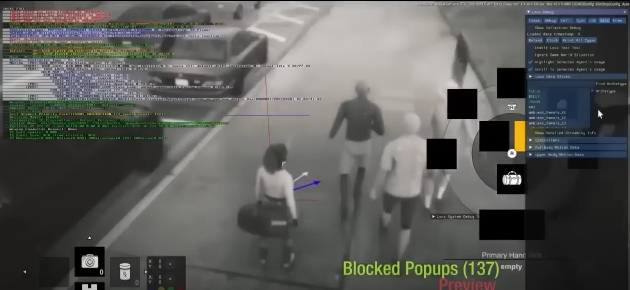
\includegraphics[height=0.4\textwidth]{rage_vector_math}
    \caption{Vectorial Math in RAGE Engine}
\end{figure}

\subsubsection*{Hybrid Models}

Unity represents a hybrid model, offering a free version with basic features and an open API, while advanced features require paid licenses. This approach balances accessibility with commercial viability, supporting widespread use and continuous innovation.

\subsection*{Open Software in this Project}

This project embraces open-source principles, making the game engine's source code publicly available to foster innovation and customization. This openness enhances the engine's versatility and encourages a community of contributors to drive its evolution.


          \pagebreak

          % \fancyhead[L]{GAME ENGINES}
          % \fancyhead[C]{}
          % \fancyhead[R]{}
          % 













          % 




















          % \input{src/content/gameEngine/Unity}
          % \input{src/content/gameEngine/p5.js}
          % \fancyhead[L]{GAME ENGINES}
          % \fancyhead[C]{Problem}
          % \fancyhead[R]{MACHINE LEARNING}
\addcontentsline{toc}{section}{Machine Learning Integration}
          






\subsection*{Machine Learning Integration}

It is common for companies to develop their own in-house game engines and subsequently build their applications on these platforms. However, the integration of pre-installed machine learning components is less prevalent.

Typically, integrating machine learning into games involves installing complex extensions over pre-existing game engines.

\subsubsection*{inWorld AI}
InWorld AI is an example of such a service. It provides installable extensions for popular game engines and offers an interface for communicating with pre-trained OpenAI agents. This solution is excellent for facilitating human-to-AI communication, making it ideal for dialogues and NPC integration.

\begin{figure}[h]
\centering
\begin{minipage}[t]{0.48\textwidth}
\centering
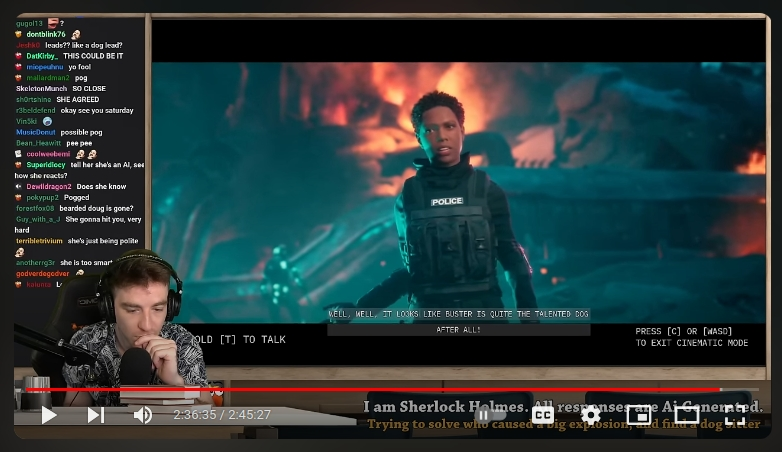
\includegraphics[width=\textwidth, height=5cm]{dougdoug}
\caption{inWorld Ai Demo}
\end{minipage}%
\hfill
\begin{minipage}[t]{0.48\textwidth}
\centering
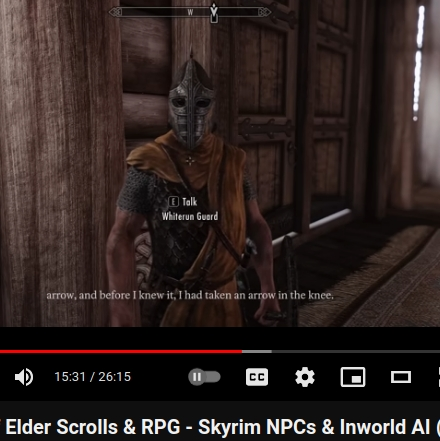
\includegraphics[width=\textwidth, height=5cm]{arrow.jpeg}
\caption{inWorld Ai Demo}
\end{minipage}
\end{figure}

\subsubsection*{Interactive Simulacra of Human Behavior}

Another notable example is this research paper that successfully trained multiple ML agents to interact within a pre-created world. These agents are capable of remembering conversations and interactions and can even organize activities amongst themselves.

\begin{figure}[h]
    \centering
    \begin{minipage}[t]{0.48\textwidth}
        \centering
        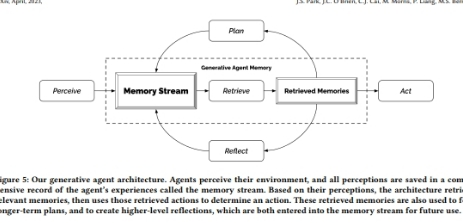
\includegraphics[height= 0.5 \textwidth]{DataStructure.jpeg}
        \caption{Data structure used for memory management}
        % \label{fig:image1}
    \end{minipage}%
    \hfill
    \begin{minipage}[t]{0.48\textwidth}
        \centering
        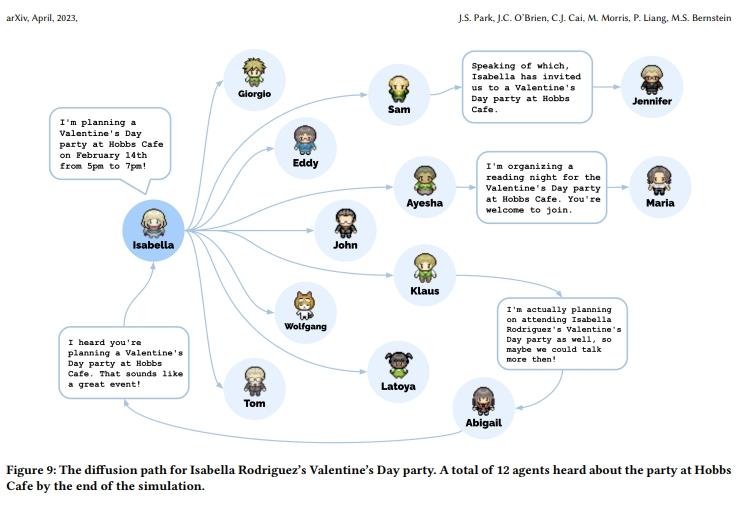
\includegraphics[height= 0.5 \textwidth]{birthdayParty.jpeg}
        \caption{One Agent organised a birthday party}
        % \label{fig:image2}
    \end{minipage}
\end{figure}


By integrating these advanced machine learning solutions, game developers can significantly enhance the immersion and interactivity of their NPCs, creating more engaging and dynamic gameplay experiences.

          \pagebreak

          % \fancyhead[L]{GAME ENGINES}
          % \fancyhead[C]{Solution}
          % \fancyhead[R]{MACHINE LEARNING}
          





To address the absence of game engines with inherent machine learning capabilities, 
I propose the development of a new game engine designed from the ground up with ML integration as a core feature. 
This engine will enable developers to create more immersive and interactive experiences by seamlessly incorporating machine learning into their game development process.

\subsection*{Key Features of the Proposed Game Engine}

\begin{itemize}
    \item \textbf{Built-In Machine Learning Frameworks:}
    \begin{itemize}
        \item The engine will come pre-integrated with popular machine learning libraries such as TensorFlow, PyTorch, and OpenAI's GPT. 
This eliminates the need for complex extensions and allows developers to leverage ML capabilities directly within the engine.
    \end{itemize}
    
    \item \textbf{Easy Integration with Existing ML Models:}
    \begin{itemize}
        \item Developers will be able to import pre-trained models easily and use them to enhance NPC behaviors, generate dynamic content, and more. This feature streamlines the process of integrating sophisticated AI into games.
    \end{itemize}
    
    \item \textbf{Real-Time Learning and Adaptation:}
    \begin{itemize}
        \item The engine will support real-time learning, enabling game entities to adapt based on player interactions. This creates a more dynamic and responsive game environment.
    \end{itemize}
    
    \item \textbf{Voice Interaction Capabilities:}
    \begin{itemize}
        \item With built-in support for microphone input, developers can create NPCs that engage in live dialogue with players, enhancing the realism and immersion of the game.
    \end{itemize}
    
    \item \textbf{Compatibility with Popular Game Development Practices:}
    \begin{itemize}
        \item Drawing inspiration from industry-leading platforms like Unity and p5.js, the engine will offer a user-friendly interface and robust documentation. This ensures that developers can transition smoothly to using the new engine without a steep learning curve.
    \end{itemize}
\end{itemize}


\subsection*{Benefits of the Proposed Solution}

\begin{itemize}
    \item \textbf{Enhanced Immersion:}
    \begin{itemize}
        \item By integrating machine learning, games can offer more lifelike and unpredictable NPC behaviors, creating a richer player experience.
    \end{itemize}
    
    \item \textbf{Dynamic Content Generation:}
    \begin{itemize}
        \item The engine will enable the creation of content that evolves based on player actions, providing a unique and personalized gaming experience.
    \end{itemize}
    
    % \item \textbf{Streamlined Development Process:}
    % \begin{itemize}
    %     \item Built-in ML capabilities mean developers spend less time configuring external libraries and more time focusing on game design and mechanics.
    % \end{itemize}
    % 
    % \item \textbf{Broad Accessibility:}
    % \begin{itemize}
    %     \item The user-friendly design ensures that a wide range of developers, from indie creators to large studios, can utilize the engine effectively.
    % \end{itemize}
\end{itemize}



% \begin{lstlisting}
% void start();
% void update();
% int main() { Awake(); }
% void Awake() {
%   RenderEngine::setStart(start);
%   RenderEngine::setUpdate(update);
%   RenderEngine::setFixedUpdate(fixedUpdate);
%   // MUST BE CALLED LAST
%   RenderEngine::START(true);
% }
% void start() {
%   Gameobject go; int speed = 0.01;
%   Debug::Log(go.transform.name)
%   Debug::Log(go.transform.position)
%   
%   go.transform.translate(Vector3::Right * speed)
%   Debug::Log(go.transform.position)
%   go.transform.position = Vector3::one * Math::sqrt(Math::pi);
%   Debug::Log(go.transform.position)
% }
% \end{lstlisting}












          \pagebreak
          % \fancyhead[L]{COMPUTER GRAPHICS}
          % \fancyhead[C]{History}
          % \fancyhead[R]{GAME ENGINES} 
          % 
\subsection*{From RGB LEDs to VGA}
\begin{itemize}
    \item \textbf{RGB LED:} Basic color representation with \( R, G, B \) channels.
    \item \textbf{VGA Protocol:} Standard for analog video output from computers.
\end{itemize}

\subsection*{Communicating with VGA Protocol}

The VGA protocol is implemented using various pins on a connector. It supports several analog signals for color and synchronization. Here's a simplified overview:

\begin{minipage}[t]{0.5\textwidth}
    \textbf{Pinout Diagram:}
    \begin{center}
        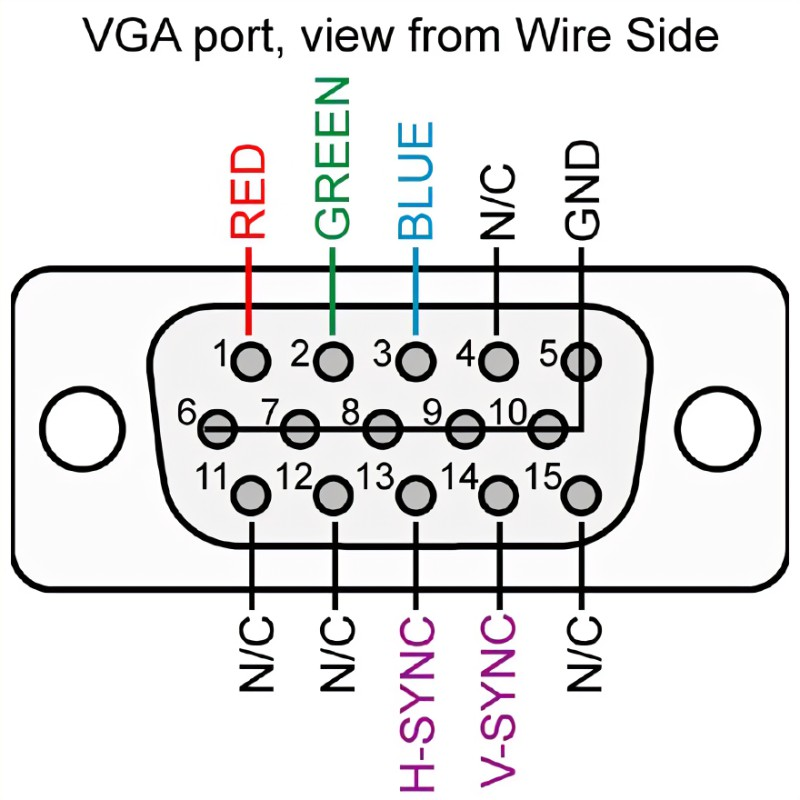
\includegraphics[width=\linewidth]{vga}
    \end{center}
\end{minipage}%
\begin{minipage}[t]{0.5\textwidth}
    \textbf{Signal Overview:}
    \begin{itemize}
        \item \textbf{Red, Green, Blue (RGB):} Analog signals for color intensity.
        \item \textbf{Horizontal Sync (HSYNC):} Synchronizes horizontal lines.
        \item \textbf{Vertical Sync (VSYNC):} Synchronizes vertical frames.
        \item \textbf{Analog Grounds:} Reference points for signals.
    \end{itemize}
\end{minipage}


\subsection*{Algorithm for Displaying an Image using VGA}

To display an image using the VGA protocol, the following steps are typically involved:

\begin{enumerate}
    \item \textbf{Initialize VGA Controller:} Set up registers for resolution, color depth, and synchronization timings.
    
    \item \textbf{Generate Horizontal Sync Signal (HSYNC):} Send pulses to synchronize the start of each line.
    
    \item \textbf{Generate Vertical Sync Signal (VSYNC):} Send pulses to synchronize the start of each frame.
    
    \item \textbf{Output RGB Signals:} For each pixel in the image:
    \begin{itemize}
        \item Calculate appropriate RGB voltages based on the color information of the pixel.
        \item Output analog signals through the corresponding RGB pins.
    \end{itemize}
    
    \item \textbf{Repeat for Each Frame:} Continuously update the screen by repeating the above steps for each frame.
\end{enumerate}


\pagebreak  

\subsection*{OpenGL: Revolutionizing Graphics Rendering}

% \noindent
% \begin{minipage}[t]{0.6\textwidth}
% The development of OpenGL (Open Graphics Library) transformed computer graphics by providing a standardized, cross-platform API for rendering 2D and 3D graphics. Initially developed by Silicon Graphics Inc. (SGI), OpenGL adopted a streamlined pipeline architecture for processing graphical data. The pipeline includes stages for vertex processing, primitive assembly, rasterization, and fragment processing. Each stage optimizes rendering tasks, leveraging hardware acceleration to achieve real-time visual output. OpenGL's versatility and efficiency have made it a cornerstone for interactive applications, ranging from video games to scientific simulations.
% \end{minipage}%
% \begin{minipage}[t]{0.25 \textwidth}
%     \vspace{2pt} % Ensure baseline alignment
%     % \centering
%     \begin{center}
%       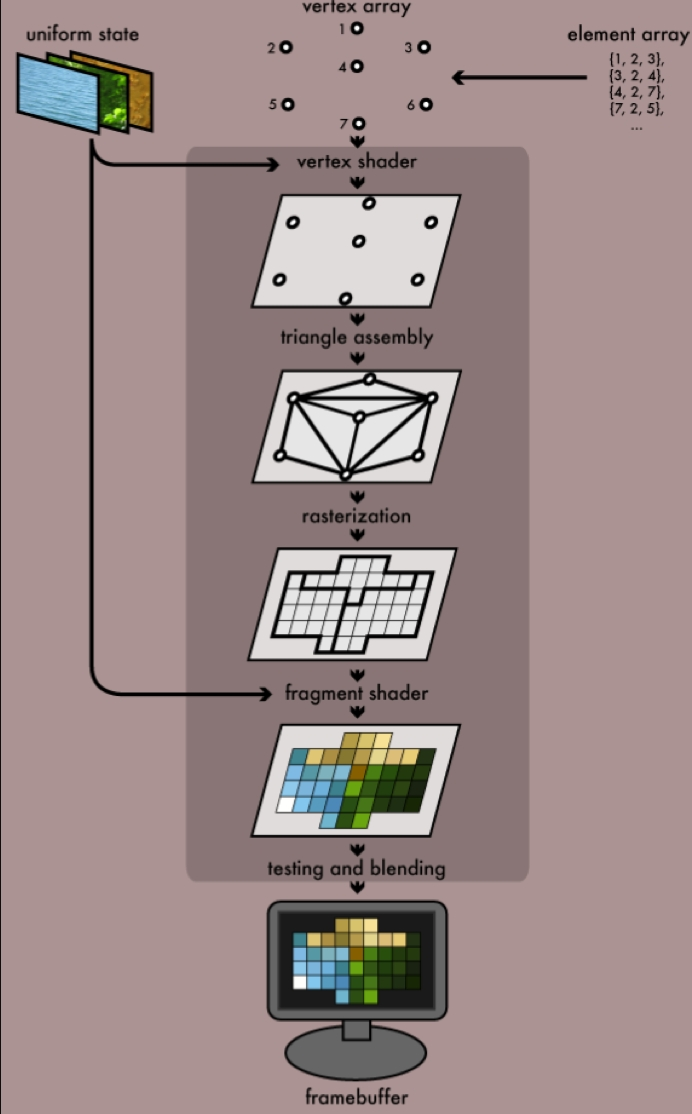
\includegraphics[width=\linewidth]{opengl_pipeline}
%     \end{center}
% \end{minipage}






% \subsection*{Hardware Acceleration and GPU Evolution}
% As demands for graphical complexity grew, dedicated Graphics Processing Units (GPUs) emerged to offload intensive rendering tasks from the CPU. GPUs specialize in parallel processing and include dedicated memory and computational units optimized for graphics operations. This shift enabled real-time rendering of complex scenes with dynamic lighting, textures, and effects. Modern GPUs continue to advance, incorporating technologies like ray tracing and tensor cores for enhanced realism and machine learning applications.



          % \input{src/content/gameEngine/openSoftware}
          % 







% In this section, we will inspect the criteria to which a piece of software needs to qualify in order to be considered part of the game engines set.


\begin{center}
\subsection*{Formal Proof}
\textbf{Creation of GG}

\begin{math}
&\text{Let } GG \text{ be the thesis project game engine with } GG.\text{components} = \{M, R, E, FM\}.
\end{math}

\begin{math}
&\text{We know that } \exists Unity \in GameEngines
\end{math}

\begin{math}
Unity.components = \{  \}
\end{math}

More in-depth analysis of Unity's components is done in Field Study chapter.
Right now, we are only interested in the Vector3 and Transform Classes.


\subsubsection*{Demonstration with Unity}

\begin{equation}
\begin{aligned}
&\text{Let Unity be a well-known game engine.} \\
&\text{Unity also includes components } \{M, R, E, FM\}. \\
&\text{Therefore, } \text{isGameEngine(Unity)}.
\end{aligned}
\end{equation}
\end{center}



\subsection*{Formal Conclusion}

\begin{math}
GG \overset{\text{DEFAULT}}{\subseteq} \text{SoftwareEntities} 
\end{math}

\begin{math}
GG \overset{|GG.components| \geq 0}{\subseteq} \text{Frameworks} 
\end{math}

\begin{math}
GG \overset{|GG.components| \geq 0}{\subseteq} \text{GameEngines} 
\end{math}











\begin{equation}
\begin{align}

\label{}
\end{align}
\end{equation}

Let \( S \) be a piece of software, input for a function \( \text{isGameEngine} \) that outputs a binary response.
\[
\text{isGameEngine}(S) = \text{isFramework}(S) \land (\text{S::Components} \subseteq \text{GE::E})
\]


\begin{equation} \label{FrameworkDef}
\begin{align*} 
&GG \in \text{SoftwareFrameworks} 
\rightleftharpoons
&|GG::\text{Components}| \geq 0 
\end{align*}
\end{equation}


where \(\text{GE::E}\) represents the collection of \forall \text{components in } \forall \text{game engines, formulated as:}
\]
\begin{equation} \label{gameEngineDef}
  \text{GE::E} = \bigcup_{G \in \text{GameEngines}} \{(G, C) \mid C \in \text{Components}\}
\end{equation}

\begin{equation} \label{myGameEngineDef}
\begin{align*} 
&\text{Let } GG \in \text{Piece of Software} \\
&\text{Let } GG::\text{Components} = \{M, R, E, FM\}
\end{align*}
\end{equation}


\begin{equation} \label{isGGaGE}
\begin{align*} 
&GG \in \text{GameEngines} 
\rightleftharpoons
&GG::\text{Components} \subseteq \text{GE::E}
\end{align*}
\end{equation}




% \begin{subequation} 
% &GG::M, GG::R, G::E, G::FM \in \text{Components}
% \rightleftharpoons



\text{ denote MathEngine, RendererEngine,
GUI Editor, and File Manager respectively.} \\
\end{subequation}












% \textbf{Given:}
% \begin{equation}
% \begin{aligned}
% &M, R, GUI, FM \text{ denote MathEngine, RendererEngine, GUI Editor, and File Manager respectively.}
% \end{aligned}
% \end{equation}

% \textbf{Statement 1:}
\begin{equation}
\begin{center}
  (&(\exists GG) . \text{isGameEngine}(GG))
  \land

  \land 
  (\text{GG::Components} = \{M, R, GUI, FM\}) \\

&\land (\exists G_i) \, \text{isGameEngine}(G_i) \land (\text{G_i::Components} = \{M, R, GUI, FM\}) \\

&\Rightarrow \text{isGameEngine}(GG)
\end{center}
\end{equation}

\textbf{Statement 2:}
\begin{equation}
\begin{aligned}
&(\exists \text{ Unity}) \, \text{isGameEngine(Unity)} \land (\text{Unity::Components} = \{M, R, GUI, FM\})
\end{aligned}
\end{equation}

\textbf{Proof:}

% \textbf{Statement 1 Proof:}
\begin{equation}
% \begin{aligned}
&\text{Let } GG \text{ and } G_i \text{ be such that } \\
&\text{isGameEngine}(GG) \land (\text{GG::Components} = \{M, R, GUI, FM\}), \\
&\text{isGameEngine}(G_i) \land (\text{G_i::Components} = \{M, R, GUI, FM\}). \\
&\text{Therefore, } \text{isGameEngine}(GG).
% \end{aligned}
\end{equation}

\textbf{Statement 2 Proof:}
\begin{equation}
\begin{aligned}
&\text{Let Unity be such that } \text{isGameEngine(Unity)} \land (\text{Unity::Components} = \{M, R, GUI, FM\}).
\end{aligned}
\end{equation}








\noindent\rule{\linewidth}{0.4pt}


In mathematical notation, the usage of specific game engines in different scenarios can be represented as:

\[
\begin{aligned}
&\text{UnrealEngine} \in \text{PhotoRealisticScenarios} \\
&\text{Unity} \in \text{ClothSimulators} \\
&\text{P5.js} \in \text{PhysicsDemonstrations}
\end{aligned}
\]

\noindent\rule{\linewidth}{0.4pt}

\textbf{Given:}
\begin{align*}
&\text{Let } ME, RE, GUIE, FM \text{ denote MathEngine, RendererEngine, GUI Editor, and File Manager respectively.} \\
&\text{From the code snippets:} \\
&\text{isGameEngine}(ME) \Rightarrow \text{isFramework}(ME) \land (\text{ME::Components} \subseteq \text{GE::E}) \\
&\text{isGameEngine}(RE) \Rightarrow \text{isFramework}(RE) \land (\text{RE::Components} \subseteq \text{GE::E}) \\
&\text{isGameEngine}(GUIE) \Rightarrow \text{isFramework}(GUIE) \land (\text{GUIE::Components} \subseteq \text{GE::E}) \\
&\text{isGameEngine}(FM) \Rightarrow \text{isFramework}(FM) \land (\text{FM::Components} \subseteq \text{GE::E}) \\
\end{align*}

\textbf{To Prove:}
\[
\text{Using or building game engines } GE \text{ is standard industry practice.}
\]

\textbf{Proof:}
\begin{align*}
&\text{Each engine (MathEngine, RendererEngine, GUI Editor, File Manager) is considered a game engine if it satisfies} \\
&\text{the criteria } \text{isGameEngine}(S) \Rightarrow \text{isFramework}(S) \land (\text{S::Components} \subseteq \text{GE::E}). \\
&\text{These engines demonstrate specialized functionalities essential for gaming and diverse applications,} \\
&\text{such as mathematical computations, rendering graphics, user interface design, and file management.} \\
&\text{Their existence and usage across industries highlight the necessity and ubiquity of game engines,} \\
&\text{thus establishing the practice of using or building them as standard in the industry.}
\end{align*}


















          % 




subsection*{Natural Language Understanding}

\paragraph*{Wikipedia}
"A game engine is a software framework primarily designed for the development of video games and generally includes relevant engines."



\subsection*{Formal Definition}
  Let \( S \) be a piece of software, input for a function \( isGameEngine \) that outputs a binary response. 
 \[
    \text{isGameEngine} (\text{Software } S) =
    \text{isFramework}(S) \land (\text{S::Components} \subseteq \text{GE::E})
\] 

  where GameEngine::Engines
  represents the collection of all possible engines in all possible game engines, as such:
  \[
  \text{GE::E} = 
  \[
    \{
      ...
    \text{Render}, 
    \text{Script}, 
    \text{Physics}, 
    \text{AI}, 
    \text{SFX}, 
    \text{Robotics}
    ...
   \}
  \end{cases}
  \]























    % \fancyhead[C]{demo}

    





    \begin{center}
    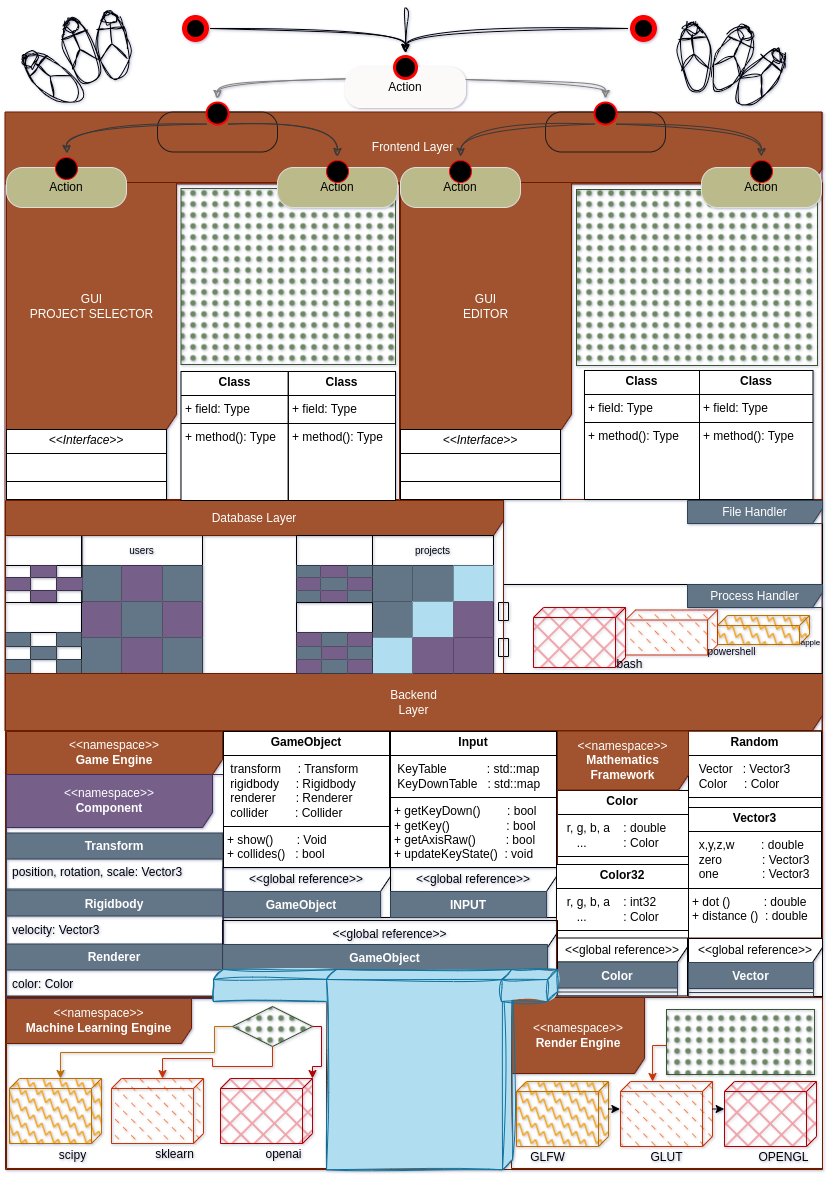
\includegraphics[width=1 \textwidth]{app_arch.png}
    \end{center}







    \part{Implementation}
    \fancyhead[L]{GAME ENGINE} % clear all footer fields
    \fancyhead[R]{IMPLEMENTATION} % clear all footer fields
    \fancyhead[C]{Results}
        


\subsection*{Results}

\begin{lstlisting}[caption={DVD\_Logo\_Bouncer Example Code}]
#include "../../engine/engine.h"  
int main()
{
  RenderEngine::setStart(start); RenderEngine::setUpdate(update); RenderEngine::Enabled(true);
}
GameObject dvd; GameObject vWalls[2]; GameObject hWalls[2];
void start()
{
  dvd.rigidbody.velocity = Vector3(0.01, 0.001);

  vWalls[0].transform.position = Vector3(-1, 0); vWalls[0].transform.scale = Vector3(0.01, 2);
  ...
  hWalls[1].transform.position = Vector3(0, 1); hWalls[1].transform.scale = Vector3(2, 0.01);
}
void update()
{
  RenderEngine::background(0);
  dvd.transform.position += dvd.rigidbody.velocity;
  dvd.show();
  for (GameObject& wall : vWalls)
    if(dvd.collides(wall)) 
      dvd.rigidbody.velocity.x = -dvd.rigidbody.velocity.x;

  for (GameObject& wall : hWalls)
    if(dvd.collides(wall)) 
      dvd.rigidbody.velocity.y = -dvd.rigidbody.velocity.y;

  if(GameEngine::Input::getKeyDown(GameEngine::KEY_R))
    dvd.transform.position = Vector3::zero;
}
\end{lstlisting}

\subsection*{Analysis}

\begin{minipage}[t]{0.5\linewidth}
    \textbf{start Function Description:}
    \begin{itemize}
        \item \textbf{DVD Velocity:} $(0.01, 0.001)$
        \item \textbf{Vertical Walls:}
        \begin{itemize}
            \item Left: $(-1, 0)$
            \item Right: $(1, 0)$
        \end{itemize}
        \item \textbf{Horizontal Walls:}
        \begin{itemize}
            \item Bottom: $(0, -1)$
            \item Top: $(0, 1)$
        \end{itemize}
    \end{itemize}
\end{minipage}%
\begin{minipage}[t]{0.5\linewidth}
    \textbf{update Function Description:}
    \begin{itemize}
        \item \textbf{Collision Detection:}
        \begin{itemize}
            \item Let $A$ and $B$ be two axis-aligned squares with:
            \begin{itemize}
                \item Center of $A$: $(x_A, y_A)$, Side length: $s_A$
                \item Center of $B$: $(x_B, y_B)$, Side length: $s_B$
            \end{itemize}
            \item Collision occurs if:
            \[
            (x_A - x_B)^2 + (y_A - y_B)^2 \leq \left(\frac{s_A + s_B}{2}\right)^2
            \]
        \end{itemize}
    \end{itemize}
\end{minipage}




        


\begin{center}
  \underline{\textbf{Each Game Engine has its own style based by its functionality}}

  \emph{Each Game Engine defines its functionality through its implemented components.}
% , this harmony gives the style.}
\end{center}











        



\subsection*{Sources of Inspiration}

The development of the game engine draws inspiration from several established platforms:

        \textbf{Unity:} The math engine draws inspiration from Unity's advanced mathematical computations and transformations, leading to the development of a robust internal framework.


    % 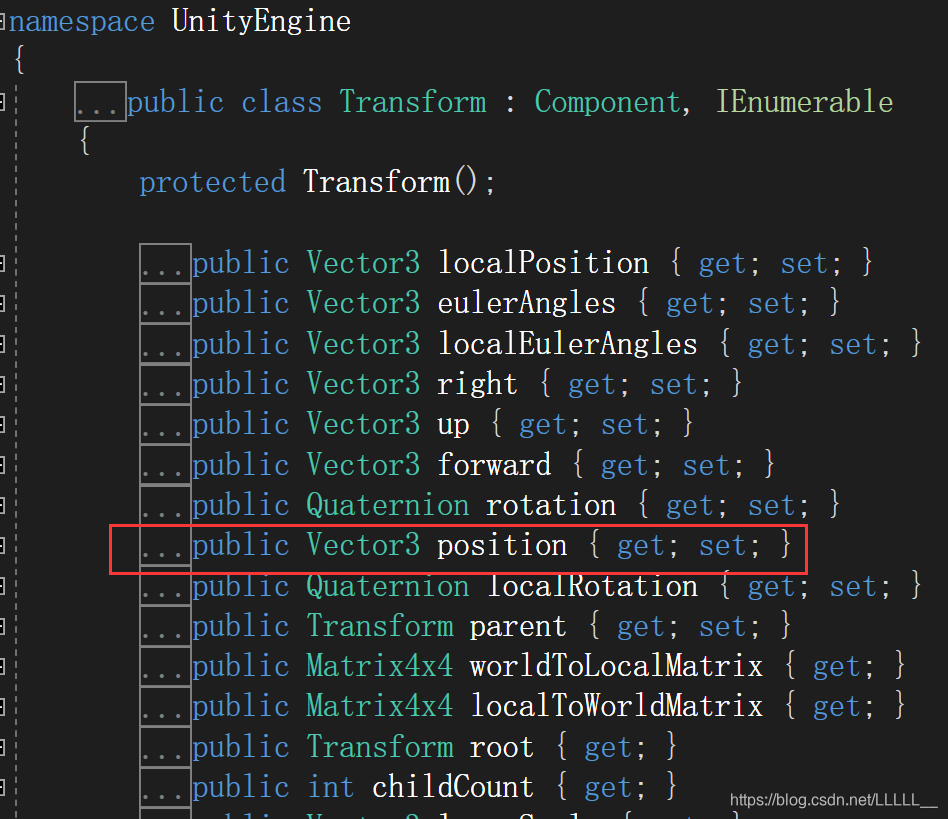
\includegraphics[height=5cm]{unity_transform}
    % \caption*{Unity Transform}

 \begin{lstlisting}
  void start();
  void update();
  int main() { Awake(); }
  void Awake() {
    RenderEngine::setStart(start);
    RenderEngine::setUpdate(update);
    RenderEngine::setFixedUpdate(fixedUpdate);
    // 
    RenderEngine::START(true);
  }
  void start() {
    Gameobject go;
    go.transform.position = Random::Vector3().normalised *  Random::Value(-5, 5); 
    Debug::Log(go.transform.position)
  }
  \end{lstlisting}


% \begin{figure}[htbp]
%     \centering
%     \begin{minipage}[t]{0.4\textwidth}
%         \textbf{Unity:} The math engine is inspired by Unity's robust handling of complex mathematical computations and transformations. Unity's versatility and efficient math libraries have guided the development of our own mathematical framework within the engine.
%     \end{minipage}\hfill
%     \begin{minipage}[t]{0.4\textwidth}
%         \centering
%         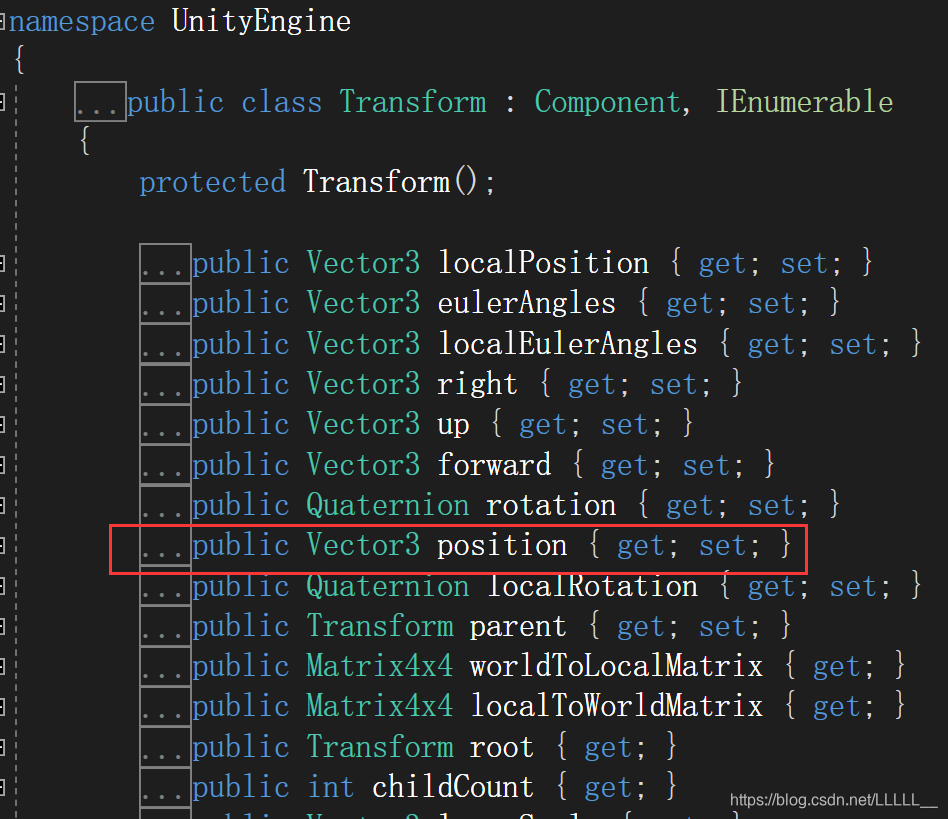
\includegraphics[height=5cm]{unity_transform}
%         \caption*{Unity Transform}
%     \end{minipage}
%     
%     \begin{minipage}{0.45\textwidth}
%         \begin{lstlisting}[language=C++, caption={Example Code}]
% void start();
% void update();
% int main() { Awake(); }
% void Awake() {
%   RenderEngine::setStart(start);
%   RenderEngine::setUpdate(update);
%   RenderEngine::setFixedUpdate(fixedUpdate);
%   // 
%   RenderEngine::START(true);
% }
% void start() {
%   GameObject go;
%   go.transform.position = Random::Vector3().normalized() * Random::Value(-5, 5); 
%   Debug::Log(go.transform.position);
% }
%         \end{lstlisting}
%     \end{minipage}
% \end{figure}


\textbf{p5.js:} The rendering engine draws inspiration from p5.js, renowned for its simplicity and accessibility in the creative coding community. The straightforward approach to rendering and graphical output in p5.js has influenced our rendering pipeline's design, making it powerful and user-friendly.













\begin{lstlisting}

  point(x, y, c); // Changes the color of the pixel at location <x, y> to c

  line(<<x>, <y>>, 
       <<x>, <y>>); // Draws a line between 2 points

  background(color);

  square(point1, point2);
  fill(color);
  noStroke();
  circle(point , radius);

\end{lstlisting}








% \begin{lstlisting}
% void start();
% void update();
% int main() { Awake(); }
% void Awake() {
%   RenderEngine::setStart(start);
%   RenderEngine::setUpdate(update);
%   RenderEngine::setFixedUpdate(fixedUpdate);
%   // MUST BE CALLED LAST
%   RenderEngine::START(true);
% }
% void start() {
%   Gameobject go; int speed = 0.01;
%   Debug::Log(go.transform.name)
%   Debug::Log(go.transform.position)
%   
%   go.transform.translate(Vector3::Right * speed)
%   Debug::Log(go.transform.position)
%   go.transform.position = Vector3::one * Math::sqrt(Math::pi);
%   Debug::Log(go.transform.position)
% }
% \end{lstlisting}










        


\begin{center}
  \underline{\textbf{Each component in a software framework must work in harmony}}

  \emph{Each Game Engine defines its functionality through its implemented components.}
% , this harmony gives the style.}
\end{center}




        \pagebreak
        

  % \begin{center}
  % 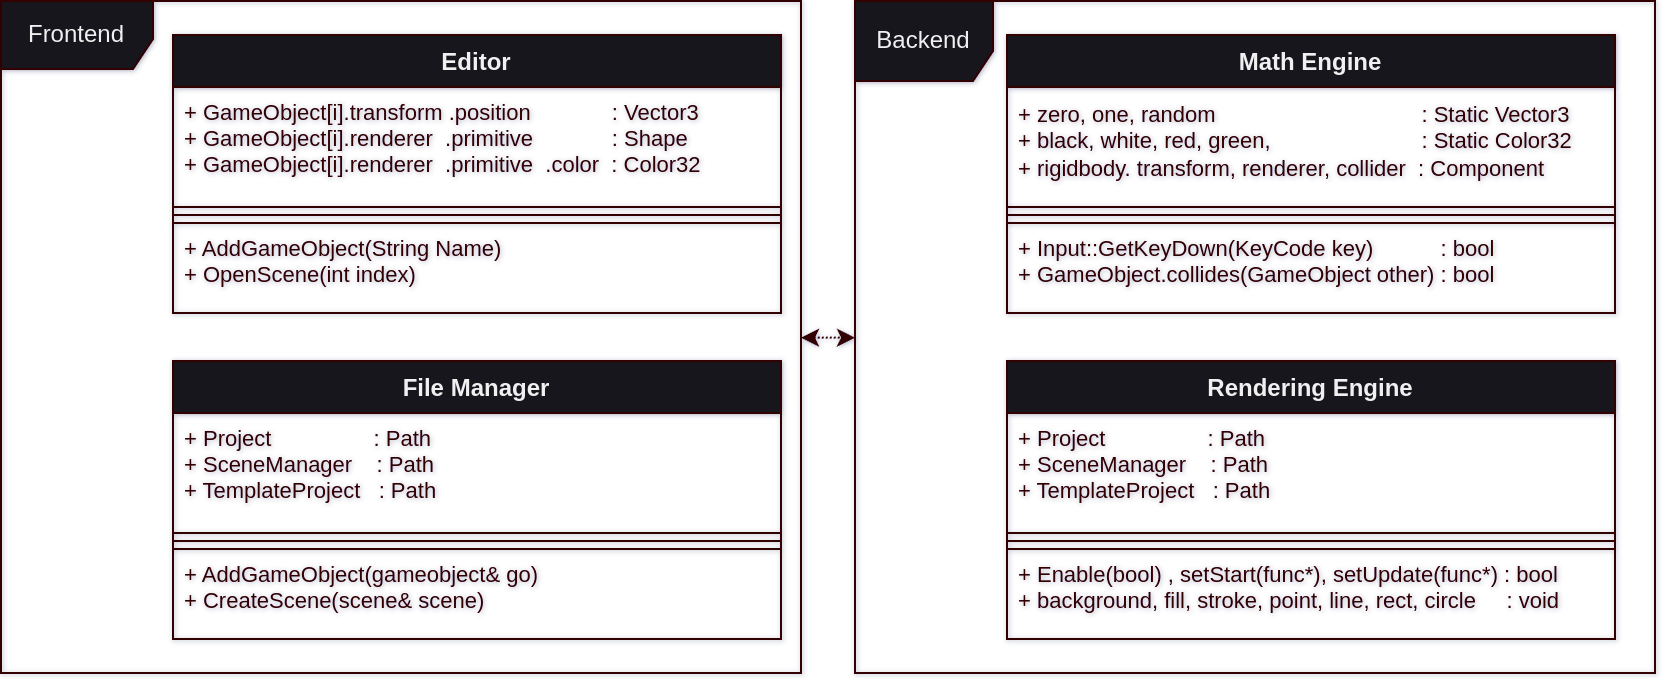
\includegraphics[width=1 \textwidth]{app_overview.png}
  % \end{center}





% \begin{center}
% 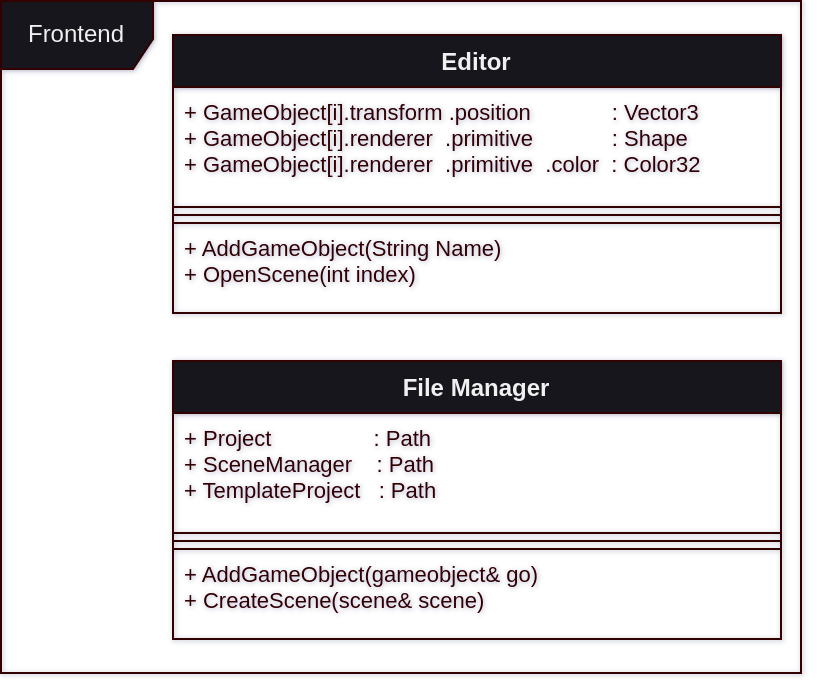
\includegraphics[width=0.486 \textwidth]{app_frontend_overview.png}
% \end{center}


% \begin{center}
% 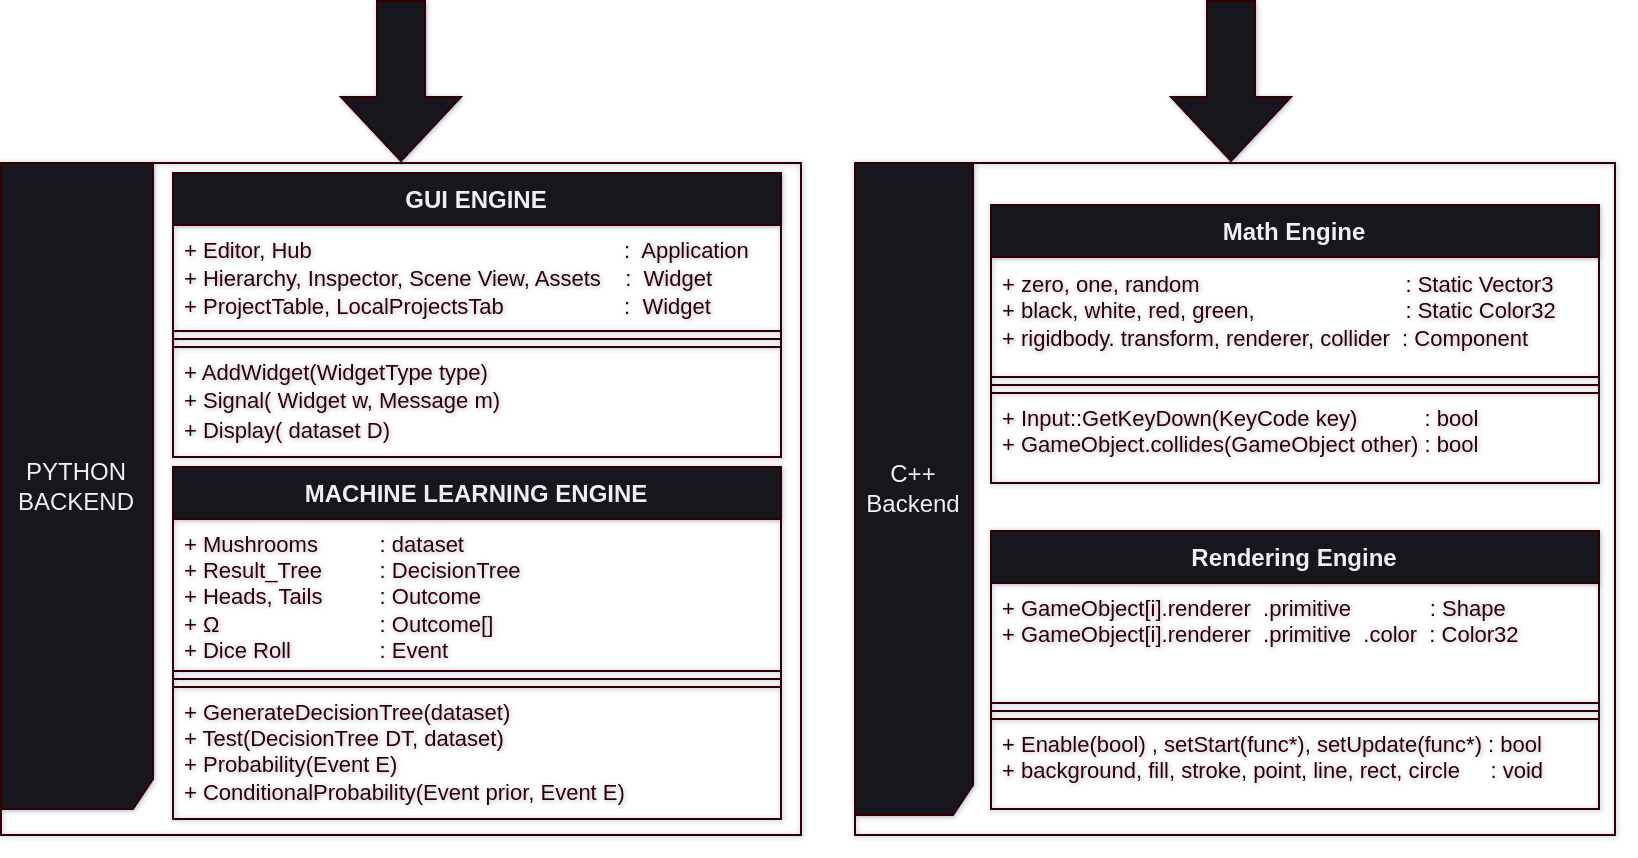
\includegraphics[width=0.9 \textwidth]{app_backend_overview.png}
% \end{center}




% \begin{minipage}[t]{0.45\textwidth}
%     \centering
%     \textbf{Frontend}
%     
%     \begin{tikzpicture}
%         \begin{axis}[
%             axis lines = left,
%             xlabel = $x$,
%             ylabel = {$y=f(x)$},
%         ]
%         \addplot [
%             domain=-10:10, 
%             samples=100, 
%             color=blue,
%         ]
%         {x^2};
%         \end{axis}
%     \end{tikzpicture}
% \end{minipage}
% \hfill
% \begin{minipage}[t]{0.45\textwidth}
%     \centering
%     \textbf{Backend}
%     
%     \begin{equation*}
%         \text{Input: } x = 3
%     \end{equation*}
%     \begin{equation*}
%         y = x^2 = 3^2 = 9
%     \end{equation*}
% \end{minipage}

% \vspace{0.5cm}

% \textbf{Interaction}

% \begin{minipage}[t]{0.3\textwidth}
%     \begin{equation*}
%         \text{Frontend: } \text{Enter } x
%     \end{equation*}
% \end{minipage}
% \begin{minipage}[t]{0.3\textwidth}
%     \begin{equation*}
%         \text{Backend: } y = x^2
%     \end{equation*}
% \end{minipage}
% \begin{minipage}[t]{0.3\textwidth}
%     \begin{equation*}
%         \text{Frontend: } y = 9
%     \end{equation*}
% \end{minipage}

        \pagebreak
        \fancyhead[C]{}
        \fancyhead[L]{GAME ENGINE}
        \section*{The Frontend}
          \fancyhead[R]{COMPONENTS}
          \fancyhead[C]{FRONTEND}
          





\begin{quote}
  The frontend component is organized into several directories and files. It includes functionalities for the editor, hub, and splash interfaces.
  \end{quote}





          

  
  \[
    \text{Directory } D := \{d_1, d_2, \ldots, d_n\}, \quad \text{where } \text{TypeOf}(d_i) \in \{\text{File}, \text{Directory}\}
  \]
  
  \[
    \forall \ module_i \in \text{frontend} \Rightarrow 
    module_i \supseteq \{\text{init.py}, \text{main.py}, \text{cli.py}\}
  \]
  
  Specific to this implementation, we have the following modules and sub-modules:
  
  \[
    (\exists \ \text{Editor} \in \text{Modules}). \ \text{Editor.submodules} \
    \rightarrow_{\text{depend on}} \ \text{PyQt}
  \]
  
  \[
    (\exists \ \text{Editor} \in \text{Modules}). \ \text{Editor.submodules} \
    \supseteq \{\text{Hierarchy}, \text{Scene View}, \text{Inspector}, \text{Assets}, \text{Terminal}\}
  \]
  
  \[
    (\exists \ \text{Assets} \in \text{Editor.submodules}). \ \text{Assets} \rightarrow_{\text{modifies}} \{\text{Project Tree}\} 
  \]
  
  \[
    (\exists \ \text{Hierarchy} \in \text{Editor.submodules}). \ \text{Hierarchy} \rightarrow_{\text{modifies}} \ \text{JSON\_Scene\_File}
  \]
  
  \[
    (\exists \ \text{Inspector} \in \text{Editor.submodules}). \ \text{Inspector} \rightarrow_{\text{modifies}} \ \text{JSON\_Scene\_File}
  \]
  
  The interactions between different modules can be represented using functions and mappings. Let \( f: E \to H \) represent the function mapping elements from the Editor to the Hub. 
  Similarly, \( g: H \to S_p \) represents the mapping from Hub to Splash.
  
  \[
  \begin{aligned}
    \text{user} &\xrightarrow{\text{launch}} \text{splash}     
         \xrightarrow{\text{launch}} \text{Hub}          
         \xrightarrow{\text{launch}} \text{Editor} \\
  \end{aligned}
  \]
 
  \[
  \begin{aligned}
        \text{Editor}  &\xrightarrow{\text{launch}} \{\text{Hierarchy}, \text{SceneView}, \text{Inspector}, \text{Assets}\}
  \end{aligned}
  \]

  \[
  \text{SceneView} \xrightarrow{\text{launch}} (\text{c++ } \land \text{python}) \ \text{Runner} \xrightarrow{\text{launch}} \{\text{opengl}, \text{scipy}\}
  \]
  
  \[
  \text{Hierarchy} \xrightarrow{\text{reads}} \{\text{active\_scene.json}\}
  \]
  
  \[
  \text{Inspector} \xrightarrow{\text{reads}} \{\text{active\_game\_object.json}\}
  \]
  
  \[
  \text{Assets} \xrightarrow{\text{reads}} \{\text{FileTreeOf(projectPath)}\}
  \]
  
  \[
  (\text{user} \land \text{Hub}) \lor (\text{user} \land \text{Editor}) \lor (\text{user} \land \text{CLInterface}) \xrightarrow{\text{Request}} (\text{FileManager} \lor \text{SceneManager})
  \xrightarrow{\text{response}}
  \]
  
  % \[
  % \xrightarrow{\text{request}} (\text{FileManager} \lor \text{SceneManager})
  % \xrightarrow{\text{response}}
  % \]
  % 

% \begin{quote}
% The frontend component is organized 
% into several directories and files. 

% It includes functionalities for 
% the editor, hub, and splash interfaces. 
% \end{quote}


% \begin{math}
%   Directory \ D \ :=  \{d_1, d_2, \ldots, d_n\}
%   , 
%   where \ \ \TypeOf (\( d_i \)) \in \{File, Directory\}
% \end{math}


% \begin{math}
%   \forall module_i \in frontend \Rightarrow 
%   module_i 
%   \supseteq
%   \{init.py, main.py, cli.py\}
% \end{math}

% Specific to this implementation, 
% we have the following modules and sub-modules:


% \begin{math}
%   (\exists \ Editor \in Modules).
%   Editor.submodules \
%   \rightarrow_{depend\ on} PyQt
% \end{math}

% \begin{math}
%   (\exists \ Editor \in Modules).
%   Editor.submodules \
%   \supseteq \{ Hierarchy, Scene \ View, Inspector, Assets, Terminal \}
% \end{math}


% \begin{math}
%   (\exists \ Assets \in Editor.submodules).
%   \ Assets \rightarrow_{modifies} \{ \ Project \ Tree \} 
% \end{math}

% \begin{math}
%   (\exists \ Hierarchy \in Editor.submodules).
%   \ Hierarchy \rightarrow_{modifies} \ JSON\_Scene\_File
% \end{math}

% \begin{math}
%   (\exists \ Inspector \in Editor.submodules).
%   \ Inspector \rightarrow_{modifies} JSON\_Scene\_File\ 
% \end{math}

% % \begin{math}
% %   (\exists \ Terminal \in Editor.submodules).
% %   \ Terminal = Terminal
% % \end{math}



% The interactions between different modules can be represented using functions and mappings.
% Let \( f: E \to H \) represent the function mapping elements from the Editor to the Hub.
% Similarly, \( g: H \to S_p \) represents the mapping from Hub to Splash.


% \begin{math}

%   user \xrightarrow{launch} splash     
%        \xrightarrow{launch} Hub          
%        \xrightarrow{launch} Editor
%        \xrightarrow{launch} \{Hierarchy, SceneView, Inspector, Assets \}

%   SceneView \xrightarrow{launch} (\text{c++ } \land python ) \  Runner \xrightarrow{launch} \{ opengl, matplotlib, numpy \}

%   Hierarchy \xrightarrow{reads} \{ active_scene.json \}
  
%   Inspector \xrightarrow{reads} \{ active_game_object.json \}
  
%   Assets    \xrightarrow{reads} \{ FileTreeOf(projectPath) \}

%   (user \land Hub ) \lor (user \land Editor) \lor (user \land CLInterface) \xrightarrow{Request} (FileManager \lor SceneManager)

%   \xrightarrow{request} (FileManager \lor SceneManager)
%         \xrightarrow{response} 

%   %      \rightarrow_{request} FileManager \rightarrow_{response} Editor \rightarrow_{reaction} user

%   % user \rightarrow splash     \rightarrow_{action} Hub  \rightarrow_{request} FileManager \rightarrow_{response} Hub \rightarrow_[reaction] user

%   % user \rightarrow_{request} Hub.CLI    \rightarrow_{request} FileManager 

%   % user \rightarrow_{request} Editor.CLI \rightarrow_{request} FileManager 

%   % user \rightarrow_{request} FileManager 
% \end{math}






          % \input{src/content/app/frontend/guiEngine}
        \pagebreak
        \section*{The Backend}
          \fancyhead[C]{BACKEND}
          






\begin{quote}
  The backend component is organized into several directories and files. It includes functionalities for the opengl renderer, math engine,
machine learning interface and input handling.
\end{quote}

\section*{Backend Architecture}

The backend of the game engine is the core that handles critical functionalities such as rendering, physics calculations, input processing, and more. Each component of the backend operates in unison to deliver a seamless and efficient gaming experience. Here's a detailed look at how the backend is structured and how its components interact.

\subsection*{Core Components}

\subsubsection*{Rendering Engine}

The rendering engine is responsible for drawing graphics on the screen. It processes 3D models, textures, lighting, and shadows to create the visual representation of the game world. Using APIs like OpenGL or DirectX, the rendering engine converts game data into pixels on the screen.


\begin{lstlisting}[caption={Rendering Example}, language=C++]
class Renderer {
public:
    void drawMesh(const Mesh& mesh, const Shader& shader) {
        shader.use();
        mesh.bind();
        glDrawElements(GL_TRIANGLES, mesh.getIndexCount(), GL_UNSIGNED_INT, 0);
    }
};
\end{lstlisting}

\subsubsection*{Physics Engine}

The physics engine simulates physical interactions in the game world. This includes collision detection, rigid body dynamics, and other physical behaviors. It ensures that objects move and interact in a realistic manner.

\begin{lstlisting}[caption={Physics Simulation}, language=C++]
class PhysicsEngine {
public:
    void simulate(float deltaTime) {
        for (auto& body : bodies) {
            body.integrate(deltaTime);
            checkCollisions(body);
        }
    }
};
\end{lstlisting}

\subsubsection*{Input System}

The input system handles user inputs from various devices such as keyboards, mice, and game controllers. It captures input events and translates them into actions within the game.

\begin{lstlisting}[caption={Input Handling}, language=C++]
class Input {
public:
    bool isKeyPressed(int key) {
        return keyState[key];
    }
    
    void update() {
        // Update key states based on input events
    }
};
\end{lstlisting}

\subsubsection*{Audio Engine}

The audio engine manages sound effects and music within the game. It processes audio files, handles 3D sound positioning, and ensures that audio playback is synchronized with the game.

\begin{lstlisting}[caption={Audio Playback}, language=C++]
class AudioEngine {
public:
    void playSound(const Sound& sound) {
        sound.play();
    }
};
\end{lstlisting}

\subsubsection*{Event System}

The event system allows components to communicate asynchronously by broadcasting and listening for events. This decouples components and enables flexible interactions.

\begin{lstlisting}[caption={Event System}, language=C++]
class EventManager {
public:
    void subscribe(EventType type, std::function<void()> listener) {
        listeners[type].push_back(listener);
    }

    void broadcast(EventType type) {
        for (auto& listener : listeners[type]) {
            listener();
        }
    }
};
\end{lstlisting}


% The backend of the game engine is a complex system that requires careful coordination between its various components. By employing efficient communication mechanisms and robust core functionalities, the backend ensures that the game runs smoothly and responsively, providing an immersive experience for players.












          % 





\begin{quote}
The rendering engine is built on top of OpenGL, which adheres to the PHIGS standard. In the following, we will explore what PHIGS represents.
\end{quote}

\subsection*{PHIGS}

\textbf{Structure Definition}
\[
\text{Structure } S = \{e_1, e_2, \ldots, e_n \}
\]
\[
\text{where } e_i \in \{\text{Primitive}, \text{Attribute}, \text{Reference to another structure} \}
\]

\textbf{Structure Store Definition}
\[
\text{Structure Store } SS = \{(ID_1, S_1), (ID_2, S_2), \ldots, (ID_m, S_m)\}
\]
\[
\text{where } ID_i \text{ is the identifier of structure } S_i
\]

\textbf{Workstation Definition}
\[
\text{Workstation } W : SS \rightarrow \text{Rendered Image}
\]

\textbf{Output Primitives Definitions}
\[
\text{Point } P = (x, y)
\]
\[
\text{Line } L = \{P_1, P_2\} = \{(x_1, y_1), (x_2, y_2)\}
\]
\[
\text{Polygon } G = \{P_1, P_2, \ldots, P_k\} = \{(x_1, y_1), (x_2, y_2), \ldots, (x_k, y_k)\}
\]
\[
\text{Text } T = (P, \text{string}) = ((x, y), \text{string})
\]

\textbf{Interaction Example}
% \[
% \text{User Input} \rightarrow S_i
% \]
% \[
% SS \cup \{(ID_i, S_i)\} \rightarrow SS'
% \]
% \[
% W(SS') \rightarrow \text{Rendered Image}
% \]
\begin{lstlisting}
// Define a structure with primitives
structure_id = 1;
open_structure(structure_id);
add_primitive(POINT, {x: 10, y: 20});
add_primitive(LINE, {start: {x: 0, y: 0}, end: {x: 100, y: 100}});
close_structure(structure_id);

// Update structure store
structure_store.add({id: structure_id, structure: structure});

// Render on workstation
workstation.render(structure_store);
\end{lstlisting}










          \pagebreak
          \fancyhead[C]{Rendering Engine}
          \addcontentsline{toc}{chapter}{Rendering Engine}
          


\subsection*{Data Structure}







\begin{lstlisting} [caption={Color Declaration}]
class Color32
{
  public:
    unsigned int r, g, b, a;

    Color32(double grayscale) 
           : Color(grayscale, grayscale, grayscale, 1.0f) { }
    Color32(double _r, double _g, double _b, double _a = 1.0f) {  }

\end{lstlisting}


\begin{lstlisting}  [caption={Input Handler}]
  ...
  static std::map<unsigned char, bool> KeyUpTable;
  static std::map<unsigned char, bool> KeyTable;
  static std::map<unsigned char, bool> KeyDownTable;

  static void updateKeyState(unsigned char key, bool state = true);
  static void resetKeyStates();

class Input
{
  public:
    static bool getKeyDown(GameEngine::KeyCode key);
    static bool getKeyDown(GameEngine::KeyCode key);
    static bool getKeyUp(GameEngine::KeyCode key);

    static bool getAxisRaw(std::string axisName);
};

enum Keycode 
{
  KEY_A = 'a',
  ...
}

\end{lstlisting}



\pagebreak


\subsection*{Rendering Pipeline}

\begin{lstlisting} [caption={Renderer Declaration}]
class opengl {
  private:
    static void DisplayFunc;  static void ReshapeFunc;
    static void KeyboardFunc; static void KeyboardUpFunc; static void MouseFunc;
  public:
    void setAwake (void (*func)()); void setStart(void (*func)());
    void setUpdate(void (*func)()); void setFixedUpdate(void (*func)());

    void background(Color c);           void fill();      void noFill(); 
    void stroke(Color c);               void strokeWeight(double weight);
    void point(Vector3 pos);            void line(Vector3 start, Vector3 end);
    void rect(Vector3 bL, Vector3 tR);  void circle(Vector3 c, double r, double seg=1000); 
};
\end{lstlisting}

% // Point function
% point: R^2 -> Render, 
%                             point(x):
%                               glBegin(GL_POINTS)
%                               glVertex2f(x)
%                               glEnd()

\begin{lstlisting}[caption={Renderer Definition}]
...
line: (R^2, R^2) -> Render,
                              glBegin(GL_LINES)
                                glVertex2f(x1, y1)
                                glVertex2f(x2, y2)
                              glEnd()
rect: (R^2, R^2) -> Render
                              glBegin(GL_QUADS)
                                glVertex2f(x1, y1)
                                glVertex2f(x2, y1)
                                glVertex2f(x2, y2)
                                glVertex2f(x1, y2)
                              glEnd()
circle: (R^2, R) -> Render
                              glBegin(GL_TRIANGLE_FAN)
                                glVertex2f(xc + r * cos(i), yc + r * sin(i))
                                for i in [0, 2pi, 2pi/segments]:
                                  glVertex2f(xc + r * cos(i), yc + r * sin(i))
                              glEnd()
\end{lstlisting}
% background: Color -> Render
%                                 glClearColor(r, g, b, a)
%                                 glClear(GL_COLOR_BUFFER_BIT)
% stroke: Color -> State
%                                 glColor4f(r, g, b, a)



\pagebreak

          \fancyhead[C]{Vectorial Math Engine}

          \addcontentsline{toc}{chapter}{Mathematics Engine}
          




\subsection*{Data Structure}
For storing a 3D point, a conventional approach is to use a vector of length 3, often represented as $(x, y, z)$. This data structure is generally sufficient for typical use cases.

However, there are situations where a more sophisticated solution becomes necessary. This advanced approach 
involves employing a $(k+1)$-dimensional vector space to represent entities of dimension $k$
and it not only handles edge cases but also simplifies other computational tasks.

\begin{lstlisting} [caption={Vector3 Declaration}]
class Vector3 {
  public:
    double x, y, z, w;
    Vector3(double _x, double _y = 0, double _z = 0, double _w = 1):x(_x),y(_y),z(_z),w(_w){}
\end{lstlisting}



\subsection*{Properties}

\begin{minipage}{0.5\linewidth}

\begin{equation*}
    \mathbf{v_i} = \begin{pmatrix} x & y & z & w \end{pmatrix}.
    \end{equation*}
    \[
    \text{$v_i$.w} =
    \begin{cases}
        1 & \text{if $v_i$ is used for describing a point} \\
        0 & \text{if $v_i$ is used for describing an arrow}
    \end{cases}
    \]
    
\end{minipage}
\begin{minipage}{0.5\linewidth}
    \begin{lstlisting}[language=C++, caption={Vector3 Usage}]
Vector3 v = Vector3::one * 7;
Debug::Log(v); // <7,7,7,1>
    \end{lstlisting}
\end{minipage}

\begin{center}
  \textbf{Coordinate System Conversion:}
\end{center}

\begin{minipage}{0.5\linewidth}
    \begin{equation*}
    (x, y, z) \quad = \quad \text{Cartesian Coordinates}
    \end{equation*}
\end{minipage}%
\begin{minipage}{0.5\linewidth}
    \begin{equation*}
    (r, \theta, \phi) \quad = \quad \text{Polar Coordinates}
    \end{equation*}
\end{minipage}


\begin{minipage}{0.5\linewidth}
    \begin{align*}
        \text{toPolar(Vector3 point): } \quad & \\
        \begin{cases}
            \theta &= \arctan\left(\frac{p.y}{p.x}\right) \\
            \phi &= \arccos\left(\frac{p.z}{r}\right) \\
            r &= \sqrt{p.x^2 + p.y^2 + p.z^2}
        \end{cases}
    \end{align*}
\end{minipage}%
\begin{minipage}{0.5\linewidth}
    \begin{align*}
        \text{toCartesian(Vector3 point): } \quad & \\
        \begin{cases}
            x &= r \sin\phi \cos\theta \\
            y &= r \sin\phi \sin\theta \\
            z &= r \cos\phi
        \end{cases}
    \end{align*}
\end{minipage}




\subsection*{Operators} 

\begin{minipage}[t]{0.5\linewidth}
    \begin{lstlisting}[language=C++, caption={Vector3 Operators}]
Vector3& operator=(const Vector3& other);
Vector3& operator+=(const Vector3& other);
Vector3& operator*=(double scalar);
Vector3 operator*(double scalar) const;
Vector3 operator-(const Vector3& other) const; 
Vector3 operator+(const Vector3& other) const; 
double dot(const Vector3& other) const;
Vector3 operator/(double scalar) const;
double distance(const Vector3& other) const;
    \end{lstlisting}
\end{minipage}%
\begin{minipage}[t]{0.5\linewidth}
    \begin{itemize}
    % \item \textbf{Multiplication and Assignment (*=)}: Multiplies each component of the vector by a scalar (\(\lambda\)).
    %     \[
    %     \mathbf{v} *= \lambda \quad \Rightarrow \quad 
    %     \begin{cases}
    %         v_x &= v_x \cdot \lambda \\
    %         v_y &= v_y \cdot \lambda \\
    %         v_z &= v_z \cdot \lambda
    %     \end{cases}
    %     \]

    \item \textbf{Dot Product}: Calculates the dot product between the current vector and another.
\[
\mathbf{v} \cdot \mathbf{w} = \sum_{i=1}^{n} v_i \cdot w_i
\]

    \item \textbf{Distance}: Calculates the Euclidean distance between the current vector and another.
\[
\text{distance}(\mathbf{v}, \mathbf{w}) = \sqrt{\sum_{i=1}^{n} (v_i - w_i)^2}
\]
    \end{itemize}
\end{minipage}







\pagebreak










\subsection*{Operations}

\begin{minipage}[t]{0.5\textwidth}
    \textbf{Translation:}
    \[
    T(x, y, z) = \begin{pmatrix}
    1 & 0 & 0 & x \\
    0 & 1 & 0 & y \\
    0 & 0 & 1 & z \\
    0 & 0 & 0 & 1
    \end{pmatrix}
    \]
\end{minipage}%
\begin{minipage}[t]{0.5\textwidth}
    \textbf{Scaling:}
    \[
    S(s_x, s_y, s_z) = \begin{pmatrix}
    s_x & 0 & 0 & 0 \\
    0 & s_y & 0 & 0 \\
    0 & 0 & s_z & 0 \\
    0 & 0 & 0 & 1
    \end{pmatrix}
    \]
\end{minipage}

These equasions must be really easy to use. 
For this i have chosen the option that highly resembles Unity's ecosystem.


\begin{lstlisting}[caption={\href{https://www.github.com}{source-code}}]
...
int main() { Awake(); }
void Awake() 
{
  RenderEngine::setStart(start);  RenderEngine::setUpdate(update);
  RenderEngine::START(true);
}
void start() 
{
  Gameobject go;                                   int speed = 0.01;
  Debug::Log(go.transform.name);                   Debug::Log(go.transform.position)
  
  go.transform.translate(Vector3::Right * speed);  Debug::Log(go.transform.position)
  go.transform.position = Vector3::one * Math::sqrt(Math::pi);  
}
\end{lstlisting}





Here lies the slight inconvenience mentioned earlier in this chapter, which justifies the use of Homogeneous Coordinates.


\textbf{Rotation with Euler Angles (XYZ order):}
\begin{equation}
    R_{XYZ}(\alpha, \beta, \gamma) = R_X(\alpha) \cdot R_Y(\beta) \cdot R_Z(\gamma)
\end{equation}
where

\begin{minipage}[t]{0.33\textwidth}
    \[
    R_X(\alpha):\begin{pmatrix}
    1 & 0 & 0 & 0 \\
    0 & \cos\alpha & -\sin\alpha & 0 \\
    0 & \sin\alpha & \cos\alpha & 0 \\
    0 & 0 & 0 & 1
    \end{pmatrix}
    \]
\end{minipage}%
\begin{minipage}[t]{0.33\textwidth}
    \[
    R_Y(\beta):\begin{pmatrix}
    \cos\beta & 0 & \sin\beta & 0 \\
    0 & 1 & 0 & 0 \\
    -\sin\beta & 0 & \cos\beta & 0 \\
    0 & 0 & 0 & 1
    \end{pmatrix}
    \]
\end{minipage}%
\begin{minipage}[t]{0.33\textwidth}
    \[
    R_Z(\gamma):\begin{pmatrix}
    \cos\gamma & -\sin\gamma & 0 & 0 \\
    \sin\gamma & \cos\gamma & 0 & 0 \\
    0 & 0 & 1 & 0 \\
    0 & 0 & 0 & 1
    \end{pmatrix}
    \]
\end{minipage}


\textbf{Gimbal Lock Issue:} Euler angles suffer from gimbal lock, where two of the three rotational axes align, leading to a loss of one degree of freedom.

\textbf{Solution: Quaternions}
\begin{equation}
    q = \cos\left(\frac{\theta}{2}\right) + \sin\left(\frac{\theta}{2}\right)(u_x i + u_y j + u_z k)
\end{equation}
where \( \theta \) is the rotation angle and \( (u_x, u_y, u_z) \) is the unit vector representing the axis of rotation.













          \pagebreak
          \fancyhead[C]{Machine Learning Module}
          \addcontentsline{toc}{chapter}{Machine Learning Module}
          \input{src/content/app/backend/probability}
          


    \subsection*{Integration Capabilities}

Python's extensive ecosystem empowers this project to incorporate a wide array of tools and libraries. For instance, the project's modular design facilitates integration with advanced statistical packages like NumPy and SciPy for robust mathematical computations. Furthermore, visualization tools such as Matplotlib or interactive frameworks like Plotly can enhance data representation and exploration.







\subsection*{Data Structures}

\begin{lstlisting}[language=C++, caption={Event Class Declaration}]
class Event {
public:
    std::string name;
    double probability;

    Event(std::string _name, double _probability) : name(_name), probability(_probability) {}
};
\end{lstlisting}

\begin{lstlisting}[language=C++, caption={Outcome Class Declaration}]
class Outcome {
public:
    std::string description;
    double value;

    Outcome(std::string _description, double _value) : description(_description), value(_value) {}
};
\end{lstlisting}

\begin{lstlisting}[language=C++, caption={Omega (Set of All Possible Outcomes)}]
std::vector<Outcome> omega = {
    {"Outcome 1", 0.25},
    {"Outcome 2", 0.35},
    {"Outcome 3", 0.4}
};
\end{lstlisting}

\begin{lstlisting}[caption={Probabilities Engine Declaration}]
class ProbabilitiesEngine {
public:
    double calculateProbability(double event, double totalEvents);
    double calculateConditionalProbability(double eventA, double eventB);
    double calculateJointProbability(double eventA, double eventB);
    double calculateBayesTheorem(double eventA, double eventB);
};
\end{lstlisting}




% \textbf{Mathematical Formulas with Event and Outcome Classes:}
% \begin{itemize}
%     \item \textbf{Probability Calculation:}
%     \[
%     P(E) = \frac{n(E)}{n(S)}
%     \]
%     where \( P(E) \) is the probability of event \( E \), \( n(E) \) is the number of favorable outcomes, and \( n(S) \) is the total number of outcomes.
%     
%     \item \textbf{Conditional Probability:}
%     \[
%     P(A | B) = \frac{P(A \cap B)}{P(B)}
%     \]
%     where \( P(A | B) \) is the conditional probability of \( A \) given \( B \), \( P(A \cap B) \) is the joint probability of \( A \) and \( B \), and \( P(B) \) is the probability of event \( B \).
%     
%     \item \textbf{Joint Probability:}
%     \[
%     P(A \cap B) = P(A) \cdot P(B)
%     \]
%     where \( P(A \cap B) \) is the joint probability of events \( A \) and \( B \), and \( P(A) \) and \( P(B) \) are the probabilities of events \( A \) and \( B \) respectively.
    
    \textbf{Bayes' Theorem:}
    \[
    P(A | B) = \frac{P(B | A) \cdot P(A)}{P(B)}
    \]
    % where \( P(A | B) \) is the posterior probability of \( A \) given \( B \), \( P(B | A) \) is the likelihood of \( B \) given \( A \), \( P(A) \) is the prior probability of \( A \), and \( P(B) \) is the prior probability of \( B \).

\pagebreak

The ID3 (Iterative Dichotomiser 3) algorithm is a decision tree learning algorithm used for classification. Here's a concise overview of its implementation:

\begin{lstlisting}[caption={ID3 Engine Declaration}]
class ID3Engine {
public:
    void createDecisionTree();
    void calculateEntropy();
    void calculateInformationGain();
    void pruneDecisionTree();
};
\end{lstlisting}

\textbf{Mathematical Formulas:}
\begin{itemize}
    \item \textbf{Entropy Calculation:}
    \[
    H(S) = -\sum_{i=1}^{c} P_i \cdot \log_2(P_i)
    \]
    % where \( H(S) \) is the entropy of the dataset \( S \), \( P_i \) is the probability of class \( i \) in the dataset, and \( c \) is the number of classes.
    
    \item \textbf{Information Gain:}
    \[
    IG(S, A) = H(S) - \sum_{v \in Values(A)} \frac{|S_v|}{|S|} \cdot H(S_v)
    \]
    % where \( IG(S, A) \) is the information gain of dataset \( S \) for attribute \( A \), \( H(S) \) is the entropy of dataset \( S \), \( Values(A) \) are the possible values of attribute \( A \), \( |S_v| \) is the number of instances in dataset \( S \) with value \( v \) for attribute \( A \), and \( H(S_v) \) is the entropy of dataset \( S_v \).
%     
%     \item \textbf{Decision Tree Creation:} The decision tree is recursively built by selecting attributes that maximize information gain at each node until a stopping criterion is met.
%     
%     \item \textbf{Pruning:} After tree construction, unnecessary branches are removed to improve predictive accuracy on unseen data.
\end{itemize}




\subsection*{Project Architecture Flexibility}

The project's architecture allows seamless integration with various Python tools beyond the Probability Engine and ID3 Decision Tree. Python's versatility is showcased, enabling diverse applications.

\subsection*{Customizability and Extensibility}

Developers extend the project with additional machine learning algorithms from libraries like Scikit-learn or apply NLP techniques using NLTK or spaCy. This ensures adaptability to evolving requirements.

\subsection*{Practical Applications}

The architecture supports applications from data analysis to natural language processing and computer vision. Python's ecosystem allows tailored solutions for scalability and performance.

\subsection*{Conclusion}

While the Probability Engine and ID3 Decision Tree highlight capabilities, the architecture fosters integration with a vast array of Python tools, promoting exploration and customization.


          \pagebreak
          \fancyhead[C]{Areas for Further Development}

          \addcontentsline{toc}{chapter}{Enhancements and Roadmap}
          




\section*{Deployment and Distribution}
\addcontentsline{toc}{section}{Deployment and Distribution}

\subsection*{Packaged Builds}
% \addcontentsline{toc}{subsection}{Packaged Builds}

The project aims to streamline deployment with packaged builds for easier distribution. Plans include packaging for AUR (Arch User Repository) and as a PyPi (Python Package Index) library.

\section*{Module Packaging}
% \addcontentsline{toc}{section}{Module Packaging}

Each module within the application should be independently packaged to facilitate modular use and distribution through PyPi.

\subsubsection*{Current Progress}
% \addcontentsline{toc}{subsubsection}{Current Progress}

Early builds are available for testing via the following command:
\[
\text{pip install -i https://test.pypi.org/simple/ game-genie}
\]
Support for pip installation is temporarily paused pending further stabilization of the application.

\section*{Performance Enhancement}
% \addcontentsline{toc}{section}{Performance Enhancement}

\subsection*{Evaluation and Optimization}
% \addcontentsline{toc}{subsection}{Evaluation and Optimization}

Efforts are ongoing to evaluate and optimize the application's performance, focusing on runtime efficiency and responsiveness.

\subsubsection*{Speed Analysis}
% \addcontentsline{toc}{subsubsection}{Speed Analysis}

Initial benchmarks indicate satisfactory performance within current scope. Future optimizations will target critical execution time areas.

\subsubsection*{Optimization Strategies}
% \addcontentsline{toc}{subsubsection}{Optimization Strategies}

Proposed strategies include algorithmic improvements, caching mechanisms, and leveraging parallel processing capabilities.


\section*{Conclusion}
% \addcontentsline{toc}{section}{Conclusion}

These planned enhancements are designed to elevate the application's functionality, performance, and usability. By focusing on deployment, optimization, and integration, the project aims to deliver a more robust and efficient toolset for its users.


\pagebreak

\subsection*{Integration with Web Scraper}
\addcontentsline{toc}{section}{Integration with Web Scraper}

\subsection*{Enhancing Machine Learning Capabilities}
% \addcontentsline{toc}{subsection}{Enhancing Machine Learning Capabilities}

Integrating a web scraper component enhances the application's data acquisition capabilities for machine learning tasks.

\section*{Web Crawler: Inner Workings}

% \addcontentsline{toc}{section}{Integration with Web Scraper}
The web crawler script utilizes Selenium for web browsing and Colorama for output coloring. Below are key functions and their mathematical underpinnings:

% \subsection*{Extracting Product Details}

\begin{lstlisting}[language=Python, caption={Function to Retrieve Product Details}]
def getProductDetails(driver):
    try:
        productDetails = driver.find_element(By.CLASS_NAME, "product-details")
    except Exception as e:
        print(Back.RED + f"Could not find product details -> {e} ")
        return None
    return productDetails
\end{lstlisting}

% \subsection*{Processing Prices}

\begin{lstlisting}[language=Python, caption={Function to Extract Lowest Price}]
def getLowestPrice(driver):
    productDetails = getProductDetails(driver)
    if productDetails is None:
        print(Back.RED + f"Could not get product details")
        return -1
    try:
        lowestPriceText = productDetails.find_element(By.XPATH, "//*[contains(@itemprop, 'lowPrice')]")
        lowestPrice = getFloat(lowestPriceText.text)
    except Exception as e:
        print(Back.RED + f"Lowest Price could not be found -> {e} ")
        return -1
    return lowestPrice
\end{lstlisting}

% \subsection*{Mathematical Formulas}

% The function \texttt{getFloat(text)} employs regular expressions to parse numerical values from text, using the following formula:

% \[
% \text{numbers} = \text{re.findall(r'\textbackslash d+', text)}
% \]

% This extracts digits from the text, converting them into a floating-point number.

\subsection*{Conclusion}

By integrating Selenium for web automation and leveraging mathematical parsing techniques, the web crawler efficiently gathers product data from URLs provided as command-line arguments.





\pagebreak





\section*{Web Integration with Flask}
\addcontentsline{toc}{section}{Web Integration with Flask}

\subsection*{Flask Integration}
% \addcontentsline{toc}{subsection}{Flask Integration}

To enable access to the game engine over the internet, integrating a web server using Flask, a micro web framework for Python, is proposed. This allows users to interact with the engine remotely without requiring a local copy.

\subsubsection*{API Endpoints}
% \addcontentsline{toc}{subsubsection}{API Endpoints}

Flask will be used to create API endpoints that interact with the game engine. These endpoints will handle requests such as starting a new game session, controlling game objects, and retrieving game state information.

\begin{lstlisting}[caption={Flask API Endpoint Example}, language=Python]
from flask import Flask, request, jsonify

app = Flask(__name__)

@app.route('/start_game', methods=['POST'])
def start_game():
    game_id = engine.start_new_game()
    return jsonify({'game_id': game_id})

@app.route('/move_object', methods=['POST'])
def move_object():
    data = request.json
    engine.move_object(data['object_id'], data['position'])
    return jsonify({'status': 'success'})

@app.route('/get_state', methods=['GET'])
def get_state():
    state = engine.get_game_state()
    return jsonify(state)

if __name__ == '__main__':
    app.run(debug=True)
\end{lstlisting}




\pagebreak







\subsection*{Database Integration}
% \addcontentsline{toc}{subsection}{Database Integration}

For persistent data storage and management, integrating a database with the Flask application is crucial. SQLAlchemy, a SQL toolkit for Python, facilitates database interactions.

\subsubsection*{Database Models}
% \addcontentsline{toc}{subsubsection}{Database Models}

Define database models to organize and store essential information such as user profiles and game sessions.

\begin{lstlisting}[caption={SQLAlchemy Database Models}, language=Python]
from flask_sqlalchemy import SQLAlchemy

db = SQLAlchemy()

class User(db.Model):
    id = db.Column(db.Integer, primary_key=True)
    username = db.Column(db.String(80), unique=True, nullable=False)
    password = db.Column(db.String(120), nullable=False)

class GameSession(db.Model):
    id = db.Column(db.Integer, primary_key=True)
    user_id = db.Column(db.Integer, db.ForeignKey('user.id'), nullable=False)
    state = db.Column(db.Text, nullable=False)
\end{lstlisting}









\pagebreak



\section*{Integration of Existing OpenGL Solutions}
% \addcontentsline{toc}{section}{Integration of Existing OpenGL Solutions}

This project aims to leverage established OpenGL libraries and tools to enhance graphics rendering and performance. Integrating these solutions will streamline development and extend the capabilities of the game engine.

\subsection*{GLee}
% \addcontentsline{toc}{subsection}{GLee}

GLee simplifies OpenGL extension management and ensures compatibility across different platforms without manual effort. By automatically setting up entry points for OpenGL extensions, GLee can streamline the integration of advanced OpenGL features into the project, reducing development time and enhancing cross-platform support.

\subsection*{GLEW}
% \addcontentsline{toc}{subsection}{GLEW}

GLEW provides efficient methods for checking and using OpenGL extensions and core functionality. By leveraging GLEW, the project can easily incorporate modern OpenGL features and optimizations. Its thread-safe support for multiple rendering contexts ensures robust performance across different rendering scenarios, benefiting both graphics quality and rendering efficiency.

% \subsection*{GLUS}
% % \addcontentsline{toc}{subsection}{GLUS}

% GLUS abstracts hardware and operating system details necessary for graphics programming. By integrating GLUS, the project can utilize its extensive library of functions tailored for OpenGL, OpenGL ES, and OpenVG. This abstraction simplifies graphics programming tasks, enhances portability across different hardware configurations, and facilitates the implementation of advanced graphical effects.

\subsection*{OpenGL Mathematics (GLM)}
% \addcontentsline{toc}{subsection}{OpenGL Mathematics (GLM)}

GLM provides essential mathematical operations and utilities based on the OpenGL Shading Language (GLSL) specification. Integrating GLM allows the project to perform efficient matrix manipulations, vector operations, and geometric computations required for 3D graphics rendering. By using GLM, the project benefits from a standardized and optimized mathematics library tailored for OpenGL-based applications.

\subsection*{libktx}
% \addcontentsline{toc}{subsection}{libktx}

libktx facilitates efficient texture loading and storage using the KTX format, optimized for OpenGL applications. By incorporating libktx, the project can enhance texture management, reduce memory footprint, and improve rendering performance. libktx's support for advanced texture features and seamless integration with OpenGL textures further enhances the graphical fidelity and performance of the game engine.

\subsection*{OpenSceneGraph}
% \addcontentsline{toc}{subsection}{OpenSceneGraph}

OpenSceneGraph exposes OpenGL capabilities while providing extensive features for visual simulation, virtual reality, games, scientific visualization, and modeling. Integrating OpenSceneGraph into the project enhances graphics rendering with advanced rendering techniques, scene management, and multi-threaded processing capabilities. By leveraging OpenSceneGraph's capabilities, the project gains access to a comprehensive toolkit for developing sophisticated graphical applications across various domains.



    \part{Bibliography}
      \chapter*{Bibliography}

        \section*{Literature}
\addcontentsline{toc}{section}{Literature}

In this section, I present the literature that informed this research, organized by the specific knowledge gained from each resource.
        \subsection*{Mathematical Framework}
        \begin{enumerate}
            \item \textit{Mathematics For Game Developers} by Christopher Tremblay \\
            Provided foundational knowledge on vector mathematics and geometric algorithms crucial for implementing physics and spatial computations in the game engine.
        \end{enumerate}

        \subsection*{Rendering Engine}
        \begin{enumerate}
            \item \textit{Computer Graphics in C/C++} by Donald Hearn\\
            Contributed insights into fundamental rendering techniques such as rasterization, shading, and texture mapping, which were essential for building the rendering engine.
            
            \item \textit{OpenGL SuperBible} by Bjarne Stroustrup \\
            Detailed explanations and examples of modern OpenGL programming, including shader programming and GPU-based rendering techniques, which directly influenced the rendering pipeline development.
        \end{enumerate}

        \subsection*{C++ Software Infrastructure}
        \begin{enumerate}
            \item \textit{C++ Primer} by Bjarne Stroustrup \\
            Provided comprehensive coverage of C++ language features, syntax, and best practices, which formed the backbone of the software infrastructure of the game engine.
        \end{enumerate}



        %   \subsection*{Mathematical Framework}
        %     \subsubsection*{"Mathematics For Game Developers" by AUTHOR}
        %       \input{src/content/study/book/GameDevMath}
        %   \subsection*{Rendering Engine}
        %     \subsubsection*{"Computer Graphics in C/C++" by AUTHOR}
        %       \input{src/content/study/book/CompGraph}
        %     \subsubsection*{"opengl SUPERBIBLE" by AUTHOR}
        %       \input{src/content/study/book/superbible}
        %       \textbf{How does the screen know what the videoboard wants to render?}
        %         \input{src/content/study/youtube/beneater}
        %   \subsection*{C++ Software Infrastructure}
        %     \subsubsection*{C++ by BJORN STROUPWAFFLE}
        %       \input{src/content/study/book/bjorn}

        % \section*{Field Study}
        %   \subsection*{CS189 Stanford Computer Graphics Student Projects}
        %     \input{src/content/study/paper/stanford/CS189}
        %   \subsection*{CS201 Stanford Machine Learning Student Projects}
        %     \input{src/content/study/paper/stanford/CS201}
        %   \subsection*{Simulating Human Emunacra}
        %     \input{src/content/study/paper/emulatra}
        %   \subsection*{Detective}
        %   \hypertarget{GameEngines}{}
        %     This technology had been expanded further from research environments, this technology made it into production and there now exists services that allow access to fine-tuned ai models with special integration for popular use-cases.
        %     \input{src/content/study/provider/detective}
        %     % \input{src/content/study/provider/unity}
        %   \subsection*(How does the screen know what to display?)







    % % \blankpage
    % 




\part{Overview}
% \addcontentsline{toc}{part}{Overview}
  % I am now on the edge and await.
  "University teaches you more than what to think. It teaches you how to think" Stefan Pantiru
  
  
  \chapter*{Introduction} 
  \addcontentsline{toc}{chapter}{Introduction}
    What you are about to read is over 5 years of game engines research combined with my recently gained machine learning experience aquired as part of my bachelors programme. 

    Each part acts as an introduction to the one following it. You are now reading about the academic influence that lead to this extended study.

    Of course, machine learning wasn't the only knowledge i gained during my bachelors study. I also take pride of myself for actively improving my Software Engineering and Object-Oriented-Programming knowledge, my System Design and Management skills and Computer Graphics and Computational Geometry understanding. 

    Besides the knowledges, i have gained much experience working with industry-standard tools. There were courses where the main goal was a specific programming language understanding. Courses like Python Programming, OOP, Python Programming, PLP and many many more. Courses like this made me an agile handyman that has his toolbox in order.



  
\chapter*{Motivation}
\addcontentsline{toc}{chapter}{Motivation}

  In the previous i mentioned the toolbox that this university allowed me to organise for myself. In the following i will go over some of the tools i specifically tailered for this implementation.

  The biggest motivator factor for persuing this project is a strong personal interest in the field of game development and computer graphics.

  My goal became to apply some of those concepts aquired during my study in my personal research.

  The way i chose to apply these concepts is by building a graphics framework compatible with some of the simpler machine learning solutions.


   
\chapter*{Goals}
\addcontentsline{toc}{chapter}{Goal}

  The goal is to build an Abstraction Layer that opens the inner workings of computer graphics and machine learning.

  This Abstraction Layer \textbf{must} respect PHIGS standards, \textbf{must} be easy-to-learn for both intermediate and beginner end-users, \textbf{must} present shorter and more straight-forward solution than existing solutions.

  The project's theme is combining Machine Learning with the Game Makers' Environments and standards.

  In the following i will present the benefits of this theme.



  
\chapter*{Game Engines}
\addcontentsline{toc}{chapter}{Framework Maker for Games}
  \textbf{Building your own game engine is the standard practice when it comes to large in-house development teams.}
  This of course, comes with both advantages and disadvantages.
  The advantages are spaced around the ideas of security and integrity.
  While the disadvantages are mostly cost-related.

  Smaller companies often turn to open-source software as a solution. There are several providers in the market, such as Unity, Unreal, and Godot. Other notable names include P5.js, Processing, and even content creators like The Coding Train, Sebastian Lague, and Code Bullet, as well as electronics expert Ben Eater.

  If you're not familiar with these references, don't worry. The following sections will provide more in-depth insights into each of them.

  \section*{Overview}

  As I have already previously mentioned, this is a standardized practice that seems to return profit on investment.
  Large part of the returnment is based around security, bussines integrity and competitive edge.
  
  Not many of those closed-source software had ever seen the light of end-users' eyes. Some get leaked sometimes. (Figure:)


  On the other side of the spectrum live the restricted source software and the open sourse software.

  In the following i will like us to analyse some of the following game engine environments and draw out relevant particularities

% TODO TODO
% 1 Open Source graphics framework (p5.js), 1 closed software game engine (RAGE) and 1 restricted game engine (UNITY).

  % IMAGE::IMAGE

    


% TEXT::TEXT

% already existing reources and docs, community, 
%           disadvantages:  dificult to come up with unique style.


        %   \subsubsection*{RAGE}
        %       this is a closed, unaccesible project, 
        %       and we're looking at it..

        %   \subsubsection*{Unity}
        %       Unity's source code is not accesible to the public, the engine is completly free to use for any individual*.

        %   \subsubsection*{P5.js}
        %       This graphics engine is completly \textbf{\emph{free}}
        %       with \href[]{github.com}{source code}



\chapter*{Machine Learning}
\addcontentsline{toc}{chapter}{the pitch}
    \textbf{Machine Learning is a fun/handy technology to integrate.}

    is eye candy, everyone implements it into anything. Let's see how they did it.

    What other reasons could there be for wanting to implement it?

    \section*{Dialogue is important in simulators.}

      In game design, it's a known fact that the npcs are there to guide the player, are the pawns in a chess game. They are an immovable objects that determines the max speed of the unstoppable force.

      This static elements could be greatly improved. 
      \textbf{Not only gamers would benefit from dialogue improvements!}

        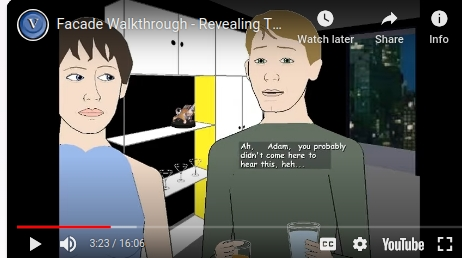
\includegraphics[width=0.8\textwidth]{facade.jpeg}

        NPCs are there to guide the player and are the projection of the game designers into the game world. 

        Because of this, is is really important that npcs have fluid dialogue and dont break the illusion of choice too easily.
        Current solutions imply using dialogue trees.
        Dialogue trees are an really good solution but they can still feel rough on the edges. and the illusion can be broken easily when u have to decide from a set of predefined dialogue choices.

        The imersiveness of games could greatly improve if ml were to be implemented on top of this already existing dialogue tree solution.

        Such solutions have already been experimented with, in the following i will present the findings of 2 other papers that use machine learning to improve npc dialogue and interaction.



        % \begin{figure}
        %   \begin{center}
        %     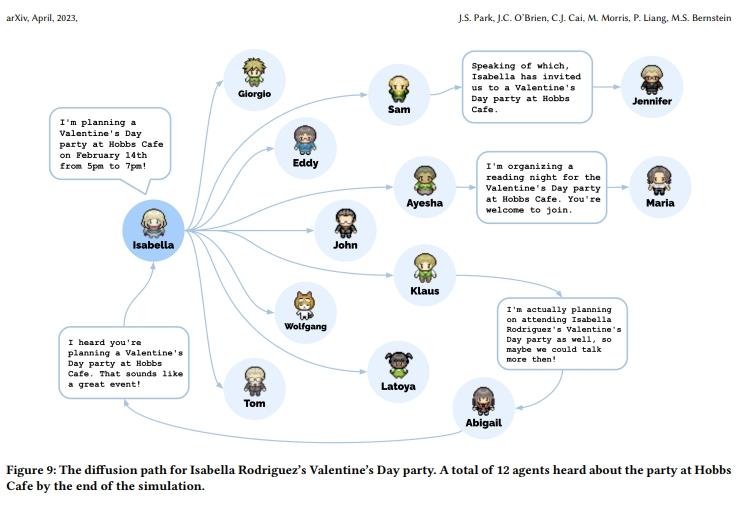
\includegraphics[width=0.8\textwidth]{birthdayParty.jpeg}
        %   \caption{Arch}
        %   \end{center}
        % \end{figure}

      \section*{Simulating Human Interaction}

        "Inworld Origins is a technical demo developed to demonstrate the power of generative AI-powered NPCs in video games. It showcases advanced NPC behavior and dialogue driven by artificial intelligence, leading to more immersive and personalized gaming experiences. The demo is set in a neo-noir sci-fi crime scene in the aftermath of an explosion in the city of Metropolis." source:google

          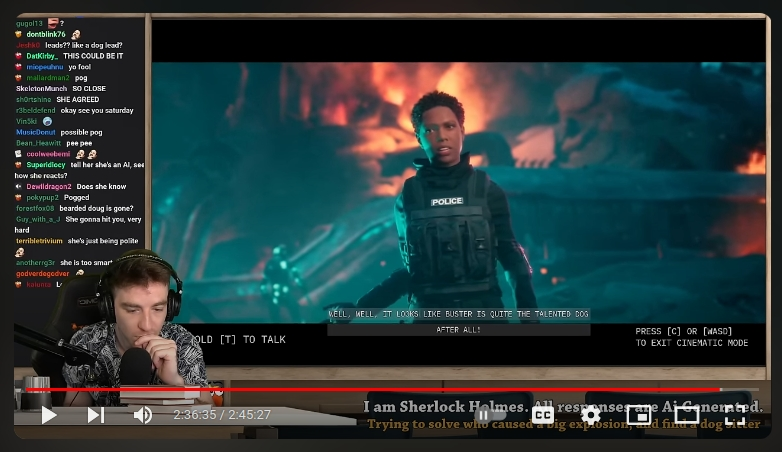
\includegraphics[width=0.8\textwidth]{dougdoug.jpeg}
          Screenshots of one demo using their openai abstraction layer.
          
        This team even offers multiple solutions for implementing such agents in popular environments such as Unreal.

        \textbf{Something that this project and the following one have in common is the presence of microphone input for live dialogue.}

          There is also a mod for the popular game Skyrim that allows the player to have fluid dialogue with any in-game character. 

        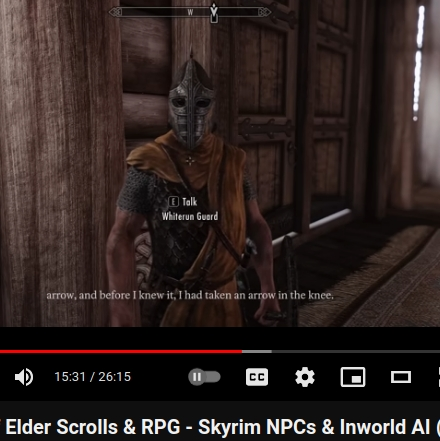
\includegraphics[width=0.8\textwidth]{arrow.jpeg}



          \subsection*{Ai interacting to Ai}
              One paper that i found beyond fascinating was Interactive Simulacra of Human Behavior.
        
              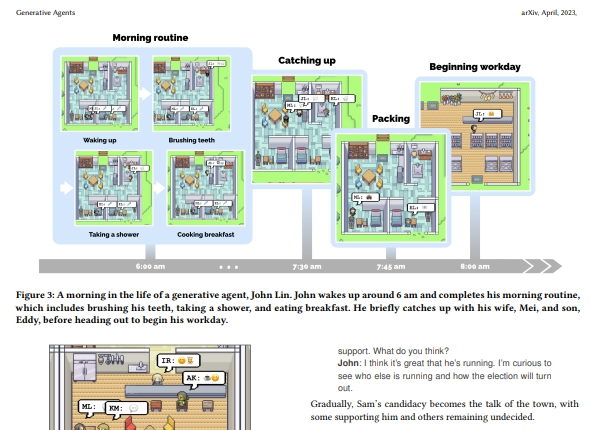
\includegraphics[width=0.4\textwidth]{morningRoutine.jpeg}
            
            They created an environment that allowed ml agents to communicate to one another. One of the most exciting outcomes was that one agent organised a birthday party and proceeded to invite other ml agents to the party. 

            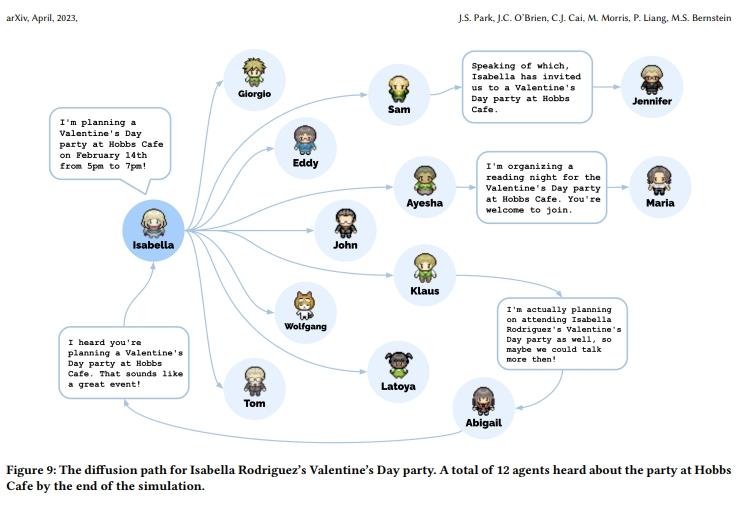
\includegraphics[width=0.8\textwidth]{birthdayParty.jpeg}

            The following goes more in detail over the implementatation design for one agent:
            
            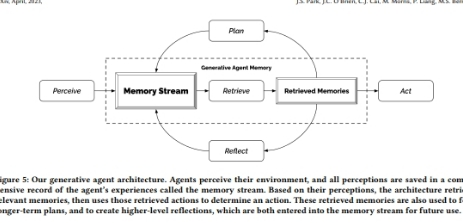
\includegraphics[width=0.8\textwidth]{DataStructure.jpeg}
            
            This design grants access to managing memories by long-time storage of relevant info. 

      
      \section*{Out-performing Human Performance}
        %   TODO: IMAGE 
        %   popular youtuber Code Bullet has a series where he "solves" games using AI models. He usually uses neural-networks for his solutions. 
          
          There are chess bots being developed that use machine learning in an attempt to "solve" the game of chess. So it is clear to say there is is a lot of incentivise towards acomodating machine learning algorithms into games.

        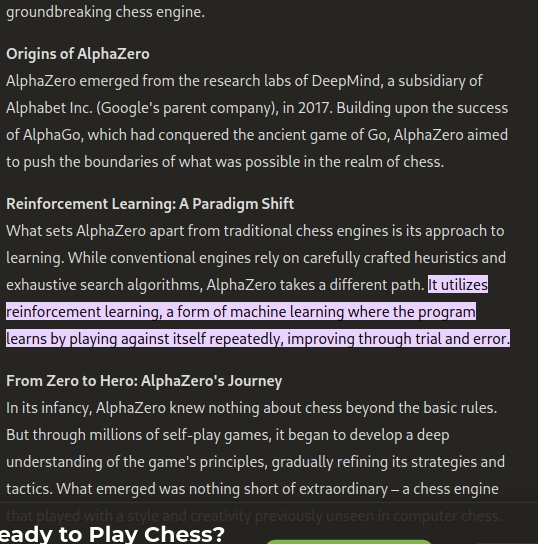
\includegraphics[width=0.8\textwidth]{alphazero.jpeg}







    % 



\part{Field Study}
% \addcontentsline{toc}{part}{Field Study}


  



\chapter*{Field Study - Introduction}
\addcontentsline{toc}{chapter}{Introduction}
  The Field Study chapters will present a brief explication of the moving parts that are involved in computer graphics rendering.

  First chapter is the one with more focus on embedded-systems concepts 
  Second chapter goes through graphics abstraction layers 
  Third chapter presents an overview of the popular solutions offered to end-users. 

%TODO WRITE
  \section*{Real-World use cases}
  % \addcontentsline{toc}{section}{use-cases}
      \subsection*{Student Projects - Stanford CS148 Computer Graphics and Imaging Course}
        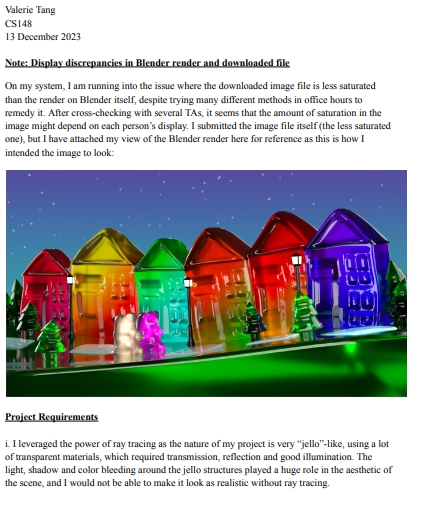
\includegraphics[width=0.5\textwidth]{stanford_softbodies.jpeg}

        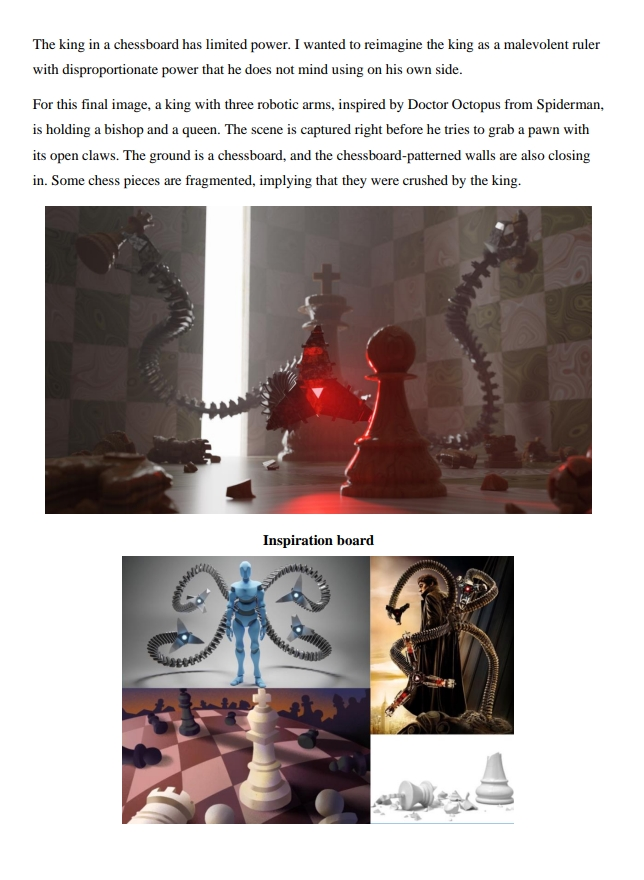
\includegraphics[width=0.5\textwidth]{stanford_chess.jpeg}


        % TODO TODO
      % \subsection*{Academic Research}
      %     IMAGES


  


\chapter*{Field Study - Hardware}
\addcontentsline{toc}{chapter}{Hardware}
  This chapter brings focus towards embedded systems by being a brief description of the process of getting the LEDs on our screens to display whatever the computer's video board decides to render. 
  \section*{The connection between screen and motherboard}
  % \addcontentsline{toc}{section}{Video cards}
    \subsection*{Proof of concept using Arduino}
      TINKERCAD IMAGE
        % \href{https://www.youtube.com/watch?v=l7rce6IQDWs}{video}
    \subsection*{Proof of concept using embedded circuits}
      BEN EATER VIDEO
    \subsection*{videoboards}
      LINUS TECH TIPS OLD VIDEO MANUFATEURS PCBs


  

\chapter*{Field Study - Software}
\addcontentsline{toc}{chapter}{Software}
  This chapter accepts the embedded solutions as they are and develops solutions that step forward. 
  The usual philosophy is developing abstraction layers.

    \section*{OPENGL - Motivation}
    % \addcontentsline{toc}{section}{opengl}
        There are a few options when choosing a graphics abstraction solution. The most popular in the game development industry are Vulkan and DirectX. DirectX is more appropriate when it comes to Windows-specific optimizations, while Vulkan profits from Low-level control and performance and performs better at High-performance applications with multi-threading.

        The only disadvantage to both those solution is that neither of them is as documented as opengl. Also, opengl is more popular in the educational/academic space and felt like the more appropriate choice.

    \section*{OPENGL - Features}
        OpenGL's extensive documentation comes with both positives and negatives. Being one of the oldest solution to this problem it had seen multiple refactoring stages throught the years, this is best observed when realising there is a new revision of the opengl superbible released every couple of years. Each presenting the usual "How-to" projects and also acting as an update journal.

        \pagebreak

        In the following i will briefly talk about popular opengl features.


  
        \subsection*{PHIGS Standard Compliant}
            Offers primitive support and for their attributes by using Rendering Algorithms that use the low-level per pixel drawing functions extensively.









    % \part{Implementation}
% \addcontentsline{toc}{part}{Implementation}




  
\chapter*{Mathematical Framework}


  


\part*{Implementation - Architecture}
\addcontentsline{toc}{chapter}{Architecture}

  \begin{center}
    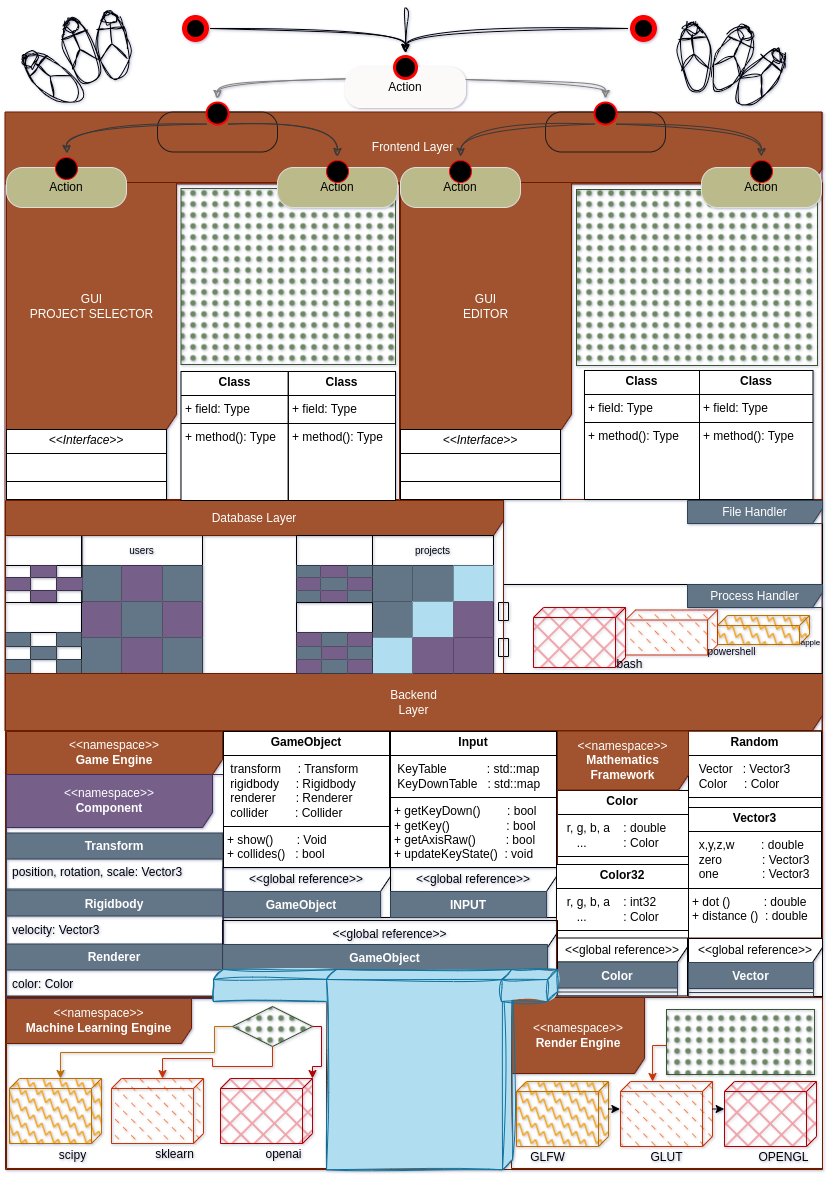
\includegraphics[width=\textwidth]{implementation_arch.png}
  \end{center}
  \pagebreak

  I intent for this project to become a collection of technologies that can be interconnected.
Similar to how Internet-of-Things solutions involve different running parts for achieving one goal, 
as such i want my software making environment to be as versatile as possible. 

  One obvious start impediment is going past the first couple of hello-world projects
  until you find a tool that does the job.

  The percentage of availability of one component can be determined by the color of one's title. 

    \textcolor {red} {bright  colors} means more relevant to this  \textcolor {orange} {iteration}.

    \textcolor {brown} {neutral colors} suggests the component's state of integrity and integration.

    \textcolor {gray} {non-colors} and you're looking at a component that hasn't been integrated yet.

  Future expansion possibilities are in \textcolor {white} {white} color. 


  \begin{itemize}
    \item  \textcolor {brown} { \textbf { FrontEnd ( PyQt   GUI programming interface)} } \\
    \textcolor {gray}   { integration dispatch layer  }
    \item \textcolor {red}    { Backend  ( Python Machine Learning Interface) } \\
      \textcolor {gray}   { communication socket }
    \item \textcolor {orange} { \textbf { Backend  ( C/C++  Render Engine,Math Engine) } }

    \textcolor {white}  { ROBOTICS / ARDUINO / PIE integration }
    % \item \textcolor {gray}   { FrontEnd ( web app ) }
    % \hline \textcolor {gray}   { integration dispatch layer  }
    % \item \textcolor {brown}  { Backend  ( Python Django ) }
    % \item \textcolor {gray}   { Database ( MariaDB) }
\end{itemize}



\pagebreak



\part*{The backend}

  There are two main languages used in this backend implementation:

  % \hline
  % \hspace{10}

  in C/C++  we have: Rendering Engine, Vectorial MathEngine, GameEngine.

  in Python we have: pyqt editor, Bash File Manager, Machine Learning Interface, Django.

  \chapter*{The Vectorial Math Engine}
  
\section*{Mathematical Framework with Homogenous Representation Support}

Intuitively, for storing a 3D point one might think about using a vector of length 3 ( maybe call them x, y, z ) and have a great day.
Well, this datastructure is good \emph{enough} for most cases.
There is, of course, one little edge-case in one of those cases where we might be needing a fancier solution.
Also, this fancy solution somewhat simplifies the other calculations as well.


This new datastructure implies using a k+1 dimentional vector space for representing k dimensional entities. 

% TODO:  REFERENCE HERE
Meaning that, in our application's purposes, a Vector3 class should store 4 elements. [More about this in future work]


% #include <iostream>
    % // Constructor with default parameters
% // C++ class definition for Vector2
\begin{lstlisting}
class Vector3 
{
  public:
    double x, y, z, w;
    Vector3(double _x, double _y = 0, double _z = 0, double _w = 1) 
           : x(_x), y(_y), z(_z), w(_w) { }
};
\end{lstlisting}


\begin{equation*}
    \mathbf{v_1} = \begin{pmatrix} x_1 & y_1 & z_1 & w_1 \end{pmatrix}.
\end{equation*}

\begin{equation*}
    \mathbf{v_2} = \begin{pmatrix} x_2 & y_2 & z_2 & w_2 \end{pmatrix}.
\end{equation*}





% int main() {
%     // Example usage of Vector3 class
%     Vector3 v1(1.0, 2.0, 3.0);
%     Vector3 v2(4.0, 5.0);

%     std::cout << "v1: (" << v1.getX() << ", " << v1.getY() << ", " << v1.getZ() << ", " << v1.getW() << ")" << std::endl;
%     std::cout << "v2: (" << v2.getX() << ", " << v2.getY() << ", " << v2.getZ() << ", " << v2.getW() << ")" << std::endl;

%     return 0;
% }


% we must be able to do with this DataStructure that would benefit of storing a 3D point as a 4D Vector (x, y, z, \textbf{\emph{w}}).


% This mathematical framework is very important because it assures that the phigs requirements can be fulfiled and how.


\pagebreak

\section*{Please do not be afraid of the \emph{w}.}

  \begin{equation}
    \emph{v.w} =
    \[ \begin{cases} 
      1 & ,\text{if v is used for describing a \hspace{8} point in space}\\ 
      % v ==Vector3::Point\\
      0 & ,\text{if v is used for describing an arrow in space} 
          % ,x::TYPE==Vector3::Arrow
       \end{cases}
    \]
    \label{}
  \end{equation}



Since \emph{w} is defined by a pretty straight-forward formula and the vector \textbf{usually} behaves like a point:


\begin{lstlisting}
    Vector3 v = new Vector3::one * 7
    Debug::Log(v); // <7,7,7,1>
\end{lstlisting}





% TODO: MATH FORMULA FOR w = 1, if point w = 0, if arrow

\section*{Data Structures}
\textbf{Vector Multiplication:}

\begin{equation}
    \mathbf{v_1} \cdot \mathbf{v_2} = (x_1 x_2) + (y_1 y_2) + (z_1 z_2) + (w_1 w_2)
\end{equation}

\textbf{Dot Product of Vectors:}

The dot product \( \mathbf{v}_1 \cdot \mathbf{v}_2 \) between vectors \( \mathbf{v}_1 \) and \( \mathbf{v}_2 \) is calculated as:

\[
\mathbf{v}_1 \cdot \mathbf{v}_2 = v_{1,1} \cdot v_{2,1} + v_{1,2} \cdot v_{2,2} + \cdots + v_{1,m} \cdot v_{2,m}
\]


\textbf{Constructing a Matrix from Vectors:}

Let \( \mathbf{v}_1 = (v_{1,1}, v_{1,2}, \ldots, v_{1,m}) \) be a vector representing the row elements.

Let \( \mathbf{v}_2 = (v_{2,1}, v_{2,2}, \ldots, v_{2,n}) \) be a vector representing the column elements.


\begin{lstlisting}
  v1 = Random::Vector3();
  v2 = Random::Vector3();
\end{lstlisting}


  % matrix = line.dot(column);

  % return matrix;



The resulting matrix \( \mathbf{M} \) formed by these vectors is:

\[
\mathbf{M} = \begin{pmatrix}
v_{1,1} & v_{1,2} & \cdots & v_{1,m} \\
v_{2,1} & v_{2,2} & \cdots & v_{2,m} \\
\end{pmatrix}
\]



  % \subsection*{Matrix Multiplication}
  % \begin{equation}
  %     \mathbf{A} = \begin{pmatrix}
  %     a_{11} & a_{12} & a_{13} & a_{14} \\
  %     a_{21} & a_{22} & a_{23} & a_{24} \\
  %     a_{31} & a_{32} & a_{33} & a_{34} \\
  %     a_{41} & a_{42} & a_{43} & a_{44}
  %     \end{pmatrix}
  % \end{equation}

  % \begin{equation}
  %     \mathbf{B} = \begin{pmatrix}
  %     b_{11} & b_{12} & b_{13} & b_{14} \\
  %     b_{21} & b_{22} & b_{23} & b_{24} \\
  %     b_{31} & b_{32} & b_{33} & b_{34} \\
  %     b_{41} & b_{42} & b_{43} & b_{44}
  %     \end{pmatrix}
  % \end{equation}

  % \begin{equation}
  %     \mathbf{C} = \mathbf{A} \times \mathbf{B} = \begin{pmatrix}
  %     c_{11} & c_{12} & c_{13} & c_{14} \\
  %     c_{21} & c_{22} & c_{23} & c_{24} \\
  %     c_{31} & c_{32} & c_{33} & c_{34} \\
  %     c_{41} & c_{42} & c_{43} & c_{44}
  %     \end{pmatrix}
  % \end{equation}


\pagebreak



\textbf{Matrix Multiplication (Traditional):}
\begin{equation}
    C = A \times B \quad \text{where} \quad C_{ij} = \sum_{k=1}^{n} A_{ik} \cdot B_{kj}
\end{equation}

% \begin{equation*}
%     c_{ij} = \sum_{k=0}^{4} v_{ik} v_{kj} = v_{i1}v_{1j} + v_{i2}v_{2j} + v_{i3}v_{3j} + v_{i4}v_{4j}
% \end{equation*}


\textbf{Strassen Matrix Multiplication (Recursive):}
\begin{equation}
    \mathbf{M}_1 = (A_{11} + A_{22})(B_{11} + B_{22})
\end{equation}
\begin{equation}
    \mathbf{M}_2 = (A_{21} + A_{22})B_{11}
\end{equation}
\begin{equation}
    \mathbf{M}_3 = A_{11}(B_{12} - B_{22})
\end{equation}
\begin{equation}
    \mathbf{M}_4 = A_{22}(B_{21} - B_{11})
\end{equation}
\begin{equation}
    \mathbf{M}_5 = (A_{11} + A_{12})B_{22}
\end{equation}
\begin{equation}
    \mathbf{M}_6 = (A_{21} - A_{11})(B_{11} + B_{12})
\end{equation}
\begin{equation}
    \mathbf{M}_7 = (A_{12} - A_{22})(B_{21} + B_{22})
\end{equation}


\section*{Software Engineering}

There are two main coordinate systems:

\textbf{Cartesian Coordinates:}
\begin{equation}
    (x, y, z)
\end{equation}

\textbf{Polar Coordinates:}
\begin{equation}
    (r, \theta, \phi)
\end{equation}

\textbf{Transformation Formulas:}
\begin{align}
    r &= \sqrt{x^2 + y^2 + z^2} \\
    \theta &= \arctan\left(\frac{y}{x}\right) \\
    \phi &= \arccos\left(\frac{z}{r}\right)
\end{align}







% LATE TODO 
% \begin{itemize}
%   \item Cartesian Coordinates
%   \item Polar     Coordinates 
% \end{itemize}

% Formulas for converting from one to another:
% \begin{itemize}
%   \item from Polar     to Cartesian
%   \begin{itemize}
%     \item cos(x)
%     \item sin(x)
%   \end{itemize}
%   \item from Cartesian to Polar
%   \begin{itemize}
%     \item x
%     \item y
%   \end{itemize}
% \end{itemize}


\pagebreak

In the following, we will take a look over the possible operation that are extensively used:

\textbf{Operations in Computer Graphics}

\textbf{Translation:}
\begin{equation}
    T(x, y, z) = \begin{pmatrix}
    1 & 0 & 0 & x \\
    0 & 1 & 0 & y \\
    0 & 0 & 1 & z \\
    0 & 0 & 0 & 1
    \end{pmatrix}
\end{equation}

\textbf{Scaling:}
\begin{equation}
    S(s_x, s_y, s_z) = \begin{pmatrix}
    s_x & 0 & 0 & 0 \\
    0 & s_y & 0 & 0 \\
    0 & 0 & s_z & 0 \\
    0 & 0 & 0 & 1
    \end{pmatrix}
\end{equation}



These equasions must be really easy to use. 
For this i have chosen the option that highly resembles Unity's ecosystem.


\begin{lstlisting}
void start();
void update();
int main() { Awake(); }
void Awake() {
  RenderEngine::setStart(start);
  RenderEngine::setUpdate(update);
  RenderEngine::setFixedUpdate(fixedUpdate);
  // MUST BE CALLED LAST
  RenderEngine::START(true);
}
void start() {
  Gameobject go; int speed = 0.01;
  Debug::Log(go.transform.name)
  Debug::Log(go.transform.position)
  
  go.transform.translate(Vector3::Right * speed)
  Debug::Log(go.transform.position)
  go.transform.position = Vector3::one * Math::sqrt(Math::pi);
  Debug::Log(go.transform.position)
}
\end{lstlisting}

The implementation feels self-explanatory from here. But for reference i advise 
\href{https://www.github.com}{source-code}





\pagebreak


Here lives the little inconvenience i mentioned at the beginning of the chapter 
that justified Homogenous Coordinates.

\textbf{Rotation with Euler Angles (XYZ order):}
\begin{equation}
    R_{XYZ}(\alpha, \beta, \gamma) = R_X(\alpha) \cdot R_Y(\beta) \cdot R_Z(\gamma)
\end{equation}
where
\begin{align}
    R_X(\alpha) &= \begin{pmatrix}
    1 & 0 & 0 & 0 \\
    0 & \cos\alpha & -\sin\alpha & 0 \\
    0 & \sin\alpha & \cos\alpha & 0 \\
    0 & 0 & 0 & 1
    \end{pmatrix}, \\
    R_Y(\beta) &= \begin{pmatrix}
    \cos\beta & 0 & \sin\beta & 0 \\
    0 & 1 & 0 & 0 \\
    -\sin\beta & 0 & \cos\beta & 0 \\
    0 & 0 & 0 & 1
    \end{pmatrix}, \\
    R_Z(\gamma) &= \begin{pmatrix}
    \cos\gamma & -\sin\gamma & 0 & 0 \\
    \sin\gamma & \cos\gamma & 0 & 0 \\
    0 & 0 & 1 & 0 \\
    0 & 0 & 0 & 1
    \end{pmatrix}
\end{align}

\textbf{Gimbal Lock Issue:} Euler angles suffer from gimbal lock, where two of the three rotational axes align, leading to a loss of one degree of freedom.

\textbf{Solution: Quaternions}
\begin{equation}
    q = \cos\left(\frac{\theta}{2}\right) + \sin\left(\frac{\theta}{2}\right)(u_x i + u_y j + u_z k)
\end{equation}
where \( \theta \) is the rotation angle and \( (u_x, u_y, u_z) \) is the unit vector representing the axis of rotation.




% In most of the cases, the equasions are really easy.

% \subsection*{Translation}
% \subsection*{Scalation}
% \subsection*{Rotation}
% \subsubsection*{Euler-Lock}
% And it would've been all so easy if it weren't for you! 

% Euler Lock is a problem that ocurs when we try to use euler coordinates in rotation aplications. This problem can become extremily dangerous when solving robotics solutions where you can't afford to ???

% \subsubsection*{Quaternions}
% For eliminating the euler-lock problem, quaternions are used. Quaternions are ??

% Formulas:









  \chapter*{The opengl Rendering Framework}
  
\section*{Color32}


\begin{lstlisting}
class color32
{
  public:
    unsigned int r, g, b, a;

    color32(double grayscale) 
           : color(grayscale, grayscale, grayscale, 1.0f) { }
    color32(double _r, double _g, double _b, double _a = 1.0f) {  }
};
\end{lstlisting}




As you can see, similar to the vector class, the color datastructure is also a 4D vector. This will come in handy when dealing with shaders. 


  \subsection*{Opposite Colors}
  \begin{lstlisting}
  class color32
  {
    public:
      unsigned int r, g, b, a;

      color32(double grayscale) 
             : color(grayscale, grayscale, grayscale, 1.0f) { }
      color32(double _r, double _g, double _b, double _a = 1.0f) {  }
  };



  \end{lstlisting}


  \begin{lstlisting}
  void start();
  void update();
  int main() { Awake(); }
  void Awake() {
    RenderEngine::setStart(start);
    RenderEngine::setUpdate(update);
    RenderEngine::setFixedUpdate(fixedUpdate);
    // MUST BE CALLED LAST
    RenderEngine::START(true);
  }
  void start() {
    Gameobject go;
    go.transform.position = Random::Vector3().normalised *  Random::Value(-5, 5); 
    Debug::Log(go.transform.position)
  }
  \end{lstlisting}


\section*{Primitives}

% PHIGS (Programmer's Hierarchical Interactive Graphics System) provides the function:

\begin{lstlisting}

  point(x, y, c); // Changes the color of the pixel at location <x, y> to c

  line(<<x>, <y>>, 
       <<x>, <y>>); // Draws a line between 2 points

  background(color);

  square(point1, point2);
  fill(color);
  circle(point , radius);

  noStroke();
\end{lstlisting}

% \begin{equation}
  % P(x, y), \forall x, y, -\frac{\text{screen::WIDTH}}{2} \leq x \leq \frac{\text{screen::WIDTH}}{2}
  % \label{eq:pixel}
% \end{equation}

These functions are the fundamental building blocks for rendering graphics on a screen in OpenGL. 
For the existance of these functions, 
OpenGL implements various procedures to draw shapes and perform graphical operations.

\subsection*{Points and Lines}

Points and lines are basic graphical primitives. A point is represented by its coordinates \((x, y)\) on the screen, and a line is represented by a linear equation.

\subsubsection*{Line-Drawing Procedure}

A line can be represented by the equation:

\begin{equation}
  y = mx + b
\end{equation}

where \( m \) is the slope of the line, calculated as:

\begin{equation}
  m = \frac{\Delta y}{\Delta x}
\end{equation}

% % ### DDA Algorithm (Digital Differential Analyzer)

% The DDA algorithm is an incremental method for drawing lines:

% \[
% \begin{align*}
%   \Delta x &= x_1 - x_0 \\
%   \Delta y &= y_1 - y_0 \\
%   \text{If } |\Delta x| > |\Delta y|, &\text{ then } \text{steps} = |\Delta x| \text{ else } \text{steps} = |\Delta y| \\
%   \Delta x_{\text{increment}} &= \frac{\Delta x}{\text{steps}} \\
%   \Delta y_{\text{increment}} &= \frac{\Delta y}{\text{steps}}
% \end{align*}
% \]

% Starting from \((x_0, y_0)\), the algorithm increments the coordinates:

% \[
% \begin{align*}
%   x &= x + \Delta x_{\text{increment}} \\
%   y &= y + \Delta y_{\text{increment}}
% \end{align*}
% \]

% % ### Bresenham's Line Drawing Algorithm

% Bresenham's algorithm uses integer arithmetic for efficient computation:

% \[
% \begin{align*}
%   \Delta x &= x_1 - x_0 \\
%   \Delta y &= y_1 - y_0 \\
%   \text{Decision parameter} \, p &= 2\Delta y - \Delta x
% \end{align*}
% \]

% For each \(x\) from \(x_0\) to \(x_1\):

% \[
% \begin{align*}
%   \text{If } p < 0, &\text{ then } p = p + 2\Delta y \\
%   \text{else}, &\text{ increment } y \text{ and } p = p + 2(\Delta y - \Delta x)
% \end{align*}
% \]

% % ### Line Attributes

% % #### Width

% Line width can be controlled using a parameter \(w\):

% \begin{equation}
%   \text{LineWidth}(w)
% \end{equation}

% % #### Color

% Color can be specified using RGB values:

% \begin{equation}
%   \text{Color}(r, g, b)
% \end{equation}

% % #### Segments

% A line segment between two points \((x_0, y_0)\) and \((x_1, y_1)\) can be drawn using the above algorithms, with the line attributes applied.

% \subsection*{Circle-generating Algorithms}

% % ### Midpoint Circle Algorithm

% The midpoint circle algorithm efficiently draws circles using the symmetry of circles and incremental calculations:

% \[
% \begin{align*}
%   x &= r, y = 0 \\
%   \text{Decision parameter} \, p &= 1 - r
% \end{align*}
% \]

% For each \(x\) from \(r\) to 0:

% \[
% \begin{align*}
%   \text{If } p < 0, &\text{ then } p = p + 2x + 3 \\
%   \text{else}, &\text{ decrement } y \text{ and } p = p + 2(x - y) + 5
% \end{align*}
% \]

% % ### Parametric Form

% Using the parametric form of a circle:

% \[
% \begin{align*}
%   x &= r \cos \theta \\
%   y &= r \sin \theta
% \end{align*}
% \]

% \subsection*{Flood-Fill Algorithms}

% Flood-fill algorithms fill a contiguous area of pixels with a specified color.

% % ### Boundary Fill Algorithm

% Starting from a seed point \((x, y)\):

% \[
% \begin{align*}
%   \text{If } P(x, y) \neq \text{boundary\_color} \text{ and } P(x, y) \neq \text{fill\_color}, &\text{ then fill } P(x, y) \text{ and apply to neighboring pixels}
% \end{align*}
% \]

% \subsection*{Text Renderer}

% Rendering text involves drawing each character glyph using the above primitives and positioning them appropriately.

% \section*{Conclusion}

% The described primitives and algorithms form the basis of graphical rendering in OpenGL, allowing the creation of complex images from basic elements like points, lines, and circles.













%       % \begin{itemize}
%       %   \item Points and Lines
%       %   \begin{itemize}
%       %     \item Width
%       %     \item Color
%       %     \begin{itemize}
%       %       \item Flood-Fill Algorithms
%       %     \end{itemize}
%       %     \item Segments
%       %   \end{itemize}
%       %   \item Circle-generating Algorithms
%       %   \item Text Renderer
%       % \end{itemize}

%   % \subsubsection*{Operations}
%   %   \begin{itemize}
%   %     \item Matrices
%   %     \begin{itemize}
%   %       \item Homogeneous Representation
%   %       \item Matrix      Multiplication
%   %     \end{itemize}

%   %     \item Basic Transformations
%   %     \begin{itemize}
%   %         \item Translation
%   %         % TODO: ADD EQUASIONS
%   %         \item Rotation
%   %         \begin{itemize}
%   %             \item Euler Method
%   %             \item Euler Problem
%   %             \item Quaternions
%   %             % TODO: EQUASIONS
%   %         \end{itemize}
%   %         \item Scaling
%   %         % TODO: EQUASIONS
%   %     \end{itemize}
%   %     \end{itemize}







% \section*{Game Engine Component}

% \subsection*{Render Engine}

% \begin{verbatim}
% namespace RenderEngine
% {
%     void Enabled(bool state);
 
%     void setStart (void (*func)());
 
%     void setUpdate(void (*func)());
% }
% \end{verbatim}

% The Render Engine namespace includes functions for enabling or disabling the engine, and setting start and update functions. These functions are represented as follows:

% \[
% \text{Enabled}(state) \rightarrow \text{void}
% \]

% \[
% \text{setStart}(\text{func}) \rightarrow \text{void}
% \]

% \[
% \text{setUpdate}(\text{func}) \rightarrow \text{void}
% \]

% Here, \(\text{func}\) is a function pointer that can be assigned to start or update functions for the engine.

% \subsection*{Vector3 Class}

% \begin{verbatim}
% class Vector3
% {
% public:
%   double x, y, z, w;
%   static Vector3 zero;
%   static Vector3 one;

%   Vector3() : Vector3(0, 0, 0, 1) {}
 
%   Vector3(double _x, double _y = 0.0f, double _z = 0.0f, double _w = 1.0f) 
%     : x(_x), y(_y), z(_z), w(_w) {}
 
%   Vector3& operator=(const Vector3& other);
%   Vector3& operator+=(const Vector3& other);
%   Vector3& operator*=(double scalar);
%   Vector3 operator*(double scalar) const;
%   Vector3 operator-(const Vector3& other) const; 
%   Vector3 operator+(const Vector3& other) const; 
%   double dot(const Vector3& other) const;
%   Vector3 operator/(double scalar) const;
% };
% \end{verbatim}

% Vector operations for the Vector3 class can be represented mathematically as follows:

% \[
% \mathbf{v} = \begin{pmatrix} x \\ y \\ z \\ w \end{pmatrix}
% \]

% Addition:
% \[
% \mathbf{v}_1 + \mathbf{v}_2 = \begin{pmatrix} x_1 \\ y_1 \\ z_1 \\ w_1 \end{pmatrix} + \begin{pmatrix} x_2 \\ y_2 \\ z_2 \\ w_2 \end{pmatrix} = \begin{pmatrix} x_1 + x_2 \\ y_1 + y_2 \\ z_1 + z_2 \\ w_1 + w_2 \end{pmatrix}
% \]

% Dot product:
% \[
% \mathbf{v}_1 \cdot \mathbf{v}_2 = x_1 x_2 + y_1 y_2 + z_1 z_2 + w_1 w_2
% \]

% Scalar multiplication:
% \[
% \mathbf{v} \cdot s = \begin{pmatrix} x \\ y \\ z \\ w \end{pmatrix} \cdot s = \begin{pmatrix} sx \\ sy \\ sz \\ sw \end{pmatrix}
% \]

% \subsection*{Color Class}

% \begin{verbatim}
% class Color
% {
% public:
%   float r, g, b, a;
%   /* 4bit color support */
%   static Color black;
%   static Color white;
%   static Color red;
%   static Color green;
%   static Color blue;
%   static Color yellow;
%   static Color cyan;
%   static Color magenta;
%   static Color gray;
%   static Color darkGray;
%   static Color lightGray;
%   static Color darkRed;
%   static Color darkGreen;
%   static Color darkBlue;
%   static Color brown;
%   static Color orange;
 
%   Color(double _value)
%     : Color(_value, _value, _value, 1.0f) {}
 
%   Color(double _r, double _g, double _b)
%     : Color(_r, _g, _b, 1.0f) {}
 
%   Color(double _r, double _g, double _b, double _a)
%     : r(_r), g(_g), b(_b), a(_a) {}
% };
% \end{verbatim}

% Colors in the Color class can be represented mathematically as:

% \[
% \mathbf{c} = \begin{pmatrix} r \\ g \\ b \\ a \end{pmatrix}
% \]

% Where \(r\), \(g\), \(b\), and \(a\) represent the red, green, blue, and alpha (transparency) components of the color, respectively.

% \subsection*{Component Namespace}

% \begin{verbatim}
% namespace Component
% {
%   class Transform
%   {
%     public:
%       Vector3 position; 
%       Vector3 rotation; 
%       Vector3 scale;    
%   };

%   class Rigidbody
%   {
%     public:
%       Vector3 velocity;
%   };

%   class Renderer
%   {
%     public:
%       Color color;
%   };
% }
% \end{verbatim}

% The Component namespace includes classes for Transform, Rigidbody, and Renderer components. Mathematically, these components can be represented as follows:

% \[
% \text{Transform} = \begin{pmatrix} \text{position} \\ \text{rotation} \\ \text{scale} \end{pmatrix}
% \]

% \[
% \text{Rigidbody} = \text{velocity}
% \]

% \[
% \text{Renderer} = \text{color}
% \]

% Where position, rotation, and scale are Vector3 objects, velocity is a Vector3 object, and color is a Color object.

% \subsection*{GameObject Class}

% \begin{verbatim}
% class GameObject
% {
% public:
%   Component::Transform transform;
%   Component::Rigidbody rigidbody;
%   Component::Renderer renderer;

%   GameObject();
% };
% \end{verbatim}

% A GameObject is composed of a Transform, Rigidbody, and Renderer component. This can be represented as:

% \[
% \text{GameObject} = \begin{pmatrix} \text{Transform} \\ \text{Rigidbody} \\ \text{Renderer} \end{pmatrix}
% \]

% Where each component is as defined in the Component namespace, representing the position, rotation, scale, velocity, and color of the GameObject.



  \chapter*{The Machine Learning libraries interface}
  \input{src/sections/mlInterface}

\part*{The Frontend}

  % This too, 
  % splits into two.

  % The software application and The web application.

  % As of writing this, no demonstrabable movement had been done in the web application department. 
  % The team lead suggests building software solutions that can be easily imported into web applications without needing to re-implement. Research had been done into webGL integration and the low-level graphics calls we use from opengl are compatible with webgl as well. 
  % There are even resources involving qt and pyqt integration. As of writing this, all of the GUI work had been done in the qt environment.  
  










    % \input{src/sections/webcrawler}
    







    % The software frontend is wrote in PyQt,a python wrapper for the industry standard qt.




\chapter*{pyroGamer - The PyQt Editor}

\section*{Introduction}
The frontend component is called "the PyroGamer project" and is organized into several directories and files. It includes functionalities for the Editor, Hub, and Splash interfaces. These components are managed through various Python scripts and stylesheets. The overall structure can be understood through the following.


\textbf{Directory Structure}

% The directory structure of the frontend is hierarchical. Let \( D \) represent the directory structure where:
\[
  \text{Directory } D := \{d_1, d_2, \ldots, d_n\}
\]
\[
  \text{typeOf} (\( d_i \)) \in \{\text{File}, \text{Directory}\}
\]
% can either be a file or a sub-directory containing further files or sub-directories.

\textbf{Components}

Most of the sub-modules start as this:
\[
F_m = S_m = \{\text{\_\_init\_\_.py}, \text{\_\_main\_\_.py}\}
\]

And then each of them comes with their own required technologies.


% \textbf{\emph{PROJECT LOADER}}

\[
  \text{let hub } H
\xrightarrow{\text{depend}}
\text{cli interface} 
\land 
\text{FileManager} 
\land 
(
\text{gui engine}
\land
\text{icons}
)
% \text{Tabs & Tables}
\]

% \textbf{\emph{Game Editor}}

\[
  \text{let editor } E 
\xrightarrow{\text{depend}}
\text{Hierarchy} 
\land 
\text{SceneView} 
\land 
\text{Inspector}
\land 
(
\text{Assets}
\land 
\text{Terminal}
)
\]

% \subsection*{Editor}
% The Editor component is represented by the set \( E \):
% \[
% E = \{e_1, e_2, \ldots, e_m\}
% \]
% where each \( e_i \) is a sub-directory or file under the Editor directory. Specifically:

\subsubsection*{Configs}
The Configs sub-directory contains scripts for configuration management:
\[
C = \{\text{FileManager.py}, \text{\_\_init\_\_.py}, \text{\_\_main\_\_.py}\}
\]

\begin{lstlisting}[language=Python, caption=FileManager.py]
import os

class FileManager:
    def __init__(self, path):
        self.path = path

    def list_files(self):
        return os.listdir(self.path)
\end{lstlisting}

\subsubsection*{Elements}
The Elements sub-directory is defined as:
\[
L = \{\text{Pages.py}, \text{Tabs}\}
\]
where Tabs itself is a set:
\[
T = \{\text{Assets.py}, \text{Hierarchy.py}, \text{Inspector.py}, \text{SceneView.py}, \text{Terminal.py}\}
\]

\begin{lstlisting}[language=Python, caption=Assets.py]
class AssetsTab:
    def __init__(self):
        self.assets = []

    def add_asset(self, asset):
        self.assets.append(asset)
\end{lstlisting}

\subsubsection*{FileManager and SceneManager}
Both FileManager and SceneManager sub-directories are represented as:
\[
F_m = S_m = \{\text{\_\_init\_\_.py}, \text{\_\_main\_\_.py}\}
\]

\begin{lstlisting}[language=Python, caption=__main__.py]
if __name__ == '__main__':
    print("Initializing Manager")
\end{lstlisting}

\subsubsection*{Styles}
The Styles sub-directory contains CSS files for styling:
\[
S_t = \{\text{createProjWindow.css}, \text{noProjectWindow.css}, \text{projectWindow.css}\}
\]

\subsection*{Hub}
The Hub component is represented by the set \( H \):
\[
H = \{ \text{Configs}, \text{Elements}, \text{icons}, \text{\_\_main\_\_.py} \}
\]

\subsubsection*{Configs}
The Configs sub-directory in Hub contains:
\[
C_h = \{ \text{FileManager.py}, \text{\_\_main\_\_.py} \}
\]

\subsubsection*{Elements}
The Elements sub-directory in Hub is:
\[
L_h = \{ \text{Tables.py}, \text{Tabs.py} \}
\]

\subsection*{Splash}
The Splash component contains:
\[
S_p = \{ \text{images}, \text{\_\_main\_\_.py} \}
\]

\section*{Inter-component Relationships}
The interactions between different components can be represented using functions and mappings. Let \( f: E \to H \) represent the function mapping elements from the Editor to the Hub. Similarly, \( g: H \to S_p \) represents the mapping from Hub to Splash.

\subsection*{File Management}
File management across different components is handled by the scripts in Configs and FileManager directories. Let \( \mathcal{F} \) be the set of file management scripts:
\[
\mathcal{F} = C \cup F_m \cup C_h
\]

\subsection*{Styling}
Styling is governed by CSS files in the Styles directory:
\[
\mathcal{S} = S_t
\]

The overall relationship between these parts can be expressed as:
\[
\text{Frontend} = \mathcal{F} \cup \mathcal{S} \cup (L \cup L_h) \cup S_p
\]

\section*{Conclusion}
The frontend component of PyroGamer is a well-structured combination of directories and files. Each part has a specific role, and their interactions can be mathematically represented to understand the flow and dependencies within the system.






    \pagebreak

  \chapter*{Implementation - Showcase}
\addcontentsline{toc}{chapter}{Showcase}













    % 
\part{Results}





  


\chapter*{Technical Review}
\addcontentsline{toc}{chapter}{Technical Review}


    In this chapter, we will inspect to what extent needs one piece of software to satisfy in order for it to be considered part of the collection containing game engine.
    
    \section*{Speed}
    % \addcontentsline{toc}{section}{Speed}
    \section*{Memory}
    % \addcontentsline{toc}{section}{Memory}

    \section*{DVD bouncer}
    % \addcontentsline{toc}{section}{DVD}
    \section*{Pong, The Game}
    % \addcontentsline{toc}{section}{Pong}

    \paragraph*{Wikipedia} "A game engine is a software framework primarily designed for the development of video games and generally includes relevant libraries
    % and support programs such as a level editor.
    (...).
    % Game engine can also refer to the development software supporting this framework, typically 
    % a suite of tools and features for developing games.
    The core functionality typically provided by a game engine may include a rendering engine ("renderer") for 2D or 3D graphics, a physics engine or collision detection (and collision response), sound, scripting, artificial intelligence, 
    (...)
    % networking, streaming, memory management, threading, localization support, scene graph, and video support for cinematics.
    "

    So, in order to satisfy this definition, a piece of software \emph{P} can be considered a game engine, if and only if \emph{P} satisfies the following:

    \begin{itemize}
        \item \emph{P} is a software framework
        \begin{itemize}
          \item {"A software framework is an abstraction in which software, providing generic functionality, can be selectively changed by additional user-written code. 
            (...) 
            It provides a standard way to build and deploy applications and is a universal, reusable software environment 
            (...)
            to facilitate the development of software applications, products and solutions. "} source: Wikipedia

            % \paragraph*{Wikipedia} {"A software framework is an abstraction in which software, providing generic functionality, can be selectively changed by additional user-written code.
            % % , thus providing application-specific software. 
            % (...)
            % It provides a standard way to build and deploy applications and is a universal, reusable software environment 
            % % that provides particular functionality as part of a larger software platform 
            % (...)
            % to facilitate the development of software applications, products and solutions. "}
            \begin{itemize}
                \item Generic functionality that can be selectively adapted based on user's code.
                \item provides a standard way of building and deploying applications
            \end{itemize}
        \end{itemize}
        \item \emph{P} includes a suite of relevant engines
    \end{itemize}






  







\chapter*{Future Improvements}
\addcontentsline{toc}{chapter}{Future Improvements}

In this chapter, we outline future directions for the project and discuss upcoming enhancements and integrations.

\section*{Packaged Builds}
\addcontentsline{toc}{section}{Packaged Builds}

The goal of this project is to eventually provide packaged builds for easier deployment and distribution. Specifically, we aim to package the project for AUR (Arch User Repository) and as a PyPi (Python Package Index) library.

Some progress has already been made towards this goal; an early build is available for installation using the following command:
\[
\text{pip install -i https://test.pypi.org/simple/ game-genie}
\]
Unfortunately, pip support had to be temporarily halted until the application reaches a more stable and mature state.

\section*{Performance Evaluation}
\addcontentsline{toc}{section}{Performance Evaluation}

In this section, we assess the performance aspects of the application, focusing on runtime efficiency and optimization opportunities.

\subsection*{Speed Analysis}
\addcontentsline{toc}{subsection}{Speed Analysis}

To evaluate the speed of the application, various benchmarks and profiling techniques were employed. Preliminary tests indicate that the application performs adequately for its current scope. However, further optimization is planned to enhance performance in areas where execution time is critical.

\subsection*{Optimization Strategies}
\addcontentsline{toc}{subsection}{Optimization Strategies}

Several strategies for optimization have been identified, including algorithmic improvements, caching mechanisms, and parallel processing utilization. These strategies aim to reduce computational overhead and improve overall responsiveness.

\section*{Conclusion}
\addcontentsline{toc}{section}{Conclusion}

The future improvements outlined here pave the way for a more robust and efficient application. By focusing on packaged builds and performance enhancements, we aim to provide users with a smoother and more optimized experience.











% \chapter*{Future Improvements}
% \addcontentsline{toc}{chapter}{Future Improvements}
%   This has been a journey and after reading this paper you should have a view through the window of progress. There are still many to implement and properly integrate. There will be multiple update journals of this type posted on the following.

% \section*{Packaged builds}
%   The scope of this project is to one day make it as an AUR package and also a PyPi library.

%   Some work has already been made in this direction in the matter that one of the early builds is available by running 'pip install -i https://test.pypi.org/simple/ game-genie' in any terminal.
%   Unfortunately, I had to interrupt pip support for until application grows into a more stable and mature form.

  % \input{src/chapters/results/}



    % \chapter{Bibliography} 
% \addcontentsline{toc}{chapter}{Bibliography}

\begin{itemize}
    \item Author1, \textit{Book1}, 2018
    \item Author2, \textit{Boook2}, 2017
\end{itemize}


    % % \addcontentsline{toc}{Part}{Overview}
  \chapter*{Introduction} 
  \addcontentsline{toc}{chapter}{Introduction5}

    In the following i will present to you my work of the past year. Work where i attempt to combine multiple computer sciences. 

  \chapter{Motivation}

      I chose this thesis project because of the extended knowledge i obtained during my computer science bachelors in the fields of computer graphics and machine learning and because of my personal interest in the field of game development.

      My goal was to apply some of those newly aquired concepts in a project that would benefit my long-term game development research. 

      The way i've decided to apply these concepts is by building a graphics framework compatible with some of the simpler machine learning solutions.

  \chapter{Goals}

      The goal is to build a game engine that has machine learning solutions already integrated. 
      In the following i will present the benefits of this goal.

      \section{Benefits of building your own game engine}
          \subsection{Standard industry practice}
              it is common for big companies to build their own in-house game engines and then develop their games on it.
              advantages:     provides competitive edge, security, integrity ...
              disadvantages:  cost, team special for that.

              it is common for smaller sized companies to develop their games/projects on already existing game engines  
              advantages:     already existing reources and docs, community, 
              disadvantages:  dificult to come up with unique style.

              On the following, i want us to analyse some of the game engines that there are. and draw out relevant particularities of each of them.

              for this i have chosen 1 Open Source graphics framework (p5.js), 1 closed software game engine (RAGE) and 1 restricted game engine (UNITY).

              \subsubsection*{RAGE}
                  even though this is a closed project and unaccesible to the public, over the years different screenshots and code snippets had been leaked and/or reverse-engineered and i would like us to take a look at some of the more expressive ones.
              \subsubsection*{Unity}
                  Even though unity's source code is not accesible to the public, the engine is completly free to use for any individual*.
              \subsubsection*{P5.js}
                  This graphics engine is completly free and \href[]{github.com}{open-source}

          \subsection{Educational purposes}
              i strongly believe that building a game engine had massively improved my abilities.

      \section{Benefits of integrating machine learning with gaming}

          ml is the new and fancy cool shiny thing that shows promising numbers and gets ppl hyped and everyone loves it and it must be implemented into everything that exists.

          game development is no exception.

          \subsection{Simulating Human Interaction}
              NPCs are important in games.

              NPCs are there to guide the player and are the projection the game designers into the game world. 

              Because of this, is is really important that npcs have fluid dialogue and dont break the illusion of choice too easily.

              Current solutions imply using dialogue trees.
              
              they can still feel rough on the edges. and the illusion can be broken easily when u have to decide from a set of predefined dialogue choices.

              the imersiveness of games could greatly improve if ml were to be implemented on top of this already existing dialogue tree solution.

              Such solutions have already been experimented with, in the following i will present the findings of 3 other papers that use machine learning to improve npc dialogue and interaction.
              Two of the following are solutions for human-to-ai dialogue and one of them simulates ai-to-ai.
              \subsubsection*{Ai interacting to Ai}
                  % TODO: Refactor and fact-check with paper.
                  One paper that i found extremily fascinating was \href[]{google.com}{TITLE} by AUTHOR. They created an environment that allowed ml agents to communicate to one another. One of the most exciting outcomes was that one agent organised a birthday party and proceeded to invite other ml agents to the party. In the following i will briefly go over the implementatation design for one agent:
                  
                  % there were cool images of tables for the datastructures used. they had a timetable and there was a complex way for managing memories and long-time storage of relevant info. 

              \subsection*{Ai interacting to humans}
                  Another paper that highlights machine-learning agents interacting in human-like behaviour is \href[]{google.com}{TITLE} by AUTHOR. This team even offers multiple solutions for implementing such agents in popular environments such as Unity or ??.

                  One popular demo of their plugin? is the game \href[]{google.com}{GAMENAME}. 
                  Game that illustrates a scenario where the player is a detective and has to figure out a case, with the added twist that comunicating with any of the non-playable-characters (NPCs) is made through the microphone and with openai dialogue. 
                  
                  There is also a mod for the popular game Skyrim that allows the player to have fluid dialogue with any in-game character. 
          
          \subsection{Out-performing Human Performance}
              popular youtuber Code Bullet has a series where he "solves" games using AI models. He usually uses neural-networks for his solutions. One recent such video is where he programmed a JUMP KING ml.
              
              There are chess bots being developed that use machine learning in an attempt to "solve" the game of chess. So it is clear to say there is is a lot of incentivise towards acomodating machine learning algorithms into games.



\part*{Field Study}
\addcontentsline{toc}{part}{Field Study}

\chapter*{Field Study - Introduction}
\addcontentsline{toc}{chapter}{Introduction}
    The Field Study chapters will present a brief explication of the moving parts that are involved in computer graphics rendering.

    First chapter is the one with more focus on embedded-systems concepts 
    Second chapter goes through graphics abstraction layers 
    Third chapter presents an overview of the popular solutions offered to end-users. 


    \section*{Real-World use cases}
    \addcontentsline{toc}{section}{use-cases}
        \subsection*{Student Projects - Stanford Computer Graphics Course}
            LINK
        \subsection*{Academic Research}
            IMAGES


\chapter*{Field Study - Hardware}
\addcontentsline{toc}{chapter}{Hardware}

    This chapter brings focus towards embedded systems by being a brief description of the process of getting the LEDs on our screens to display whatever the computer's video board decides to render. 

    \section*{The connection between screen and motherboard}
    \addcontentsline{toc}{section}{Video cards}
        \subsection*{Proof of concept using Arduino}
            TINKERCAD IMAGE
            % \href{https://www.youtube.com/watch?v=l7rce6IQDWs}{video}
        \subsection*{Proof of concept using embedded circuits}
            BEN EATER VIDEO
        \subsection*{videoboards}
            LINUS TECH TIPS OLD VIDEO MANUFATEURS PCBs

    % \section{Graphics Abstraction Layers}

    %     \subsection{Providers}


    %         \subsubsection{opengl}


    %             % Besides this book series, there is, of course, more literature around it. It's fair to say that is an field studied intensively.

    %             % In the following i will go through some of the relevant literature and highlight diverse concepts that made it into the implementation. 
    %             % \begin{itemize}
    %             %   \item OpenGL superbible
    %             %       \begin{itemize}
    %             %         \item 
    %             %       \end{itemize}
    %             % \end{itemize}
    %             % Computer Graphics 2nd Edition (in C) by Donald Hearn
    %             % \item *Rodica baciu manual operare opengl
    %             %     \begin{itemize}
    %             %       \item 
    %             %     \end{itemize}
    %         \subsubsection{vulkan}
    %         \subsubsection{directx}

    %     \subsection{Pipelines}

    %     \subsection{Game Engines}

\chapter*{Field Study - Software}
\addcontentsline{toc}{chapter}{Software}
    This chapter accepts the embedded solutions as they are and develops solutions that step forward. 
    The usual philosophy is abstraction layers.

    \section*{OPENGL - Motivation}
    \addcontentsline{toc}{section}{opengl}
        There are a few options when choosing a graphics abstraction solution. The most popular in the game development industry are Vulkan and DirectX. DirectX is more appropriate when it comes to ... , while Vulkan profits from ... and performs better at ... .

        The only disadvantage to both those solution is that neither of them is as documented as opengl. Also, opengl is more popular in the educational/academic space and felt like the more appropriate choice.

    \section*{OPENGL - Features}
        OpenGL's extensive documentation comes with both positives and negatives. Being one of the oldest solution to this problem it had seen multiple refactoring stages throught the years, this is best observed when realising there is a new revision of the opengl superbible released every couple of years. Each presenting the usual "How-to" projects and also acting as an update journal.

        \pagebreak

        In the following i will briefly talk about popular opengl features.

        \subsection*{PHIGS Standard Compliant}
            Offers primitive support and for their attributes by using Rendering Algorithms that use the low-level per pixel drawing functions extensively.

            \subsubsection*{Primitives}
                \begin{itemize}
                  \item Points and Lines
                  \begin{itemize}
                    \item Width
                    \item Color
                    \begin{itemize}
                      \item Flood-Fill Algorithms
                    \end{itemize}
                    \item Segments
                  \end{itemize}
                  \item Circle-generating Algorithms
                  \item Text Renderer
                \end{itemize}

            \subsubsection*{Operations}
              \begin{itemize}
                \item Matrices
                \begin{itemize}
                  \item Homogeneous Representation
                  \item Matrix      Multiplication
                \end{itemize}

                \item Basic Transformations
                \begin{itemize}
                    \item Translation
                    % TODO: ADD EQUASIONS
                    \item Rotation
                    \begin{itemize}
                        \item Euler Method
                        \item Euler Problem
                        \item Quaternions
                        % TODO: EQUASIONS
                    \end{itemize}
                    \item Scaling
                    % TODO: EQUASIONS
                \end{itemize}
                \end{itemize}


    \section*{Other Graphics Abstraction Layers}
    \addcontentsline{toc}{section}{Other Graphics Abstraction Layers}
        \subsection*{Vulkan}
        \addcontentsline{toc}{subsection}{Vulkan}
        \subsection*{directX}
        \addcontentsline{toc}{subsection}{DirectX}




\chapter*{Field Study - Game Engines}
\addcontentsline{toc}{section}{Other Graphics Abstraction Layers}

\part{Implementation}
% \addcontentsline{toc}{part}{Implementation}

\chapter*{Implementation - Architecture}
\addcontentsline{toc}{chapter}{Architecture}

    In case you haven't read the previous chapter i advise glimsing over the chapters' titles at least once because it would give better context on where my project lives in the graphics lifecycle.

    My Application is a Graphics Abstraction Layer that imitates industry standards when it comes to procedures used for ease of learning.
    Besides being an easy-to-use beginner-friendly tool because of following industry standard solution in the c++ rendering backend engine. At it's core, this rendering engine is built on top of a vectorial mathematics engine.

    The novelty that this project brings to the computer graphics world is the presence of a python Machine Learning backend that acts as an abstraction layer for simplifying the communication with services (openai, ollama) or with powerful machine learning libraries (scipy, skilearn) 


    % TODO: DRAW>IO DRAWINGS FOR ALL OF THOSE
    \addcontentsline{toc}{section}{Backend}
    \section*{The C++    backend}
    \section*{The Python backend}

    \addcontentsline{toc}{section}{Frontend}
    \section*{The C++    frontend programming interface}
    \section*{The Python frontend programming interface}

\chapter*{Comparison between results}
\addcontentsline{toc}{chapter}{Result Comparison}
    \section*{DVD bouncer}
    \addcontentsline{toc}{section}{DVD}

    \section*{Pong, The Game}
    \addcontentsline{toc}{section}{Pong}

\chapter*{The Machine Learning Interface}
\addcontentsline{toc}{chapter}{Features}
    \section*{interface for communicating with openai}
    \addcontentsline{toc}{section}{openai, oLlama}
    \section*{interface for communicating with scipy}
    \addcontentsline{toc}{section}{SciPy, SkiLearn}
    \section*{tool for web crawling}
    \addcontentsline{toc}{section}{Data Crawling}

\chapter*{Technical Review}
\addcontentsline{toc}{chapter}{Technical Review}
    \section*{Speed}
    \addcontentsline{toc}{section}{Speed}
    \section*{Memory}
    \addcontentsline{toc}{section}{Memory}


\chapter{Technical Review}
    In this chapter, we will inspect to what extent needs one piece of software to satisfy in order for it to be considered part of the collection containing game engine.
    
    \paragraph*{Wikipedia} "A game engine is a software framework primarily designed for the development of video games and generally includes relevant libraries
    % and support programs such as a level editor.
    (...).
    % Game engine can also refer to the development software supporting this framework, typically 
    % a suite of tools and features for developing games.
    The core functionality typically provided by a game engine may include a rendering engine ("renderer") for 2D or 3D graphics, a physics engine or collision detection (and collision response), sound, scripting, artificial intelligence, 
    (...)
    % networking, streaming, memory management, threading, localization support, scene graph, and video support for cinematics.
    "

    So, in order to satisfy this definition, a piece of software \emph{P} can be considered a game engine, if and only if \emph{P} satisfies the following:

    \begin{itemize}
        \item \emph{P} is a software framework
        \begin{itemize}
          \item {"A software framework is an abstraction in which software, providing generic functionality, can be selectively changed by additional user-written code. 
            (...) 
            It provides a standard way to build and deploy applications and is a universal, reusable software environment 
            (...)
            to facilitate the development of software applications, products and solutions. "} source: Wikipedia

            % \paragraph*{Wikipedia} {"A software framework is an abstraction in which software, providing generic functionality, can be selectively changed by additional user-written code.
            % % , thus providing application-specific software. 
            % (...)
            % It provides a standard way to build and deploy applications and is a universal, reusable software environment 
            % % that provides particular functionality as part of a larger software platform 
            % (...)
            % to facilitate the development of software applications, products and solutions. "}
            \begin{itemize}
                \item Generic functionality that can be selectively adapted based on user's code.
                \item provides a standard way of building and deploying applications
            \end{itemize}
        \end{itemize}
        \item \emph{P} includes a suite of relevant engines
    \end{itemize}



\chapter{Conclusions}
    
    \section{Summary of this paper}
        This has been a journey and after reading this paper you should have a view through the window of progress. There are still many to implement and properly integrate. There will be multiple update journals of this type posted on the following.

    \section{Future improvements}
        

        \subsection{Packaged builds}
            The scope of this project is to one day make it as an AUR package and also a PyPi library.

            Some work has already been made in this direction in the matter that one of the early builds is available by running 'pip install -i https://test.pypi.org/simple/ game-genie' in any terminal.
            Unfortunately, I had to interrupt pip support for until application grows into a more stable and mature form.


        \subsection{}
            This project could just as well transform into an companion app for a 

        % \subsection{What is a game engine?}
        %     Maybe it feels irrelevant to talk about game engines when the project title says graphics engine, but in reality the graphics engine is one of the core components of a game engine. 
            
        %     A graphics engine is complex task in itself, besides the renderer itself, it requires a math backend and ways for fast inter-process communication.

        %     These being said, let's formally define a game engine!


        % \paragraph*{Paper} Providing frameworks for reusability and separation of concerns is key to software development today. 
        % % https://www.scirp.org/html/4-9301886_47999.htm



        % % \paragraph*{Axiom} A framework provides a collection of operations, data-structures and procedures and has specific "magic formulas" that allow the end-user to communicate with the base functionalities. 



        Licenses:

        \begin{itemize}
            \item Closed source with closed access
            \item Closed source with open access
            \item Open Source
        \end{itemize}

        Closed source game engines are usually a sign that the project is owned by a big company with a big number of employees and generous funding.
        
        It is unusual for a game company to provide access to its game engine to the end-users. This could be exploited into a competitive disadvantage.
        Although, once in a while, because of leaks or because of reverse-engineering some parts of the ecosystem are revealed to the public.

        In the following i will insert some snapshots of Rockstar's RAGE engine that had older versions reverse engineered and the newer ones leaked. 
        
        % images here

        As you can see, the environments offer statistics relevant to development.

        A closer inspection on figure [??] shows this line of code: "" that would indicate that ...


        % For the scope of this argument i will say that there are 2 main ways of developing a game and the choice is dependent on the size and budget of the developing team.

        The two options are either building an in-house framework 
        % around the subject and because i thought i could combine all of my past research into this.

        Before i even started writing, i already had experience working in the following fields and i will briefly present my computer science background



        \subsection{What should a game engine do?}
            In this subsection i will describe some of the tools that i would like my game engine to be able to offer.
            I will ilustrate this by showcasing some projects from my personal repertoir that had been built in a variety of environments and highlight the relevant tools that each environment offered me.
            % The following sections highlight pieces of my work that are relevant to this thesis. Each included project is significant due to specific implementations that are directly or indirectly connected to this paper.

            \subsubsection{Computer Graphics Experience}
                \begin{SCfigure}[0.9][h] 
                    \caption{Fractal Tree Visualization
                    
                    (usage of p5.js primitive functions in a recursive manner)

                    \href{https://www.youtube.com/watch?v=ajd0GGZgnDg&list=PL-j3UE1st04BZqRXq6eUBHpovhKjA1kiX&index=7}{showcase}}
                    
                    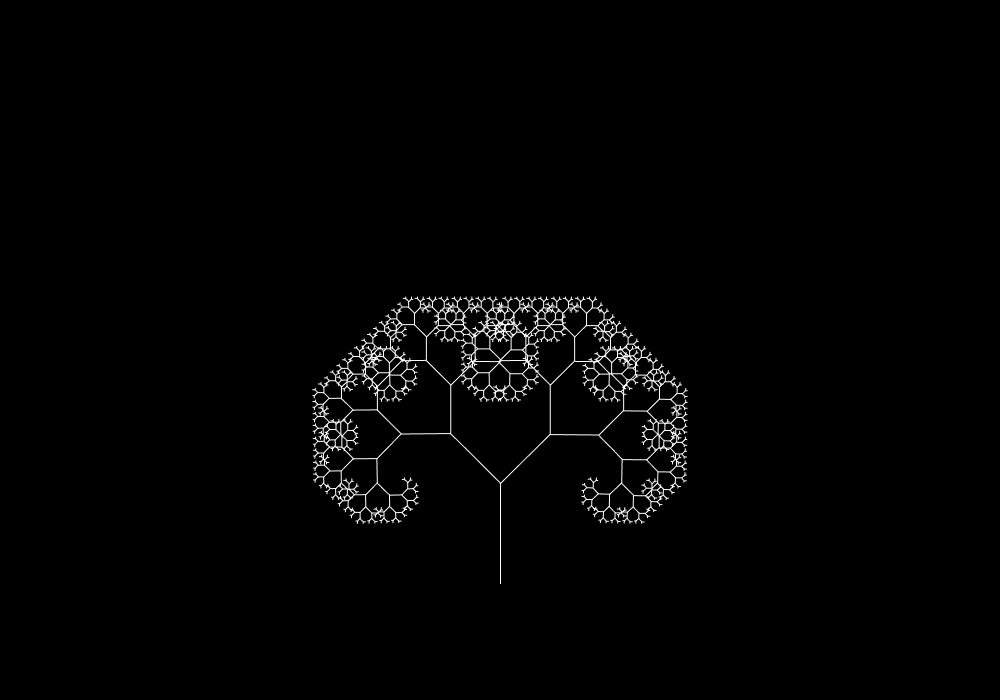
\includegraphics[width=8cm]{fractal.png}
                    \centering
                \end{SCfigure}                    
                \begin{itemize} 
                    \item Supershape Rendering Techniques 
                    \item Function Visualizer in OpenGL 
                    \item Complex Function Visualizer 
                \end{itemize}

            \subsubsection{Game Development Experience} 
                \begin{itemize} 
                    \item 3D Open World Environment Development 
                    \item Studies of Vector Movements in Unity 
                \end{itemize}

                % \subsubsection{in computer graphics}
            %     \subsubsection{fractal tree}
            %     \subsubsection{supershapes}
            %     \subsubsection{visualising basic function in opengl}
            %     \subsubsection{moving towards complex functions (mandelbrot series, julia fatou series)}
            %     \subsubsection{3D rendering}

            \subsubsection{in game development}
                my game development studies had mostly been around 3D open-world games. Being fascinated by rockstar's grand theft auto series i want to build something similar. i always wondered how cj was able to move in all the directions and calculating how there would be way too many paths to generate all the possible outcomes. so there should be smarter ways to do movement.
                And there is. Using vectors.
                My unity projects were mostly about perfectioning the 3D vector movement. Something that i also tried to implement in the opengl framework.   

        \subsection{Goal}
            I challenged myself to dig deeper into Game Development. I wanted to understand what makes all the pretty images move. i already had somewhat of an understanding of how the frames have to be processed independently and displayed in a fastly manner in order to trick the brain. but i wanted to go deeper then that.

            i already understood how to do certain simple tasks in unity, but i was so fascinated of the "transform.position = Vector2.One * scalar" command that i wanted to create a similar environment. 




            the intention of this project is to act as a foundation for a possible game engine that i will continue to deveop in the future. 

            a game engine is no easy task, there are many running parts and each of them must be SOLID. 

        % \subsection{Progress}

        %     until now i have the opengl framework in a stable state, this journey gave me a deeper understanding of all the running parts needed. 

        %     Now that i've been able to replicate some of the foundational concepts in enclosed environments, in the future i tend to use some already existing frameworks for physics and scene management and also ml libraries like scipy.

    \section{Literature Review}
        In this section i will explore other's solutions to the problem i was trying to solve.

        Unfortunately, there aren't many studies regarding "Machine Learning Compatible Game Engines" so i had to broaden my search.

        \subsection{Simulating Human Interaction}
                % TODO: Refactor and fact-check with paper.
            One paper that i found extremily fascinating was \href[]{google.com}{TITLE} by AUTHOR. They created an environment that allowed ml agents to communicate to one another. One of the most exciting outcomes was that one agent organised a birthday party and proceeded to invite other ml agents to the party. In the following i will briefly go over the implementatation design for one agent:
            
            % there were cool images of tables for the datastructures used. they had a timetable and there was a complex way for managing memories and long-time storage of relevant info. 

            Another paper that highlights machine-learning agents interacting in human-like behaviour is \href[]{google.com}{TITLE} by AUTHOR. This team even offers multiple solutions for implementing such agents in popular environments such as Unity or ??.

            One popular demo of their plugin? is the game \href[]{google.com}{GAMENAME}. 
            Game that illustrates a scenario where the player is a detective and has to figure out a case, with the added twist that comunicating with any of the non-playable-characters (NPCs) is made through the microphone and with openai dialogue. 
            
            There is also a mod for the popular game Skyrim that allows the player to have fluid dialogue with any in-game character. 
        
        \subsection{Out-performing Human Performance}
            popular youtuber Code Bullet has a series where he "solves" games using AI models. He usually uses neural-networks for his solutions. One recent such video is where he programmed a JUMP KING ml.
            
            There are chess bots being developed that use machine learning in an attempt to "solve" the game of chess. So it is clear to say there is is a lot of incentivise towards acomodating machine learning algorithms into games.

        \subsection{Bibliography Review}
            % this might be more relevant in an bibliography overview chapter
            in order to achieve this project i have went through multiple pieces of literature.

            the ones i used most extensively are:
                \subsection{Books}
                    \subsubsection{OpenGL SuperBible}
                        SuperBible provided a thorough introduction to OpenGL,
                        detailing its functions and capabilities. This resource
                        was instrumental in understanding the core principles of
                        rendering and shading, which are fundamental to the
                        development of any graphics application. By following
                        the examples and exercises in this book, I was able to
                        implement efficient rendering pipelines and gain a deep
                        understanding of shader programming.
                    \subsubsection{Computer Graphics (Donald Hearn)}
                        % this gave me an in-depth understanding of the computer graphics field and also very insightful insides to primitives, drawing algorithms, popular solutions to popular problems. 
                        Donald Hearn's Computer Graphics offered a comprehensive overview of graphics
                        primitives and the algorithms used to draw them. The book's clear explanations
                        of line drawing algorithms, polygon filling techniques, and transformations were
                        particularly beneficial. Implementing these algorithms in my application allowed
                        me to create accurate and efficient rendering routines.
                    \subsubsection{Mathematics for Game Development (Christopher Tremblay)}
                        % i held this book very closely while writing the math engine for the game-engine.
                        % i recaped my veVctorial knowledge and understood which operators are most relevant in such projects and why. 
                        Christopher Tremblay's book on
                        mathematics for game development provided a solid
                        foundation in vectorial math, which is crucial for tasks
                        such as collision detection and physics simulation. The
                        detailed explanations of vector operations, matrix
                        transformations, and geometric algorithms were directly
                        applied in the development of the vector math library in
                        my application.
                    \subsubsection{C++ (Bjarne Stroustrup)}
                        Bjarne Stroustrup's definitive
                        guide to C++ significantly improved my programming
                        skills, enabling me to write efficient, robust, and
                        maintainable code. The book's coverage of advanced C++
                        features, such as templates, polymorphism, and the
                        Standard Template Library (STL), was particularly
                        valuable in structuring my application and optimizing:want
                        performance.
                \subsection{Papers}
                    \subsubsection{ml agents that can communicate to one another}
                    \subsubsection{comp graphics projects from stanford}
                    \subsubsection{...}

    \section{from leds to opengl}
        \subsection{Why does my computer need a graphics card?}
            There is this extremily interesting video that showcases how easily one can communicate through the VGA protocol with any display. (BEN EATER)

            There are X many pins on a VGA port. From which, X1 are GROUND, X2 are VCC and 4? are used for actually displaying.

            The algorithm loop is fairly straight-forward: The monitor expects data through Y pin every Z miliseconds. Every piece of data is considered to be a pixel on the grid, if there is data sent through W pin, the monitor knows to skip to the next line.

            The setup revolves around telling the monitor the display resolution, refresh rate and bitmap? of the colors. 

            Roughly speaking, an led can receive anywhere from 0V to 3.3V (of course this can get more complicated depending on the color of the led). This is electronics-language but computer programs dont work with volts, they work with variables. A translation convention is needed.

            This 0V-3.3V range can be devided into however many steps but 255 steps is the most popular and widely accepted one. 
            Fun Fact: old apple/MSDOS/... computers are using 2Bit colors. That meaning that any led can be either completly turned on or off.

            Also old computers were using 1Led/Pixel and now we use 3LEDs/Pixel.
        \subsection{Colors and Vectors}
            So we need a data-structure that can hold 3 255bit values: r, g and b. Throw in an extra one for opacity and make it a vector.

            % image of color class

            This data-structure should be used repetedly and continuosuly because there are many pixels in a line and there are many lines in a display matrix.

            This color class is inherited from the vector class because it makes some calculations easier.

            % image of vector3 base class

            This Vector3 Class is the class that is used regulately

        \subsection{Computer Graphics}
        \subsection{Game Development}
        \subsection{Coding Practices}

    \section{from opengl to end-users}
        This is the space in the rendering pipeline that my project desires to occupies. 

% The first ever game created was 'Tennis for Two' and was played on an oscilloscope. From then, gaming evolved from simple pixelated experiences to complex, immersive digital worlds.

% "Before game engines, games were typically written as singular entities: a game for the Atari 2600, for example, had to be designed from the bottom up to make optimal use of the display hardware (...) 
% Even on more accommodating platforms, very little could be reused between games."

% (Game Engine, Wikipedia)

% % (Did u know that the first Roller Coaster Tycoon was written completly in Assembly?)

% Programmers needed a way to make the game building process more efficient. So around the mid-1990s, thanks to Epic Games and their launch of the Unreal Engine and thanks to Id Software's Doom and Quake games the term "Game Engine" started to become more and more popular.

% Fast forward mid-2020s, now we have access to ultra realistic tank simulators for soldier training ( projectName ), surreal worlds filled with fantasy creatures ( Middle Earth: Shadow Of Mordor ) and even indie projects like Hyerbolica that portraits how a non-euclidian world would behave like. Projects like these would've been way harder ( if not actually impossible ) to pull off without the help of game engines.

% \pagebreak

% \section{Game Engines}
% "The line between a game and its engine is often blurry. Some engines make a reasonably clear distinction, while others make almost no attempt to separate the two. ( ... ) We should probably reserve the term
% 'game engine' for software that is extensible and can be used as the foundation for many different games without major modification."

% ( Game Engine Architecture. by Jason Gregory )

% \begin{figure}[!h]
%     \centering
%     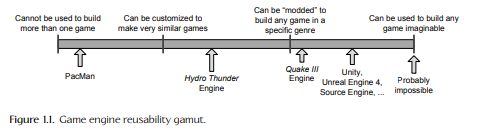
\includegraphics[width=1\linewidth]{chapters/gameEngine Usability.png}
%     \caption{Game Engine Reusability Gamut}
%     \label{fig:Game-Engine Reusability}
% \end{figure}



% Behind the curtains of any interactive application there is most likely a Game Engine. 
% You have probably heard before about Unity and Unreal but there are many more game engines out there. Some of them are In-House, some of them are Open-Source, some of them are made for a specific Genre. But none of them is offering Built-In Machine Learning Integration. 

% \subsection{What does a Game Engine offer?}

% While not limited to, some of the tools we expect a game engine to offer are: 
% \begin{enumerate}
%     \item Input Handling
%     \item Player Mechanics
%     \item Game-Specific Rendering
%     \item Collision \& Physics
%     \item Audio Playback
%     \item Game Cameras
%     \item Ai \& Behaviour Management
%     \item Online Multiplayer
%     \item Scene Graph
%     \item Scripting System
%     \item Visual Effects
% \end{enumerate}

% \section{What is Machine Learning?}

% \begin{enumerate}
%     \item predicts text, predicts what the next word in a sentence would most likely be.
%     \item it's too broad of a topic to be able to explain in detail in just one paper. And it's also not the purpose of this paper. This paper only wants to use the power of ai to simulate better npc's in games.
%     \item for the purpose of this, i will not try to recreate or train an machine learning model, i will use an already existing one: GPT 3.5-Turbo by OpenAI.
% \end{enumerate}

% \subsection{Machine Learning in Game Engines}
% \begin{enumerate}
%     \item Inworld Origins are already working on a solution for implementing GPT4 to be used in a NPC dialogue scenario.
%     \item There is this study where multiple GPT4 agents that can simulate believable human behavior. (Generative Agents: Interactive Simulacra of Human Behavior)
%     % https://arxiv.org/pdf/2304.03442.pdf
%     \item Currently, there are no game engines that have Machine Learning Systems built-in. 
% \end{enumerate}

% \section{Scope and Objectives of the Thesis}
% \begin{enumerate}
%     \item exploration, development, and evaluation of a game engine that integrates GPT-based machine learning capabilities 
%     \item explore the architecture of a game engine while building a basic one in Python using OpenGL.
%     \item explore what it means to add machine learning capabilities to a game engine. 
%     \item The focus of this research is on leveraging the power of natural language processing (NLP) and GPT models to enhance various aspects of game development, including storytelling, character interactions, procedural content generation, and player experiences.
% \end{enumerate}


    % % \chapter*{Motivation} 
\addcontentsline{toc}{chapter}{Motivation}
 
% \begin{enumerate}
%     \item Game engines provide the foundation for creating interactive digital experiences.
%     \item Machine Learning is a real Game Changer, promising a lot of advancements in almost every field.
%     \item For the past couple of years, the most advancements in the game development ecosystem were made in graphics.
%     \item Many significant breakthroughs had also been achieved in gameplay.
%     \item Not so many improvements on the Narrative.
%     \item Not anymore.
    
%     \item Transformers for Text Generation ( like ChatGPT ) can and will bring a huge innovation in the narrative component of games.
%     \item So there is a gap in the current game development ecosystem. A gap that sooner or later will be filled by the corporate giants. ( NVDA already working a lot on ai stuff... )
%     \item Although there are already many solutions on the market for artificial intelligence driven dialogue.
%     % ( Inworld Origins or https://arxiv.org/pdf/2304.03442.pdf )  ( Solutions which I'm going to use for inspiration as well) 
%     At the moment of publishing this, there is no comprehensive game engine that can seamlessly integrate machine learning capabilities.
%     \item My reasearch aims to design, develop, and evaluate a game engine that incorporates GPT-based machine learning capabilities. I want to demonstrate the feasibility and potential of this approach through the creation of practical game examples.
% \end{enumerate}



    % 
    % % \chapter{Computer Graphics}

    \section{Math Engine}
        \subsection{vector.cpp}
            the Vector3 class supports operations such as addition, subtraction, dot product, and cross product, enabling users to perform complex calculations with ease.
        \subsection{random.cpp}
            Generating true-randomness is one of the biggest computer science challenges. 

            In my project i needed a way the user to be able to get a "insert formal specs here for non-deterministic random" vector3 and color variable. 

            Lukily, i have stumbled upon this random-generator function and was able to implement it. Now, in the framework there is a function that returns a different each call random variable and also the seed is randomized so it differes between individual launches of the application. 
    \section{Renderer Engine}
        \subsection{primitives}
            OpenGL and WebGL are quite similar. P5.js is built on top of WebGL and offers the end-user (besides many more) a set of convenient functions for simple tasks like drawing the background, drawing a square, a circle, choosing stroke width and color.
        
            besides these functions i have thought of implementing classes for each of the base geometrical shapes. This implementation will come in handy when integrating with the game engine stuff (see chapter3:Game Development, section GameObjects). For example, each renderer component will use one of the primitive classes (square, circle, box, sphere) to display itself on the screen.
            
        \subsection{Transformations}
            As we've already mentioned in the mathematics chapter, transformations are a big deal when dealing with game development. They basically give fluidity. Also, they can be a tough challenge to overcome, especially because it requires the mathematical framework to be able to do complex calculations and as quickly as possible. 

            This topic is brought up multiple times in this paper and in this chapter we will focus on the specifics on how primitives transform.
            
            types of transformation:
            \begin{itemize}
                \item translation
                \item rotation
                \item scaling
                \item skewing
                \item warping
                \item ...
            \end{itemize}

            fun fact: did u know that u can achieve a rotation by doing multiple skew transformations in a row?
        \subsection{color.cpp}
    \section{Collision Detection}



% \section{Titlul secțiunii 1}

% \begin{figure}
%     \centering
%     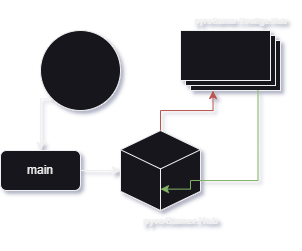
\includegraphics[width=0.5\linewidth]{chapters/pyroGamerHub.png}
%     \caption{Enter Caption}
%     \label{fig:enter-label}
% \end{figure}

% Id donec ultrices tincidunt arcu non sodales neque. Integer eget aliquet nibh praesent. Euismod in pellentesque massa placerat duis ultricies lacus sed. Mauris ultrices eros in cursus turpis massa. Integer quis auctor elit sed vulputate mi. Nibh ipsum consequat nisl vel pretium lectus quam id leo. Vel elit scelerisque mauris pellentesque pulvinar pellentesque. Suscipit tellus mauris a diam maecenas. Ultrices eros in cursus turpis massa tincidunt. Tristique senectus et netus et malesuada fames ac turpis egestas. Suspendisse interdum consectetur libero id faucibus nisl tincidunt eget. Sed risus pretium quam vulputate dignissim suspendisse in. Donec adipiscing tristique risus nec feugiat in fermentum posuere. A lacus vestibulum sed arcu non odio euismod lacinia at.

% \section{Titlul secțiunii 2}

% Pellentesque pulvinar pellentesque habitant morbi tristique senectus et. Ornare suspendisse sed nisi lacus sed viverra tellus in hac. Non sodales neque sodales ut etiam sit. In hendrerit gravida rutrum quisque non. Diam quam nulla porttitor massa id neque aliquam. Diam sit amet nisl suscipit adipiscing bibendum est ultricies integer. Cras fermentum odio eu feugiat pretium nibh ipsum. Egestas integer eget aliquet nibh praesent tristique magna. Porttitor eget dolor morbi non arcu risus quis varius quam. Gravida rutrum quisque non tellus orci. Diam volutpat commodo sed egestas egestas.
    % % \chapter{Game Development}
    \section{Game Engine}
        \subsection{GameObjects}
        \subsection{Components}
    \section{Collision Detection}
    % % \chapter{Machine Learning}
    \section{Probabilities}
    \section{Scipy compatibility}
    % 
    % % \chapter*{Concluzii} 
\addcontentsline{toc}{chapter}{Concluzii}

Lorem ipsum dolor sit amet, consectetur adipiscing elit, sed do eiusmod tempor incididunt ut labore et dolore magna aliqua. Nunc mattis enim ut tellus elementum sagittis vitae et. Placerat in egestas erat imperdiet sed euismod. Urna id volutpat lacus laoreet non curabitur gravida. Blandit turpis cursus in hac habitasse platea. Eget nunc lobortis mattis aliquam faucibus. Est pellentesque elit ullamcorper dignissim cras tincidunt lobortis feugiat. Viverra maecenas accumsan lacus vel facilisis volutpat est. Non odio euismod lacinia at quis risus sed vulputate odio. Consequat ac felis donec et odio pellentesque diam volutpat commodo. Etiam sit amet nisl purus in. Tortor condimentum lacinia quis vel eros donec. Phasellus egestas tellus rutrum tellus pellentesque eu tincidunt. Aliquam id diam maecenas ultricies mi eget mauris pharetra. Enim eu turpis egestas pretium.

\end{document}


